% This is a modified version of the tufte-latex book example in which the title page and the contents page resemble Tufte's VDQI book, using Kevin Godby's code from this thread at https://groups.google.com/forum/#!topic/tufte-latex/ujdzrktC1BQ.
%
%%%%%%%%%%%%%%%%%%%%%%%%%%%%%%%%%%%%%%%%%%%%%%%%%%%%%%%%%%%%%%%%%%%%%%
% How to use Overleaf: 
%
% You edit the source code here on the left, and the preview on the
% right shows you the result within a few seconds.
%
% Bookmark this page and share the URL with your co-authors. They can
% edit at the same time!
%
% You can upload figures, bibliographies, custom classes and
% styles using the files menu.
%
% If you're new to LaTeX, the wikibook is a great place to start:
% http://en.wikibooks.org/wiki/LaTeX
%
%%%%%%%%%%%%%%%%%%%%%%%%%%%%%%%%%%%%%%%%%%%%%%%%%%%%%%%%%%%%%%%%%%%%%%
%% Unfortunately for the contents to contain
%% the "Parts" lines successfully, hyperref
%% needs to be disabled.

% 1q1

\documentclass[a4paper,nofonts,notoc,oneside,openany,nobib]{tufte-book}
\usepackage{geometry}
\usepackage{bm}
% \usepackage{float}
\geometry{
  % showframe,
  % paperwidth=6in,
  % paperheight=9in,
  left=0.5in,
  right=0.5in,
  top=.2in,
  bottom=.5in,
  marginparsep=0.2in,
  marginparwidth=2in,
  includemp,
  includehead,
  % The text width and height are calculated automatically.
}


\newcommand{\formatpart}[1]{%
\begin{fullwidth}
    \centering%
    \partname~\thepart%
    \newline%
    #1%
\end{fullwidth}
    }


% TITLE FORMATTING

\titleformat% Formatting the part header
  {\part} % command
  [block] % shape
  {\bfseries\huge} % format
  {} % label
  {0pt} % sep
  { \formatpart
}%

\titleformat
  {\section}
  [block]
  {\bfseries\itshape\LARGE\raggedright}
  {\thesection}
  {1em}
  {}


\titleformat
  {\subsection}
  [block]
  {\bfseries\itshape\Large\raggedright}
  {\thesubsection}
  {1em}
  {}





%  GENERAL SETUP
\setcounter{tocdepth}{1}
\setcounter{secnumdepth}{2}
\usepackage{nameref}
\hypersetup{colorlinks}
\usepackage{ragged2e}

% uncomment this line if you prefer colored hyperlinks (e.g., for onscreen viewing)

% This is preamble.tex

% Commented out the following packages as requested

\usepackage{amsmath,amsfonts,amsthm,amssymb,mathtools}

% \usepackage{bookmark}
\usepackage{enumitem}
% \usepackage{hyperref,theoremref}
\usepackage[most,many,breakable]{tcolorbox}
\usepackage{xcolor}
\usepackage{pgfplots}
\pgfplotsset{compat=1.17}
\usepgfplotslibrary{colormaps}
\usetikzlibrary{matrix, calc, positioning, arrows.meta, shapes.geometric, bbox}


\usepackage{algorithm, algpseudocode}

\usepackage{tabularx}

% Redefine \subsubsection with bold and larger text
\renewcommand{\subsubsection}[1]{%
  \vspace{0.5em}
  \textbf{\large #1}\mbox{}\\
  \vspace{0.5em}}

  
\newcommand{\RR}{\mathbb{R}}




% Color definitions
\definecolor{myg}{RGB}{56, 140, 70}
\definecolor{myb}{RGB}{45, 111, 177}
\definecolor{myp}{RGB}{197, 92, 212}
\definecolor{mytheorembg}{HTML}{F2F2F9}
\definecolor{mytheoremfr}{HTML}{00007B}
\definecolor{myexamplebg}{HTML}{F2FBF8}
\definecolor{myexamplefr}{HTML}{88D6D1}
\definecolor{myexampleti}{HTML}{2A7F7F}

% Define the shared counter
\newcounter{definition}[section]
\newcounter{extra}[section]
\newcounter{sidenote}[section]
\newcounter{example}[section]
\newcounter{exam}[section]
\newcounter{reference}[section]
\newcounter{intuition}[section]

% Theorem styles with selective font changes
\tcbuselibrary{theorems,skins,hooks}
\newtcbtheorem[number within=section]{Theorem}{Theorem}
{enhanced, breakable=false, colback=mytheorembg, frame hidden, boxrule=0sp, 
 borderline west={2pt}{0pt}{mytheoremfr}, sharp corners, detach title, 
 before upper={\renewcommand{\familydefault}{\sfdefault}\selectfont\tcbtitle\par\smallskip}, 
 coltitle=mytheoremfr, fonttitle=\bfseries\sffamily, description font=\mdseries, 
 separator sign none, segmentation style={solid, mytheoremfr}}{th}

\newtcbtheorem[number within=section]{corollary}{Corollary}
{enhanced, breakable=false, colback=myp!10, frame hidden, boxrule=0sp, 
 borderline west={2pt}{0pt}{myp!85!black}, sharp corners, detach title, 
 before upper={\renewcommand{\familydefault}{\sfdefault}\selectfont\tcbtitle\par\smallskip}, 
 coltitle=myp!85!black, fonttitle=\bfseries\sffamily, description font=\mdseries, 
 separator sign none, segmentation style={solid, myp!85!black}}{th}

\newtcbtheorem[number within=section]{lemma}{Lemma}
{enhanced, breakable=false, colback=myg!10, frame hidden, boxrule=0sp, 
 borderline west={2pt}{0pt}{myg}, sharp corners, detach title, 
 before upper={\renewcommand{\familydefault}{\sfdefault}\selectfont\tcbtitle\par\smallskip}, 
 coltitle=myg!85!black, fonttitle=\bfseries\sffamily, description font=\mdseries, 
 separator sign none, segmentation style={solid, myg!85!black}}{th}

\newtcbtheorem[number within=section]{claim}{Claim}
{enhanced, breakable=false, colback=myg!10, frame hidden, boxrule=0sp, 
 borderline west={2pt}{0pt}{myg}, sharp corners, detach title, 
 before upper={\renewcommand{\familydefault}{\sfdefault}\selectfont\tcbtitle\par\smallskip}, 
 coltitle=myg!85!black, fonttitle=\bfseries\sffamily, description font=\mdseries, 
 separator sign none, segmentation style={solid, myg!85!black}}{th}

\newtcbtheorem[number within=section]{Example}{Example}
{colback=myexamplebg, breakable=false, colframe=myexamplefr, coltitle=myexampleti, 
 boxrule=1pt, sharp corners, detach title, 
 before upper={\renewcommand{\familydefault}{\sfdefault}\selectfont\tcbtitle\par\smallskip}, 
 fonttitle=\bfseries\sffamily, description font=\mdseries, 
 separator sign none, description delimiters parenthesis,
 left=1mm, % Set left margin
 right=1mm % Set right margin
}{ex}

\newtcbtheorem[number within=section]{sidenotebox}{Note}
{colback=myexamplebg, breakable=false, colframe=myexamplefr, coltitle=myexampleti, 
 boxrule=1pt, sharp corners, detach title, 
 before upper={\renewcommand{\familydefault}{\sfdefault}\selectfont\tcbtitle\par\smallskip}, 
 fonttitle=\bfseries\sffamily, description font=\mdseries, 
 separator sign none, description delimiters={}, % Remove parentheses
 left=1mm, % Set left margin
 right=1mm % Set right margin
}{sn}


\newtcolorbox{highlightbox}[2][]{%
    colback=myexamplebg, 
    breakable, 
    colframe=myexamplefr, 
    coltitle=myexampleti, 
    boxrule=1pt, 
    sharp corners, 
    before upper={\renewcommand{\familydefault}{\sfdefault}\selectfont\tcbtitle\par\smallskip}, 
    fonttitle=\bfseries\sffamily, 
    description font=\mdseries, 
    separator sign none, 
    description delimiters parenthesis, 
    left=1mm, % Set left margin
    right=1mm, % Set right margin
    top=1mm,
}

\newtcbtheorem[number within=section]{sidenoteboxsmall}{Note}
{colback=myexamplebg, breakable, colframe=myexamplefr, coltitle=myexampleti, 
 boxrule=1pt, sharp corners, detach title, 
 before upper={\renewcommand{\familydefault}{\sfdefault}\selectfont\tcbtitle\par\smallskip}, 
 fonttitle=\bfseries\sffamily, description font=\mdseries, 
 separator sign none, description delimiters={}, % Remove parentheses
 left=1mm, % Set left margin
 right=1mm % Set right margin
}{sn}


\newtcolorbox{highlightboxsmall}[2][]{%
    colback=myexamplebg, 
    breakable, 
    colframe=myexamplefr, 
    coltitle=myexampleti, 
    boxrule=1pt, 
    sharp corners, 
    before upper={\renewcommand{\familydefault}{\sfdefault}\selectfont\tcbtitle\par\smallskip}, 
    fonttitle=\bfseries\sffamily, 
    description font=\mdseries, 
    separator sign none, 
    description delimiters parenthesis, 
    left=1mm, % Set left margin
    right=1mm, % Set right margin
    top=1mm,
}

% Command shortcuts
\newcommand{\thm}[3][]{\begin{Theorem}{#2}{#1}#3\end{Theorem}}
\newcommand{\cor}[3][]{\begin{corollary}{#2}{#1}#3\end{corollary}}
\newcommand{\lem}[3][]{\begin{lemma}{#2}{#1}#3\end{lemma}}
\newcommand{\clm}[3][]{\begin{claim}{#2}{#1}#3\end{claim}}
\newcommand{\ex}[3][]{\begin{Example}{#2}{#1}#3\end{Example}}
\newcommand{\hl}[2][]{\begin{highlightbox}{#1}#2\end{highlightbox}}
\newcommand{\sn}[3][]{\begin{sidenotebox}{#2}{#1}#3\end{sidenotebox}}
\newcommand{\sns}[3][]{\begin{sidenoteboxsmall}{#2}{#1}#3\end{sidenoteboxsmall}}
\newcommand{\hls}[2][]{\begin{highlightboxsmall}{#1}#2\end{highlightboxsmall}}


% Define custom tcolorbox environments with smaller horizontal margins
\newtcolorbox[use counter=definition,number within=section]{definitionbox}[2][]{%
    colback=blue!5!white,
    colframe=blue!60!black,
    arc=0mm,
    sharp corners=all,
    fonttitle=\bfseries,
    title=#2 \hfill Definition \thetcbcounter #1,
    left=1mm,
    right=1mm 
}

\newtcolorbox[use counter=extra,number within=section]{extrabox}[2][]{%
    colback=black!5!white,
    colframe=black!65,
    arc=0mm,
    sharp corners=all,
    fonttitle=\bfseries,
    title=#2 \hfill \textit{Non-Examinable} \thetcbcounter #1,
    left=1mm, 
    right=1mm
}

\newtcolorbox[use counter=example,number within=section]{examplebox}[2][]{%
    colback=orange!5!white,
    breakable,
    colframe=orange!75!black,
    arc=0mm,
    sharp corners=all,
    fonttitle=\bfseries,
    title=#2 \hfill Example Q \thetcbcounter #1,
    left=1mm, 
    right=1mm 
}

\newtcolorbox[use counter=exam,number within=section]{exambox}[3][]{%
    colback=purple!5!white,
    breakable,
    colframe=purple!75!black,
    arc=0mm,
    sharp corners=all,
    fonttitle=\bfseries,
    title=Q#2 - #3 \hfill Exam Q \thetcbcounter #1,
    left=1mm, 
    right=1mm 
}

% \newtcolorbox[auto counter,number within=section]{commentbox}[2][]{%
%     colback=violet!5!white,
%     colframe=violet!70!black,
%     coltitle=white, % White title text
%     arc=0mm,
%     sharp corners=all,
%     fonttitle=\bfseries,
%     title=#2 \hfill Comment,
%     left=1mm, 
%     right=1mm 
% }

\newtcolorbox[use counter=reference,number within=section]{referencebox}[2][]{%
    colback=green!5!white,
    colframe=green!65!black,
    coltitle=white, % White title text
    arc=0mm,
    sharp corners=all,
    fonttitle=\bfseries,
    title=#2 \hfill Reference \thetcbcounter #1,
    left=1mm, 
    right=1mm 
}

\newtcolorbox[use counter=intuition,number within=section]{intuitbox}[2][]{%
    colback=teal!5!white,
    colframe=teal!95!black,
    coltitle=white, % White title text
    arc=0mm,
    sharp corners=all,
    fonttitle=\bfseries,
    title=#2 \hfill Intuition \thetcbcounter #1,
    left=1mm, 
    right=1mm 
}

% Command shortcuts for custom tcolorbox environments

\newcommand{\defb}[3][]{\begin{definitionbox}{#2}#3\end{definitionbox}}
\newcommand{\extrab}[3][]{\begin{extrabox}{#2}#3\end{extrabox}}
\newcommand{\egb}[3][]{\begin{examplebox}{#2}#3\end{examplebox}}
\newcommand{\examb}[4][]{\begin{exambox}{#2}{#3}#4\end{exambox}}
% \newcommand{\commentb}[3][]{\begin{commentbox}{#2}#3\end{commentbox}}
\newcommand{\refb}[3][]{\begin{referencebox}{#2}#3\end{referencebox}}
\newcommand{\intuitb}[3][]{\begin{intuitbox}{#2}#3\end{intuitbox}}

% Define smaller custom tcolorbox environments with modified configurations
\newtcolorbox[use counter=definition,number within=section]{smalldefinitionbox}[2][]{%
  enhanced,
  before upper=\setlength{\parskip}{\bigskipamount},
  bottomrule=4.5mm,
  colback=blue!5!white,
  colframe=blue!60!black,
  arc=0mm,
  sharp corners=all,
  fonttitle=\bfseries\scriptsize,
  title={\color{white}#2},
  before upper={\renewcommand{\familydefault}{\sfdefault}\selectfont\tcbtitle\par\smallskip},
  before=\par\smallskip\noindent,
  after=\par\smallskip,
  top=1mm,
  bottom=2mm,
  left=0.5mm,
  right=0.5mm,
  overlay={
    \node[anchor=south west,fill=blue!60!black,text=white,inner sep=2pt,outer sep=0pt,align=left] at ([xshift=1mm,yshift=1mm]frame.south west) {\parbox{\dimexpr\linewidth-4mm\relax}{\scriptsize\bfseries\color{white} \hfill Definition \thetcbcounter #1}};
  }
}

% Define smaller custom tcolorbox environment for smallexambox with modified configurations
\newtcolorbox[use counter=exam,number within=section]{smallexambox}[2][]{%
  enhanced,
  before upper=\setlength{\parskip}{\bigskipamount},
  bottomrule=4.5mm,
  colback=purple!5!white,
  colframe=purple!75!black,
  arc=0mm,
  sharp corners=all,
  fonttitle=\bfseries\scriptsize,
  title={\color{white}Q#2},
  before upper={\renewcommand{\familydefault}{\sfdefault}\selectfont\tcbtitle\par\smallskip},
  before=\par\smallskip\noindent,
  after=\par\smallskip,
  top=1mm,
  bottom=2mm,
  left=0.5mm,
  right=0.5mm,
  overlay={
    \node[anchor=south west,fill=purple!75!black,text=white,inner sep=2pt,outer sep=0pt,align=left] at ([xshift=1mm,yshift=1mm]frame.south west) {\parbox{\dimexpr\linewidth-4mm\relax}{\scriptsize\bfseries\color{white} \hfill Exam Q \thetcbcounter}};
  }
}

\newtcolorbox[use counter=extra,number within=section]{smallextrabox}[2][]{%
  enhanced,
  before upper=\setlength{\parskip}{\bigskipamount},
  bottomrule=4.5mm,
  colback=black!5!white,
  colframe=black!65,
  arc=0mm,
  sharp corners=all,
  fonttitle=\bfseries\scriptsize,
  title={\color{white}#2},
  before upper={\renewcommand{\familydefault}{\sfdefault}\selectfont\tcbtitle\par\smallskip},
  before=\par\smallskip\noindent,
  after=\par\smallskip,
  top=1mm,
  bottom=2mm,
  left=0.5mm,
  right=0.5mm,
  overlay={
    \node[anchor=south west,fill=black!65,text=white,inner sep=2pt,outer sep=0pt,align=left] at ([xshift=1mm,yshift=1mm]frame.south west) {\parbox{\dimexpr\linewidth-4mm\relax}{\scriptsize\bfseries\color{white} \hfill \textit{Non-Examinable} \thetcbcounter #1}};
  }
}

\newtcolorbox[use counter=example,number within=section]{smallexamplebox}[2][]{%
  enhanced,
  before upper=\setlength{\parskip}{\bigskipamount},
  bottomrule=4.75mm,
  colback=orange!5!white,
  breakable,
  colframe=orange!75!black,
  arc=0mm,
  sharp corners=all,
  fonttitle=\bfseries\scriptsize,
  title={\color{white}#2},
  before upper={\renewcommand{\familydefault}{\sfdefault}\selectfont\tcbtitle\par\smallskip},
  before=\par\smallskip\noindent,
  after=\par\smallskip,
  top=1mm,
  bottom=2mm,
  left=0.5mm,
  right=0.5mm,
  overlay={
    \node[anchor=south west,fill=orange!75!black,text=white,inner sep=2pt,outer sep=0pt,align=left] at ([xshift=1mm,yshift=1mm]frame.south west) {\parbox{\dimexpr\linewidth-4mm\relax}{\scriptsize\bfseries\color{white} \hfill Example Q \thetcbcounter #1}};
  }
}



\newtcolorbox[use counter=reference,number within=section]{smallreferencebox}[2][]{%
  enhanced,
  before upper=\setlength{\parskip}{\bigskipamount},
  bottomrule=4.5mm,
  colback=green!5!white,
  colframe=green!65!black,
  arc=0mm,
  sharp corners=all,
  fonttitle=\bfseries\scriptsize,
  title={\color{white}#2},
  before upper={\renewcommand{\familydefault}{\sfdefault}\selectfont\tcbtitle\par\smallskip},
  before=\par\smallskip\noindent,
  after=\par\smallskip,
  top=1mm,
  bottom=2mm,
  left=0.5mm,
  right=0.5mm,
  overlay={
    \node[anchor=south west,fill=green!65!black,text=white,inner sep=2pt,outer sep=0pt,align=left] at ([xshift=1mm,yshift=1mm]frame.south west) {\parbox{\dimexpr\linewidth-4mm\relax}{\scriptsize\bfseries\color{white} \hfill Reference \thetcbcounter #1}};
  }
}

\newtcolorbox[use counter=intuition,number within=section]{smallintuitbox}[2][]{%
  enhanced,
  before upper=\setlength{\parskip}{\bigskipamount},
  bottomrule=4.5mm,
  colback=teal!5!white,
  colframe=teal!95!black,
  coltitle=white,
  arc=0mm,
  sharp corners=all,
  fonttitle=\bfseries\scriptsize,
  title={\color{white}#2},
  before upper={\renewcommand{\familydefault}{\sfdefault}\selectfont\tcbtitle\par\smallskip},
  before=\par\smallskip\noindent,
  after=\par\smallskip,
  top=1mm,
  bottom=2mm,
  left=0.5mm,
  right=0.5mm,
  overlay={
    \node[anchor=south west,fill=teal!95!black,text=white,inner sep=2pt,outer sep=0pt,align=left] at ([xshift=1mm,yshift=1mm]frame.south west) {\parbox{\dimexpr\linewidth-4mm\relax}{\scriptsize\bfseries\color{white} \hfill Intuition \thetcbcounter #1}};
  }
}
% Command shortcuts for smaller custom tcolorbox environments
\newcommand{\defsb}[3][]{\begin{smalldefinitionbox}{#2}#3\end{smalldefinitionbox}}
\newcommand{\extrasb}[3][]{\begin{smallextrabox}{#2}#3\end{smallextrabox}}
\newcommand{\egsb}[3][]{\begin{smallexamplebox}{#2}#3\end{smallexamplebox}}
\newcommand{\examsb}[4][]{\begin{smallexambox}{#2 - #3}#4\end{smallexambox}}
\newcommand{\refsb}[3][]{\begin{smallreferencebox}{#2}#3\end{smallreferencebox}}
\newcommand{\intuitsb}[3][]{\begin{smallintuitbox}{#2}#3\end{smallintuitbox}}

% Shortcut for \mathbf{}
\newcommand{\mb}[1]{\mathbf{#1}}
% Shortcut for \mathbb{}
\newcommand{\mbb}[1]{\mathbb{#1}}
% Shortcut for \mathbb{R}
\newcommand{\R}{\mathbb{R}}
% Shortcut for \mathbb{E}
\newcommand{\E}{\mathbb{E}}
% Shortcut for loss function \mathcal{L}
\newcommand{\Loss}{\mathcal{L}}
% Shortcut for dataset \mathcal{D}
\newcommand{\D}{\mathcal{D}}


\usepackage{lmodern}
% problem is that when using subcaption, it turns all captions from subfigres and figures into normal text size, it should be a footnotesize
\usepackage{caption}
\usepackage{subcaption}
\captionsetup{
  font=footnotesize,  % Sets the font size for captions
  labelfont=footnotesize  % Ensures the "Figure x:" part is also footnotesize
}




% \usepackage{hyphenat}
\usepackage{url}
\usepackage[backend=biber, natbib=true, style=numeric]{biblatex}
\addbibresource{sample-handout.bib}
\usepackage{xargs}
\renewcommandx{\cite}[3][1={0pt},2={}]{\sidenote[][#1]{\fullcite[#2]{#3}}}

%%
% Book metadata
\title{COMP70015 \\Mathematics for Machine Learning}
\date{Autumn 2024}
\author[Timothy Chung]{Timothy Chung}
% \publisher{Publisher of This Book}

%%
% If they're installed, use Bergamo and Chantilly from www.fontsite.com.
% They're clones of Bembo and Gill Sans, respectively.
%\IfFileExists{bergamo.sty}{\usepackage[osf]{bergamo}}{}% Bembo
%\IfFileExists{chantill.sty}{\usepackage{chantill}}{}% Gill Sans

%\usepackage{microtype}

%%
% Just some sample text
\usepackage{lipsum}

%%
% For nicely typeset tabular material
\usepackage{booktabs}

%%
% For graphics / images
\usepackage{graphicx}
\setkeys{Gin}{width=\linewidth,totalheight=\textheight,keepaspectratio}
\graphicspath{{graphics/}}

% The fancyvrb package lets us customize the formatting of verbatim
% environments.  We use a slightly smaller font.
\usepackage{fancyvrb}
\fvset{fontsize=\normalsize}

%%
% Prints argument within hanging parentheses (i.e., parentheses that take
% up no horizontal space).  Useful in tabular environments.
\newcommand{\hangp}[1]{\makebox[0pt][r]{(}#1\makebox[0pt][l]{)}}

%%
% Prints an asterisk that takes up no horizontal space.
% Useful in tabular environments.
\newcommand{\hangstar}{\makebox[0pt][l]{*}}

%%
% Prints a trailing space in a smart way.
\usepackage{xspace}

%%
% Some shortcuts for Tufte's book titles.  The lowercase commands will
% produce the initials of the book title in italics.  The all-caps commands
% will print out the full title of the book in italics.
\newcommand{\vdqi}{\textit{VDQI}\xspace}
\newcommand{\ei}{\textit{EI}\xspace}
\newcommand{\ve}{\textit{VE}\xspace}
\newcommand{\be}{\textit{BE}\xspace}
\newcommand{\VDQI}{\textit{The Visual Display of Quantitative Information}\xspace}
\newcommand{\EI}{\textit{Envisioning Information}\xspace}
\newcommand{\VE}{\textit{Visual Explanations}\xspace}
\newcommand{\BE}{\textit{Beautiful Evidence}\xspace}

\newcommand{\TL}{Tufte-\LaTeX\xspace}

% Prints the month name (e.g., January) and the year (e.g., 2008)
\newcommand{\monthyear}{%
  \ifcase\month\or January\or February\or March\or April\or May\or June\or
  July\or August\or September\or October\or November\or
  December\fi\space\number\year
}


% Prints an epigraph and speaker in sans serif, all-caps type.
\newcommand{\openepigraph}[2]{%
  %\sffamily\fontsize{14}{16}\selectfont
  \begin{fullwidth}
  \sffamily\large
  \begin{doublespace}
  \noindent\allcaps{#1}\\% epigraph
  \noindent\allcaps{#2}% author
  \end{doublespace}
  \end{fullwidth}
}

% Inserts a blank page
\newcommand{\blankpage}{\newpage\hbox{}\thispagestyle{empty}\newpage}

\usepackage{units}

% Typesets the font size, leading, and measure in the form of 10/12x26 pc.
\newcommand{\measure}[3]{#1/#2$\times$\unit[#3]{pc}}

% Macros for typesetting the documentation
\newcommand{\hlred}[1]{\textcolor{Maroon}{#1}}% prints in red
\newcommand{\hangleft}[1]{\makebox[0pt][r]{#1}}
\newcommand{\hairsp}{\hspace{1pt}}% hair space
\newcommand{\hquad}{\hskip0.5em\relax}% half quad space
\newcommand{\TODO}{\textcolor{red}{\bf TODO!}\xspace}
\newcommand{\ie}{\textit{i.\hairsp{}e.}\xspace}
\newcommand{\eg}{\textit{e.\hairsp{}g.}\xspace}
\newcommand{\na}{\quad--}% used in tables for N/A cells
\providecommand{\XeLaTeX}{X\lower.5ex\hbox{\kern-0.15em\reflectbox{E}}\kern-0.1em\LaTeX}
\newcommand{\tXeLaTeX}{\XeLaTeX\index{XeLaTeX@\protect\XeLaTeX}}
% \index{\texttt{\textbackslash xyz}@\hangleft{\texttt{\textbackslash}}\texttt{xyz}}
\newcommand{\tuftebs}{\symbol{'134}}% a backslash in tt type in OT1/T1
\newcommand{\doccmdnoindex}[2][]{\texttt{\tuftebs#2}}% command name -- adds backslash automatically (and doesn't add cmd to the index)
\newcommand{\doccmddef}[2][]{%
  \hlred{\texttt{\tuftebs#2}}\label{cmd:#2}%
  \ifthenelse{\isempty{#1}}%
    {% add the command to the index
      \index{#2 command@\protect\hangleft{\texttt{\tuftebs}}\texttt{#2}}% command name
    }%
    {% add the command and package to the index
      \index{#2 command@\protect\hangleft{\texttt{\tuftebs}}\texttt{#2} (\texttt{#1} package)}% command name
      \index{#1 package@\texttt{#1} package}\index{packages!#1@\texttt{#1}}% package name
    }%
}% command name -- adds backslash automatically
\newcommand{\doccmd}[2][]{%
  \texttt{\tuftebs#2}%
  \ifthenelse{\isempty{#1}}%
    {% add the command to the index
      \index{#2 command@\protect\hangleft{\texttt{\tuftebs}}\texttt{#2}}% command name
    }%
    {% add the command and package to the index
      \index{#2 command@\protect\hangleft{\texttt{\tuftebs}}\texttt{#2} (\texttt{#1} package)}% command name
      \index{#1 package@\texttt{#1} package}\index{packages!#1@\texttt{#1}}% package name
    }%
}% command name -- adds backslash automatically
\newcommand{\docopt}[1]{\ensuremath{\langle}\textrm{\textit{#1}}\ensuremath{\rangle}}% optional command argument
\newcommand{\docarg}[1]{\textrm{\textit{#1}}}% (required) command argument
\newenvironment{docspec}{\begin{quotation}\ttfamily\parskip0pt\parindent0pt\ignorespaces}{\end{quotation}}% command specification environment
\newcommand{\docenv}[1]{\texttt{#1}\index{#1 environment@\texttt{#1} environment}\index{environments!#1@\texttt{#1}}}% environment name
\newcommand{\docenvdef}[1]{\hlred{\texttt{#1}}\label{env:#1}\index{#1 environment@\texttt{#1} environment}\index{environments!#1@\texttt{#1}}}% environment name
\newcommand{\docpkg}[1]{\texttt{#1}\index{#1 package@\texttt{#1} package}\index{packages!#1@\texttt{#1}}}% package name
\newcommand{\doccls}[1]{\texttt{#1}}% document class name
\newcommand{\docclsopt}[1]{\texttt{#1}\index{#1 class option@\texttt{#1} class option}\index{class options!#1@\texttt{#1}}}% document class option name
\newcommand{\docclsoptdef}[1]{\hlred{\texttt{#1}}\label{clsopt:#1}\index{#1 class option@\texttt{#1} class option}\index{class options!#1@\texttt{#1}}}% document class option name defined
\newcommand{\docmsg}[2]{\bigskip\begin{fullwidth}\noindent\ttfamily#1\end{fullwidth}\medskip\par\noindent#2}
\newcommand{\docfilehook}[2]{\texttt{#1}\index{file hooks!#2}\index{#1@\texttt{#1}}}
\newcommand{\doccounter}[1]{\texttt{#1}\index{#1 counter@\texttt{#1} counter}}

% Generates the index
\usepackage{makeidx}
\makeindex

%%%% Kevin Godny's code for title page and contents from https://groups.google.com/forum/#!topic/tufte-latex/ujdzrktC1BQ
\makeatletter
\renewcommand{\maketitlepage}{%
\begingroup%
\setlength{\parindent}{0pt}

{\fontsize{24}{24}\selectfont\textit{\@author}\par}

\vspace{1.75in}{\fontsize{36}{54}\selectfont\@title\par}

\vspace{0.5in}{\fontsize{14}{14}\selectfont\textsf{\smallcaps{\@date}}\par}

\vfill{\fontsize{14}{14}\selectfont\textit{\@publisher}\par}

\thispagestyle{empty}
\endgroup
}
\makeatother

\titlecontents{part}%
    [0pt]% distance from left margin
    {\addvspace{0.25\baselineskip}}% above (global formatting of entry)
    {\allcaps{Part~\thecontentslabel}\allcaps}% before w/ label (label = ``Part I'')
    {\allcaps{Part~\thecontentslabel}\allcaps}% before w/o label
    {}% filler and page (leaders and page num)
    [\vspace*{0.5\baselineskip}]% after

\titlecontents{chapter}%
    [4em]% distance from left margin
    {}% above (global formatting of entry)
    {\contentslabel{2em}\textit}% before w/ label (label = ``Chapter 1'')
    {\hspace{0em}\textit}% before w/o label
    {\qquad\thecontentspage}% filler and page (leaders and page num)
    [\vspace*{0.5\baselineskip}]% after
%%%% End additional code by Kevin Godby



%%%%%%%%%%%%%% TOC STUFF
% Include tocloft for customizing the table of contents
\usepackage{tocloft}

% Ensure dots for chapters and sections in TOC
\renewcommand{\cftchapleader}{\cftdotfill{\cftdotsep}}
\renewcommand{\cftsecleader}{\cftdotfill{\cftdotsep}}

% Adjust vertical space before chapter entries
\setlength{\cftbeforechapskip}{2.0em} % Adjust the value to increase or decrease the space



%%%%%%%%%%%%%% TitleSec
% Include titlesec for customizing chapter format
\usepackage{titlesec}

% Redefine chapter style to use fullpagewidth and make number inline with the title
\titleformat{\chapter}[block]
{\huge\bfseries\raggedright} % Format for chapter with no hyphenation
{\thechapter} % Number format
{0.5em} % Spacing between number and title
{
  \begin{fullwidth}
    \huge\bfseries\raggedright
} % Title style
[
  \end{fullwidth}
]

\titlespacing*{\chapter}{0pt}{*3}{*2} % Adjust spacing if necessary

%%%%%%%%%%%%%% Geometry and Margins

\begin{document}

% Front matter
\frontmatter
\RaggedRight

% r.1 blank page
% \blankpage

% v.2 epigraphs
% \newpage\thispagestyle{empty}
% \openepigraph{%
% The public is more familiar with bad design than good design.
% It is, in effect, conditioned to prefer bad design, 
% because that is what it lives with. 
% The new becomes threatening, the old reassuring.
% }{Paul Rand%, {\itshape Design, Form, and Chaos}
% }
% \vfill
% \openepigraph{%
% A designer knows that he has achieved perfection 
% not when there is nothing left to add, 
% but when there is nothing left to take away.
% }{Antoine de Saint-Exup\'{e}ry}
% \vfill
% \openepigraph{%
% \ldots the designer of a new system must not only be the implementor and the first 
% large-scale user; the designer should also write the first user manual\ldots 
% If I had not participated fully in all these activities, 
% literally hundreds of improvements would never have been made, 
% because I would never have thought of them or perceived 
% why they were important.
% }{Donald E. Knuth}


% r.3 full title page
\begin{fullwidth}
  \begin{raggedright}
    \maketitle
  \end{raggedright}
\end{fullwidth}


% v.4 copyright page
\newpage
\begin{fullwidth}
  ~\vfill
  \thispagestyle{empty}
  \setlength{\parindent}{0pt}
  \setlength{\parskip}{\baselineskip}
  Copyright \copyright\ \the\year\ \thanklessauthor

  % \par\smallcaps{Published by \thanklesspublisher}

  % \par\smallcaps{??.netlify.com}

  % \par Licensed under the Apache License, Version 2.0 (the ``License''); you may not
  % use this file except in compliance with the License. You may obtain a copy
  % of the License at \url{http://www.apache.org/licenses/LICENSE-2.0}. Unless
  % required by applicable law or agreed to in writing, software distributed
  % under the License is distributed on an \smallcaps{``AS IS'' BASIS, WITHOUT
  % WARRANTIES OR CONDITIONS OF ANY KIND}, either express or implied. See the
  % License for the specific language governing permissions and limitations
  % under the License.\index{license}

  % \par\textit{First printing, \monthyear}
\end{fullwidth}

\newpage
% r.5 contents
\begin{fullwidth}
  \tableofcontents


  % \listoffigures

  % \listoftables
\end{fullwidth}

% r.7 dedication
% \cleardoublepage
% ~\vfill
% \begin{doublespace}
% \noindent\fontsize{18}{22}\selectfont\itshape
% \nohyphenation
% Dedicated to those who appreciate \LaTeX{} 
% and the work of \mbox{Edward R.~Tufte} 
% and \mbox{Donald E.~Knuth}.
% \end{doublespace}
% \vfill
% \vfill


% Start the main matter (normal chapters)
\mainmatter

\part{Fundamental Concepts in Mathematics for Machine Learning}

% \chapter{Formalising ML Problem Settings}

\setlength{\parindent}{0pt} % No indentation
\raggedright % Align left without hyphenation

% Optionally, add \tolerance to adjust line breaks and avoid overfull lines
\tolerance=1 
\emergencystretch=\maxdimen % Allow lines to stretch more
\hyphenpenalty=10000 % Disable hyphenation
\hbadness=10000 % Suppress underfull box warnings

% set chapter counter to 0
\setcounter{chapter}{-1}

% Captions for Algos
\captionsetup[algorithm]{justification=raggedright, singlelinecheck=false, labelfont=bf,font=normalsize}


\chapter{Preliminaries}

\section{Course Resources}

\refb{Course Resources}{
    \begin{itemize}
        \item The textbook, \textit{Mathematics for Machine Learning}, to be referenced as Deisenroth et al. (2020), can be found \href{https://mml-book.github.io/book/mml-book.pdf}{here}

        \item The textbook, \textit{Machine Learning a Probabilistic Perspective}, to be referenced as Murphy (2012), can be found \href{https://raw.githubusercontent.com/kerasking/book-1/master/ML\%20Machine\%20Learning-A\%20Probabilistic\%20Perspective.pdf}{here}

        \item The textbook, \textit{Pattern Recognition and Machine Learning}, to be referenced as Bishop (2006), can be found \href{https://www.microsoft.com/en-us/research/uploads/prod/2006/01/Bishop-Pattern-Recognition-and-Machine-Learning-2006.pdf}{here}
    \end{itemize}
}


\refb{Additional Resources}{
    \begin{itemize}
        \item \textbf{Linear Algebra:} Chapter 2 (page 29) \textit{Bengio et al. (2017)}
              \href{https://www.deeplearningbook.org/contents/linear_algebra.html}{link}

        \item \textbf{Probability Theory Review:} Chapter 2 (page 27) \textit{Murphy (2012)}. \textit{Machine learning: a probabilistic perspective}. MIT Press.

        \item \textbf{Calculus Review:} Chapter 5 (page 139) \textit{Deisenroth et al. (2020)}. \textit{Mathematics for machine learning}. Cambridge University Press.
    \end{itemize}
}




\section{Course Notation}

Real values are denoted with lower-case Roman letters, e.g. $x$, $y$, $z$. As convention, we will use a bold Roman letter or a Greek symbol to denote a vector, e.g. $\bm{x}$, $\boldsymbol{\theta}$.

Do not confuse this with random variables, which are denoted using bold, non-italic Roman letters, e.g. $\mathbf{x}$, $\mathbf{y}$, $\mathbf{z}$. Matrices are represented by upper-case Roman letters such as $X$ or random matrices like $\mathbf{X}$. Greek letters will always have their type specified, except for $\boldsymbol{\theta}$, which will be used without loss of generality to represent model parameters.




\[
    \boldsymbol{\theta} = \begin{bmatrix}
        \theta_1 \\ \vdots \\ \theta_n
    \end{bmatrix}
    \quad
    \mb{x} = \begin{bmatrix}
        x_1 \\ \vdots \\ x_n
    \end{bmatrix}
\]


\begin{table}[h!]
    \centering
    \begin{tabularx}{\textwidth}{@{}X X@{}}
        \toprule
        \textbf{Notation Type} & \textbf{Example}                                                                        \\ \midrule
        Real Values            & $x$, $y$, $z$                                                                           \\
        Vectors                & $\bm{x}$, $\boldsymbol{\theta}$ (where $\boldsymbol{\theta}$ represents parameters) \\
        Random Variables       & $\mathbf{x}$, $\mathbf{y}$, $\mathbf{z}$                                                \\
                               & Example: $\mathbf{z} \sim \text{Unif}(0, 1)$                                            \\
        Matrices               & $X = \begin{pmatrix} x_{11} & x_{12} \\ x_{21} & x_{22} \end{pmatrix}$                  \\
        Random Matrices        & $\mathbf{X}$                                                                            \\
                               & Example: $\mathbf{X} \sim \mathcal{N}(\mathbf{0}, \mathbf{I})$                          \\ \bottomrule
    \end{tabularx}
    \caption{Summary of Course Notation with Examples}
\end{table}






\section{Linear Algebra}
A core prerequisite for this class is linear algebra. Please use this section and references herein to brush up on necessary concepts.
\subsection{Vectors}

A vector is defined by a list of numbers. It is most useful to geometrically interpret vectors as points in space.

\begin{equation}
    \bm{x} := \begin{bmatrix} x_1 \\ x_2 \\ \vdots \\ x_n \end{bmatrix}
\end{equation}
\subsection{Vectors Operations}

We have several vector operations:
\begin{itemize}
    \item \textbf{Scalar Multiplication}:
          \begin{equation}
              \alpha \bm{x} = \begin{bmatrix} \alpha x_1 \\ \alpha x_2 \\ \vdots \\ \alpha x_n \end{bmatrix}
          \end{equation}

    \item \textbf{Vector Addition}:
          \begin{equation}
              \bm{x} + \bm{y} = \begin{bmatrix} x_1 + y_1 \\ x_2 + y_2 \\ \vdots \\ x_n + y_n \end{bmatrix}
          \end{equation}

    \item \textbf{Dot Product}:
          \begin{equation}
              \bm{x} ^\top \bm{y} = \sum^n_{i=1} x_i y_i
          \end{equation}
\end{itemize}

% Table for vector notation
\begin{table}[h!]
    \centering
    \begin{tabularx}{\textwidth}{@{}p{\dimexpr\textwidth/3-2\tabcolsep} X@{}}
        \toprule
        \textbf{Symbol}                       & \textbf{Meaning}                                           \\ \midrule
        $\mb{v}^\top$                         & Transpose of $\mb{v}$                                      \\
        $\mb{u}^\top \mb{v}$                  & Inner (scalar) product                                     \\
        $\mb{u} \mb{v}^\top$                  & Outer product (n $\times$ n matrix)                        \\
        $\mb{u} \odot \mb{v}$                 & Hadamard/Elementwise product, $[u_1 v_1, \ldots, u_n v_n]$ \\
        $\text{dim}(\mb{v})$                  & Dimensionality of $\mb{v}$ (namely $n$)                    \\
        $\text{diag}(\mb{v})$                 & Diagonal $n \times n$ matrix made from vector $\mb{v}$     \\
        $1 \text{ or } \mb{1}_n$              & Vector of ones (of length $n$)                             \\
        $0 \text{ or } \mb{0}_n$              & Vector of zeros (of length $n$)                            \\
        $\|\mb{v}\| \text{ or } \|\mb{v}\|_2$ & Euclidean or $\ell_2$ norm, $\sqrt{\sum_{i=1}^{n} v_i^2}$  \\
        $\|\mb{v}\|_1$                        & $\ell_1$ norm, $\sum_{i=1}^{n} |v_i|$                      \\
        $\mb{e}_i$                            & $i$th-basis vector (1 in dimension $i$ and 0 elsewhere)    \\ \bottomrule
    \end{tabularx}
    \caption{Standard Notation for Vectors}
\end{table}

\subsection{Matrices}

Matrices define linear transforms. Geometrically, it is best to interpret them as transformations whose columns are the new basis vectors.

\begin{equation}
    A := \begin{bmatrix} A_{1,1} & A_{1,2} & \cdots & A_{1,n} \\ A_{2,1} & A_{2,2} & \cdots & A_{2,n} \\ \vdots & \vdots & \ddots & \vdots \\ A_{m,1} & A_{m,2} & \cdots & A_{m,n} \end{bmatrix} \quad A \in \mathbb{R}^{m \times n}
\end{equation}


Non-square matrices can be thought of as transformations from $\mathbb{R}^m$ dimentional space to $\mathbb{R}^n$ dimensional space.

\subsection{Matrix Operations}

We define several matrix operations as follows:

\begin{itemize}
    \item \textbf{Scalar Multiplication}:
          \begin{equation}
              cA = c A_{i,j}
          \end{equation}

    \item \textbf{Hadamard Product (Element-wise Multiplication)}:
          \begin{equation}
              A \circ B = A_{i,j} B_{i,j}
          \end{equation}

    \item \textbf{Matrix Subtraction}:
          \begin{equation}
              A - B = A_{i,j} - B_{i,j}
          \end{equation}

    \item \textbf{Matrix Product}:
          \begin{equation}
              C_{i,j} = \sum_{k} A_{i,k} B_{k,j}
          \end{equation}

    \item \textbf{Trace of a Matrix}:
          \begin{equation}
              \text{Tr}(A) = \sum_{i} A_{i,i}
          \end{equation}

    \item \textbf{Kronecker Product}:
          \begin{equation}
              A \otimes B =
              \begin{pmatrix}
                  a_{11} B & a_{12} B & \dots  & a_{1n} B \\
                  a_{21} B & a_{22} B & \dots  & a_{2n} B \\
                  \vdots   & \vdots   & \ddots & \vdots   \\
                  a_{m1} B & a_{m2} B & \dots  & a_{mn} B
              \end{pmatrix}
          \end{equation}
          The Kronecker product $A \otimes B$ results in a block matrix, where each element $a_{ij}$ of matrix $A$ is multiplied by the entire matrix $B$.

    \item \textbf{Positive Definite Matrix} ($S \succ 0$):
          \begin{equation}
              \mathbf{x}^\top S \mathbf{x} > 0 \quad \forall \, \mathbf{x} \in \mathbb{R}^n, \, \mathbf{x} \neq \mathbf{0}
          \end{equation}
          A matrix $S$ is positive definite if for all non-zero vectors $\mathbf{x}$, the quadratic form $\mathbf{x}^\top S \mathbf{x}$ is strictly greater than 0. Positive definite matrices are often used to indicate that a matrix represents a convex function.
\end{itemize}


\textbf{Dimensional Notation}:
\begin{equation}
    A \in \mathbb{R}^{n \times m} : \mathbb{R}^n \to \mathbb{R}^m
\end{equation}
\begin{equation}
    B \in \mathbb{R}^{m \times k} : \mathbb{R}^m \to \mathbb{R}^k
\end{equation}
\begin{equation}
    AB \in \mathbb{R}^{n \times k} : \mathbb{R}^n \to \mathbb{R}^k
\end{equation}



\sn{Matrix Multiplication as Dot Products of the Row and Column}{
    This matrix multiplication is equivalent to the dot product between row \( i \) of matrix \( A \) and column \( j \) of matrix \( B \):
    \begin{equation}
        \mb{x}^\top \mb{y} = \sum_{i=1}^{n} x_i y_i
    \end{equation}
}



% Table for matrix notation
\begin{table}[h!]
    \centering
    \begin{tabularx}{\textwidth}{@{}p{\dimexpr\textwidth/3-2\tabcolsep} X@{}}
        \toprule
        \textbf{Symbol}               & \textbf{Meaning}                                  \\ \midrule
        $\mb{X}_{:,j}$                & $j$-th column of matrix                           \\
        $\mb{X}_{i,:}$                & $i$-th row of matrix (treated as a column vector) \\
        $\mb{X}_{ij}$                 & Element $(i, j)$ of matrix                        \\
        $\mb{X}^\top$                 & Transpose of a matrix                             \\
        $\text{diag}(\mb{S})$         & Diagonal vector extracted from square matrix      \\
        $\mb{I} \text{ or } \mb{I}_n$ & Identity matrix of size $n \times n$              \\
        $\mb{X} \odot \mb{Y}$         & Hadamard/Elementwise product                      \\
        $\mb{X} \otimes \mb{Z}$       & Kronecker product                                 \\
        $\mb{S} \succ 0$              & True iff $\mb{S}$ is a positive definite matrix   \\
        $\text{tr}(\mb{S})$           & Trace of a square matrix                          \\
        $\text{det}(\mb{S})$          & Determinant of a square matrix                    \\
        $|\mb{S}|$                    & Determinant of a square matrix                    \\ \bottomrule
    \end{tabularx}
    \caption{Standard Notation for Matrices}
\end{table}

\section{Calculus}

In this section, we cover basic multivariate calculus and key identities. These are considered prerequisite material, so students should spend time reviewing them if needed. For a more in-depth refresher, refer to Chapter 5 of Deisenroth et al. (2020).

Unqualified, a \textbf{function} is a mapping from the reals to the reals: $f : \mathbb{R} \to \mathbb{R}$. The mapping of a value $x$ from the domain is denoted $f(x)$. The derivative is defined as:
\[
f'(x) = \frac{df}{dx} = \lim_{h \to 0} \frac{f(x+h) - f(x)}{h}
\]
assuming the limit exists. This is also known as the forward finite difference quotient.

\textbf{Leibniz} and \textbf{Lagrange} notations are often used for derivatives, as shown below:

\begin{table}[h]
    \centering
    \begin{tabularx}{\textwidth}{@{}lX@{}}
        \toprule
        \textbf{Notation Type} & \textbf{Representation} \\ \midrule
        Leibniz Notation & $\frac{dy}{dx}, \frac{d}{dx} f$ \\
        Lagrange Notation & $f'(x), f'(a)$ (for derivative at $a$) \\ \bottomrule
    \end{tabularx}
    \caption{Comparison of Leibniz and Lagrange Notations}
\end{table}

The notation $\frac{dy}{dx}\big|_{a}$ is used for the derivative of $f$ at $a$, while $f'(a)$ is used in Lagrange notation.

\section{Multivariate Calculus}

For vector-valued functions $f : \mathbb{R}^n \to \mathbb{R}$, we define the partial derivative:
\[
\frac{df}{dx_i} = \lim_{h \to 0} \frac{f(x + h e_i) - f(x)}{h}
\]
where $e_i$ is the $i$-th basis vector. This extends the definition of the derivative to each variable.

The gradient $\mathbf{g}$, or $\nabla f$, is defined as the collection of all partial derivatives into a row vector:
\[
\mathbf{g} = \nabla f = \left[ \frac{df}{dx_0}, \frac{df}{dx_1}, \dots, \frac{df}{dx_n} \right]
\]
The gradient maps vectors to vectors: $\mathbf{g} : \mathbb{R}^n \to \mathbb{R}^n$, which we call a \textbf{vector field}.

The derivative of a vector field $f : \mathbb{R}^n \to \mathbb{R}^m$ is a matrix called the \textbf{Jacobian}, given by:
\[
\nabla f = 
\begin{bmatrix}
    \frac{\partial f_1}{\partial x_1} & \frac{\partial f_1}{\partial x_2} & \dots & \frac{\partial f_1}{\partial x_n} \\
    \frac{\partial f_2}{\partial x_1} & \frac{\partial f_2}{\partial x_2} & \dots & \frac{\partial f_2}{\partial x_n} \\
    \vdots & \vdots & \ddots & \vdots \\
    \frac{\partial f_m}{\partial x_1} & \frac{\partial f_m}{\partial x_2} & \dots & \frac{\partial f_m}{\partial x_n} \\
\end{bmatrix}
\]
where $f_i$ represents the $i$-th output of the function $f$. This matrix captures all partial derivatives and forms the foundation for calculating Jacobians of vector-valued functions.

\section{Probability and Statistics}

$x$ is a sample from a random variable $X$. \\

\noindent $P(X=x)$ refers to probability that the random variable $X$ takes on the value $x$.

\subsection{Probability Density Function (PDF)}
\begin{marginfigure}[100pt]
    \centering
    \begin{tikzpicture}
        \begin{axis}[
                width=4cm,
                height=4cm,
                xlabel={$x$},
                ylabel={$f_X(x)$},
                domain=-3:3,
                samples=100,
                axis lines=left,
                ymin=0,
                legend pos=north east,
                title={Example PDF: Normal Distribution}
            ]
            \addplot[blue, thick] {exp(-x^2 / 2) / sqrt(2 * pi)};
        \end{axis}
    \end{tikzpicture}
    \caption{Probability Density Function of a standard normal distribution}
\end{marginfigure}

The Probability Density Function (PDF) of a continuous random variable \(X\) is a function \(f_X(x)\) that describes the relative likelihood for this random variable to take on a given value. The PDF has the following properties:
\begin{itemize}
    \item \(f_X(x) \geq 0\) for all \(x\).
    \item \(\int_{-\infty}^{\infty} f_X(x) \, dx = 1\).
\end{itemize}

Mathematically, the PDF is defined such that the probability that \(X\) lies within a particular interval \([a, b]\) is given by:
\[
    P(a \leq X \leq b) = \int_{a}^{b} f_X(x) \, dx.
\]

The most common example of a PDF is the normal distribution, which is characterised by two parameters: the mean \(\mu\) and the variance \(\sigma^2\). The PDF of a normal distribution is given by:
\[
\mathcal{N}(x; \mu, \sigma^2) = \frac{1}{\sqrt{2\pi\sigma^2}} \exp\left(-\frac{(x - \mu)^2}{2\sigma^2}\right).  
\]


\subsection{Cumulative Distribution Function (CDF)}
\begin{marginfigure}[50pt]
    \centering
    \begin{tikzpicture}
        \begin{axis}[
                width=4cm,
                height=4cm,
                xlabel={$x$},
                ylabel={$F_X(x)$},
                domain=-3:3,
                samples=100,
                axis lines=left,
                ymin=0, ymax=1.1,
                legend pos=south east,
                title={Example CDF: Sigmoid Approximation}
            ]
            \addplot[blue, thick] {1 / (1 + exp(-x))};
        \end{axis}
    \end{tikzpicture}
    \caption{Cumulative Distribution Function}
\end{marginfigure}

The Cumulative Distribution Function (CDF) of a continuous random variable \(X\) is a function \(F_X(x)\) that describes the probability that \(X\) will take a value less than or equal to \(x\). It is defined as:
\[
    F_X(x) = P(X \leq x) = \int_{-\infty}^{x} f_X(t) \, dt.
\]

The CDF has the following properties:
\begin{itemize}
    \item \(0 \leq F_X(x) \leq 1\) for all \(x\).
    \item \(F_X(x)\) is a non-decreasing function.
    \item \(\lim_{x \to -\infty} F_X(x) = 0\).
    \item \(\lim_{x \to \infty} F_X(x) = 1\).
\end{itemize}

\section{Moments}

Moments help describe probability distributions. The \textbf{first moment} is the mean (or centre of mass), the \textbf{second moment} is the variance (or spread), and the \textbf{third moment} is the skewness. Higher moments are also useful but are less common in practice.

The \textbf{expectation} of a distribution, or its first moment, is given by:
\[
\mu = \mathbb{E}[x] = \int_{-\infty}^{\infty} p(x = x) dx
\]
where $p(x)$ is the probability density or mass function.

The general form of the $n$-th moment is:
\[
m_n = \frac{\mathbb{E}[(x - \mu)^n]}{\mathbb{E}[(x - \mu)^2]^{n/2}}
\]




\begin{table*}[h]
    \centering
    \begin{tabularx}{\textwidth}{@{}p{0.08\textwidth} p{0.12\textwidth} p{0.2\textwidth} p{0.2\textwidth} p{0.3\textwidth}@{}}
        \toprule
        \textbf{Moment} & \textbf{Name} & \textbf{Formula} & \textbf{Integration Formula} & \textbf{Description} \\ \midrule
        1st  & Mean & $\mu = \mathbb{E}[x]$ & $\mu = \int_{-\infty}^{\infty} x p(x) dx$ & Centre of mass, the average value of the random variable. \\
        2nd  & Variance & $\sigma^2 = \mathbb{E}[(x - \mu)^2]$ & $\sigma^2 = \int_{-\infty}^{\infty} (x - \mu)^2 p(x) dx$ & Spread of the distribution around the mean. \\
        3rd  & Skewness & $\frac{\mathbb{E}[(x - \mu)^3]}{\sigma^3}$ & $\int_{-\infty}^{\infty} \frac{(x - \mu)^3}{\sigma^3} p(x) dx$ & Asymmetry or tilt of the distribution. \\
        4th  & Kurtosis & $\frac{\mathbb{E}[(x - \mu)^4]}{\sigma^4}$ & $\int_{-\infty}^{\infty} \frac{(x - \mu)^4}{\sigma^4} p(x) dx$ & Measure of the tail thickness or sharpness of the peak. \\ \bottomrule
    \end{tabularx}
\end{table*}



\section{Independent and Identically Distributed (i.i.d.) Random Variables}

\marginnote[0pt]{  \textbf{Why do we model samples as distinct random variables?}

    \begin{enumerate}
        \item By treating each sample as a distinct variable, we assume samples are i.i.d, allowing every sample to contribute independently to the likelihood of oberving the data given the model prarameters – so every sample provides unique information to estimate the parameters of the underlying distribution. If we treated all samples as a single random variable, we would lose the granularity of information, leading to a poorer estimate.
        \item The assumption of i.i.d follows many results in probability and statistics, such as the Central Limit Theorem, which states that the sum of a large number of i.i.d. random variables is approximately normally distributed. It is also an assumed requirement for a model to generalise. The assumption simplifies the analysis and derivation process, allowing us to use techniques like maximum likelihood estimation (MLE) and empirical risk minimization (ERM).
    \end{enumerate}
}
\subsection{Independence of Random Variables}

Independence refers to the idea that the values or outcomes of one observation in a dataset do not depend on or influence the values of any other observation.\\

For the set of random variables $X_1, X_2, \ldots X_n$, for the collection \[\{x_1 \sim X_1, x_2 \sim X_2, \ldots, x_N \sim X_N\}\]

\noindent we often assume independence, for any subset of observations \(\{X_{i1}, X_{i2}, \ldots, X_{ik}\}\) where \(i_1, i_2, \ldots, i_k \in \{1, 2, \ldots, N\}\), the joint distribution factorises:

\begin{equation}
    P(X_{i_1} = x_{i_1}, \ldots, X_{i_k} = x_{i_k}) = P(X_{i_1} = x_{i_1}) \cdot \ldots \cdot P(X_{i_k} = x_{i_k})
\end{equation}

\hl{The joint distribution of the subset is the product of the marginal distributions of the individual random variables.} \bigskip

\defb{Independence}{
    The occurrence of any event does not affect the occurrence of others. This is a key assumption in many ML models that we will see the usefulness of in later chapters.
}

\subsection{Identically Distributed Random Variables}

The "identically distributed" part of i.i.d. refers to the idea that all random variables in the sample follow the same probability distribution. That is, they share the same probability density function (pdf) or probability mass function (pmf), depending on whether the data is continuous or discrete. If the set of random variables \(\{X_1, X_2, \ldots, X_n\}\) are identically distributed, then:





\begin{equation}
    f_{X_1}(x) = f_{X_2}(x) = \ldots = f_{X_n}(x) = f_{X}(x)
\end{equation}

\begin{equation}
    F_{X_1}(x) = F_{X_2}(x) = \ldots = F_{X_n}(x) = F_{X}(x)
\end{equation}

\noindent This implies that the cumulative distribution function (CDF) is the same for all these random variables.

\defb{Identically Distributed}{
    The random variables in a sample are drawn from the same probability distribution.
}

\section{Einstein/Pythonic Index Notation}
\marginnote{Refer to this \href{https://www.youtube.com/watch?v=CLrTj7D2fLM}{video on Einstein summation convention} for more information.}
\hl{Most readers will have covered a lot of the linear algebra basics before, if so, this is the most important section to read!}
As reasoning about matrix and vector products can sometimes be cumbersome, it is often useful to write out the operations we perform in index notation. The matrix product $C = AB$ can be written as: $C_{i,j} = \sum_k A_{i,k}B_{k,j}$. It can also be useful to adopt a more ``pythonic" index notation where we consider the system $Ax = b$ and write the first entry of the vector $b$ as:


\begin{equation}
    A_{1,:}x = b_1
\end{equation}
which indicates that the first value of the result is simply the dot product of the first row of matrix $A$ with the vector $x$.

Then, we can write the entire system as:
\begin{equation}
    C_{i,j} = \sum A_{i,:}B_{:,j}
\end{equation}




Generally in tensor calculus, a lot of expressions involve summing over particular indices.

\begin{equation}
    \sum^3_{i=1} a_i x_i = a_1 x_1 + a_2 x_2 + a_3 x_3
\end{equation}

\marginnote{\extrasb{Fun fact}{Yes, this was introduced by Albert Einstein in 1916!}}
\textbf{Einstein Notation consists of two different kinds of indices: the Dummy Index and the Free Index.} \bigskip
In \textbf{Einstein notation}, we can write this as:
\begin{equation}
    a_i x_i \quad (i = 1,2,3)
\end{equation}


This brings us to our first rule (and several others):
\begin{enumerate}[label=\textbf{Rule \arabic*}:, leftmargin=*, labelsep=1em]
    \item Any twice-repeated index in a single term is implicitly summed over. Typically, this is from index 1 to 3 because most calculations are done in 3D space. For example, if we had:
          \begin{equation}
              a_{ij} b_{j} = a_{i1}b_1 + a_{i2}b_2 + a_{i3}b_3
          \end{equation}

          We can then express this in the Einstein notation as:
          \begin{equation}
              a_{ij} b_{j} = a_{i\alpha} b_\alpha \quad \alpha \in \{1,2,3\}
          \end{equation}
          This will begin to make more sense as we come up with a better way to describe indices that appear once, and twice-repeated indices.

    \item The definitions of indices:
          \begin{itemize}
              \item We let $j$ be the dummy index, because it is repeated only twice. One can thus replace $j$ with any other index or letter, it is just a placeholder (thus called a dummy index). Although more rigorously:
                    \begin{itemize}
                        \item One can replace any dummy index with a letter/index that is not already used in the expression.
                        \item This letter must be over the same range as the original dummy index, so in the case of replacing $j$, it must be over the range 1 to 3.
                    \end{itemize}
                    \begin{align}
                        a_{ij} b_{j} & = a_{i1}b_1 + a_{i2}b_2 + a_{i3}b_3               \\
                                     & = a_{i\alpha} b_\alpha \quad \alpha \in \{1,2,3\}
                    \end{align}
              \item $i$ is the free index, which can take on any value that $j$ takes on, but it is not summed over and can only take on one value at a time $i \in \{1,2,3\}$.
              \item The free index occurs only \textbf{once} in the expression and \textbf{cannot be replaced by another free index,}
                    \begin{equation}
                        a_{ij} b_{j} \neq a_{kj} b_{j}
                    \end{equation}
              \item To help avoid confusion, one tip is to use roman letters ($i$, $j$, $k$) for free indices, and greek letters ($\lambda$, $\mu$, $\rho$) for dummy indices.

          \end{itemize}
    \item No index may occur 3 or more times in a given term.
          \begin{itemize}
              \item $a_{ij}b_{ij}\quad \checkmark$
              \item $a_{ii}b_{ij}\quad \times$
              \item $a_{ij}b_{ij}\quad \times$
              \item $a_{ij}b_{j} + a_{ji}b_{j} \quad \checkmark$
          \end{itemize}
          In the last example, we are adding \textbf{multiple terms}, so the index occurence rule only applies by term. So $j$ is a dummy index for both terms since it occurs twice (per term).
    \item In an equation involving Einstein notation, the free indices on the left-hand side must match the right-hand side.
          \begin{itemize}
              \item $x_i = a_{ij}b_j \quad \checkmark$
                    \begin{itemize}
                        \item $i$ is a free index on both the LHS and RHS.
                    \end{itemize}

              \item $a_i = A_{xi}B_{xk} x_j + C_{ik}u_k \quad \checkmark$
                    \begin{itemize}
                        \item $i$ is the free index on both the LHS and RHS.
                    \end{itemize}

              \item $x_i = A_{ij} \quad \times$
                    \begin{itemize}
                        \item $i$ is a free index on both the LHS and RHS, but $j$ is a free index on the RHS that is not on the LHS.
                    \end{itemize}

              \item $x_j = A_{ik}u_k \quad \times$
                    \begin{itemize}
                        \item LHS free index: $j$.
                        \item RHS free index: $i$.
                    \end{itemize}

              \item $x_i = A_{ik}u_k + c_j \quad \times$
                    \begin{itemize}
                        \item LHS free index: $i$.
                        \item RHS free indices: $i$ and $j$.
                    \end{itemize}
          \end{itemize}
\end{enumerate}


\textbf{Relating Einstein Notation to Pythonic Notation}:
We had:
\begin{equation}
    C_{i,j} = \sum_k A_{i,k}B_{k,j}
\end{equation}

Since $k$ is our dummy variable (it is summed over and doesn't appear in the final result), we can replace it with colon (:) to indicate we are working with all elements along that dimension. So we have

\begin{equation}
    C_{i,j} = A_{i,:}B_{:,j}
\end{equation}

In Python, this is:
\begin{lstlisting}[
    language=Python,
    basicstyle=\ttfamily\small,  % Monospace with smaller font
    keywordstyle=\bfseries\color{blue},  % Bold keywords, coloured blue
    commentstyle=\itshape\color{green!50!black},  % Italic comments, dark green
    stringstyle=\color{red},  % Strings in red
    numberstyle=\tiny,  % Line numbers in small font
    frame=single,  % Add a frame around the code
  ]
C[i, j] = np.dot(A[i, :], B[:, j])
\end{lstlisting}


% \begin{itemize}
%     \item Free indices appear only once in an expression and thus are not summed over. Dummy indices appear twice, and are implicitly summed over.
%     \item To help avoid confusion, use roman letters ($i$, $j$, $k$) for free indices, and greek letters ($\lambda$, $\mu$, $\rho$) for dummy indices.
%     \item Dummy indices should never appear in the final answer.
%     \item The free indices should always be the same in every term in an expression.
%     \item An index should never appear more than twice in a single term.
% \end{itemize}


\sn{On The Rigour of A Random Variable}{
For the beginning of this module, a random variable $X$ is considered to be a function from a sample space $\Omega$ to the unit interval $[0, 1]$. However, in Lectures 6 and 7, we use the full definition of a random variable, which is a measurable function from a sample probability space $(\Omega)$ to a measurable space $(E, \varepsilon)$, involving the concept of $\sigma$-algebras and measure spaces. \bigskip

When the sample space is a continuous space, the function $p$ is a \textbf{probability density function} (PDF). When the sample space is a discrete space, the function $p$ is a \textbf{probability mass function} (PMF).
} 


\marginnote[-60pt]{We will introduce measure theory later.}





\section{Brief Probability Theory Review}

$x$ is a sample from a random variable $X$. 

\noindent $P(X=x)$ refers to probability that the random variable $X$ takes on the value $x$.

\subsection{Probability Density Function (PDF)}
\begin{marginfigure}[100pt]
    \centering
    \begin{tikzpicture}
        \begin{axis}[
            width=4cm,
            height=4cm,
            xlabel={$x$},
            ylabel={$f_X(x)$},
            domain=-3:3,
            samples=100,
            axis lines=left,
            ymin=0,
            legend pos=north east,
            title={Example PDF: Normal Distribution}
        ]
        \addplot[blue, thick] {exp(-x^2 / 2) / sqrt(2 * pi)};
        \end{axis}
    \end{tikzpicture}
    \caption{Probability Density Function of a standard normal distribution}
\end{marginfigure}

The Probability Density Function (PDF) of a continuous random variable \(X\) is a function \(f_X(x)\) that describes the relative likelihood for this random variable to take on a given value. The PDF has the following properties:
\begin{itemize}
    \item \(f_X(x) \geq 0\) for all \(x\).
    \item \(\int_{-\infty}^{\infty} f_X(x) \, dx = 1\).
\end{itemize}

Mathematically, the PDF is defined such that the probability that \(X\) lies within a particular interval \([a, b]\) is given by:
\[
P(a \leq X \leq b) = \int_{a}^{b} f_X(x) \, dx.
\]


\subsection{Cumulative Distribution Function (CDF)}
\begin{marginfigure}[50pt]
    \centering
    \begin{tikzpicture}
        \begin{axis}[
          width=4cm,
          height=4cm,
            xlabel={$x$},
            ylabel={$F_X(x)$},
            domain=-3:3,
            samples=100,
            axis lines=left,
            ymin=0, ymax=1.1,
            legend pos=south east,
            title={Example CDF: Sigmoid Approximation}
        ]
        \addplot[blue, thick] {1 / (1 + exp(-x))};
        \end{axis}
    \end{tikzpicture}
    \caption{Cumulative Distribution Function}
\end{marginfigure}

The Cumulative Distribution Function (CDF) of a continuous random variable \(X\) is a function \(F_X(x)\) that describes the probability that \(X\) will take a value less than or equal to \(x\). It is defined as:
\[
F_X(x) = P(X \leq x) = \int_{-\infty}^{x} f_X(t) \, dt.
\]

The CDF has the following properties:
\begin{itemize}
    \item \(0 \leq F_X(x) \leq 1\) for all \(x\).
    \item \(F_X(x)\) is a non-decreasing function.
    \item \(\lim_{x \to -\infty} F_X(x) = 0\).
    \item \(\lim_{x \to \infty} F_X(x) = 1\).
\end{itemize}


\subsection{Dealing with Data (Single-Feature)}

In Machine Learning (ML), we often deal with large datasets from which we aim to extract meaningful insights. It is useful to model these data points as random variables:
\[
\{x_1, x_2, \ldots, x_N\}
\]


\noindent We typically model these samples as random variables:

\[
\{x_1 \sim X_1, x_2 \sim X_2, \ldots, x_N \sim X_N\}
\]

\subsection{Vectors of Random Variables}

When dealing with joint random variables, we often represent them as vectors:

\[
\mathbf{X} = (X_1, X_2, X_3) \quad \text{with joint distribution} \quad p_{X_1, X_2, X_3}(x_1, x_2, x_3)
\]

\noindent For a vector of random variables \(\mathbf{X}\) in \( \mathbb{R}^3 \), the joint probability density function is denoted as:

\[
p_{\mathbf{X}}(\mathbf{x}) \quad \text{where} \quad \mathbf{X} \in \mathbb{R}^3
\]
\noindent 
If these are input observations, they are often referred to as "feature vectors."

\subsection{Distinct Random Variables}

We model samples as distinct random variables \sidenote[][-20pt]{\textbf{Why should we model these as distinct random variables? Aren't they all the same thing?} \smallskip

\noindent Despite being identically distributed, distinct random variables allow for capturing dependencies and interactions between different samples.
}:\bigskip

\[
\{x_1 \sim X_1, x_2 \sim X_2, \ldots, x_N \sim X_N\}
\]


\section{Independent and Identically Distributed (i.i.d.) Random Variables}

\marginnote[-50pt]{    \textbf{Why do we model samples as distinct random variables?}

\begin{enumerate}
    \item By treating each sample as a distinct variable, we assume samples are i.i.d, allowing every sample to contribute independently to the likelihood of oberving the data given the model prarameters – so every sample provides unique information to estimate the parameters of the underlying distribution. If we treated all samples as a single random variable, we would lose the granularity of information, leading to a poorer estimate.
    \item Treating samples as distinct allows us to study and model the relationships and dependencies between them.
    \item The assumption of i.i.d follows many results in probability and statistics, such as the Central Limit Theorem, which states that the sum of a large number of i.i.d. random variables is approximately normally distributed. It is also an assumed requirement for a model to generalise. The assumption simplifies the analysis and derivation process, allowing us to use techniques like maximum likelihood estimation (MLE) and empirical risk minimization (ERM).
\end{enumerate}
    }
\subsection{Independence of Random Variables}

Independence refers to the idea that the values or outcomes of one observation in a dataset do not depend on or influence the values of any other observation.\\

For the set of random variables $X_1, X_2, \ldots X_n$, for the collection \[\{x_1 \sim X_1, x_2 \sim X_2, \ldots, x_N \sim X_N\}\]

\noindent we often assume independence, for any subset of observations \(\{X_{i1}, X_{i2}, \ldots, X_{ik}\}\) where \(i_1, i_2, \ldots, i_k \in \{1, 2, \ldots, N\}\), the joint distribution factorises:

\begin{equation}
P(X_{i_1} = x_{i_1}, \ldots, X_{i_k} = x_{i_k}) = P(X_{i_1} = x_{i_1}) \cdot \ldots \cdot P(X_{i_k} = x_{i_k})
\end{equation}

\hl{The joint distribution of the subset is the product of the marginal distributions of the individual random variables.} \bigskip

\textbf{Independence:} The occurrence of any event does not affect the occurrence of others. This is a crucial assumption in many ML models that we will see the usefulness of as early as the next lecture.

\subsection{Identically Distributed Random Variables}

The "identically distributed" part of i.i.d. refers to the idea that all random variables in the sample follow the same probability distribution. That is, they share the same probability density function (pdf) or probability mass function (pmf), depending on whether the data is continuous or discrete. If the set of random variables \(\{X_1, X_2, \ldots, X_n\}\) are identically distributed, then:





\begin{equation}
    f_{X_1}(x) = f_{X_2}(x) = \ldots = f_{X_n}(x) = f_{X}(x)
\end{equation}

\begin{equation}
F_{X_1}(x) = F_{X_2}(x) = \ldots = F_{X_n}(x) = F_{X}(x)
\end{equation}

\noindent This implies that the cumulative distribution function (CDF) is the same for all these random variables.


\section{Statistical Modelling as Curve Fitting}

Machine learning and statistics have significant overlap, and so most concepts studied in this module can be cast as statistical modelling. Consider our random variables:

\begin{equation}
\{x_1 \sim X_1, x_2 \sim X_2, \ldots, x_N \sim X_N\}
\end{equation}

\noindent These random variables can be modelled to fit certain curves that represent the underlying data distribution. 

\subsection{Assumption about the Model}

To proceed with statistical modelling, we make an assumption about the form of the model:

\begin{equation}
P_X(x) \approx \mathcal{N}(x; \theta) \quad \theta := (\mu, \sigma)
\end{equation}

Here, \(P_X(x)\) is approximated by a normal distribution \(\mathcal{N}(x; \theta)\), where \(\theta\) represents the parameters of the distribution, namely the mean \(\mu\) and the standard deviation \(\sigma\). This assumption simplifies the process of modelling the data.

\subsection{Fitting the Model}

The next step is to fit the model to the data. This involves finding the parameter values \(\theta\) that maximize the probability of observing the given data. Mathematically, this is expressed as:

\begin{equation}
\arg \max_{\theta} P(x_1, \ldots, x_N \mid \theta)
\end{equation}

In other words, we adjust the parameters \(\mu\) and \(\sigma\) so that the assumed model best fits the observed data. This process is known as maximum likelihood estimation (MLE).\\











\section{Discrete Random Variables}


\subsection{Bernoulli and Multinoulli Distributions}
\textbf{Bernoulli Distribution:} Outcome with two values (e.g., heads or tails).
\begin{itemize}
    \item Parameter: \(\theta\).
    \item Probabilities: \(P(X = 0) = 1 - \theta\), \(P(X = 1) = \theta\).
\end{itemize}

\textbf{Multinoulli Distribution:} Describes a scenario with multiple possible outcomes, extending the Bernoulli distribution to more than two outcomes.
\begin{itemize}
    \item Parameter: \(\bm{\theta} \in \mathbb{R}^s\) where each \(\theta_i\) represents the probability of the \(i\)-th outcome, and \(\sum_{i=0}^{s-1} \theta_i = 1\).
    \item Probabilities: \(P(X = i) = \theta_i\) for \(i = 0, 1, \ldots, s-1\).
\end{itemize}

\subsection{Binomial and Multinomial Distributions}
\textbf{Binomial Distribution:} \(X \sim \text{Bin}(n, \theta)\).
\begin{itemize}
    \item Probability Mass Function (p.m.f):
    \[
    \text{Bin}(k \mid n, \theta) := \binom{n}{k} \theta^k (1 - \theta)^{n-k}
    \]
    \item Binomial Coefficient:
    \[
    \binom{n}{k} = \frac{n!}{(n - k)!k!}
    \]
    \item Mean: \(n\theta\).
    \item Variance: \(n\theta(1 - \theta)\).
\end{itemize}

\textbf{Multinomial Distribution:} Generalises the binomial distribution for more than two outcomes. It models the probabilities of counts among multiple categories in \(n\) independent trials.
\begin{itemize}
    \item Parameters: \(n\) (number of trials) and \(\boldsymbol{\theta} = (\theta_1, \theta_2, \ldots, \theta_K)\) where \(\theta_i\) is the probability of the \(i\)-th category and \(\sum_{i=1}^{K} \theta_i = 1\).
    \item Probability Mass Function (p.m.f):
    \[
    \text{Mu}(\mathbf{x} \mid n, \boldsymbol{\theta}) := \binom{n}{x_1, x_2, \ldots, x_K} \prod_{j=1}^{K} \theta_j^{x_j}
    \]
    where \(\mathbf{x} = (x_1, x_2, \ldots, x_K)\) represents the count of occurrences for each category.
    \item Multinomial Coefficient:
    \[
    \binom{n}{x_1, x_2, \ldots, x_K} = \frac{n!}{x_1! x_2! \cdots x_K!}
    \]
    \item Mean for each category \(i\): \(\mathbb{E}[X_i] = n\theta_i\).
    \item Variance for each category \(i\): \(\text{Var}(X_i) = n\theta_i(1 - \theta_i)\).
    \item Covariance between categories \(i\) and \(j\): \(\text{Cov}(X_i, X_j) = -n\theta_i\theta_j\).
\end{itemize}


\subsection{Empirical Distribution}
\defb{Empirical Distribution}{
Based on observation or experience rather than theory or pure logic.
}


\begin{intuitbox}{Empirical Distribution}
    

    Practically, we do not have access to an infinite amount of data, but we have instead a small fraction of it, a sample, to infer any insights from it. In the case of discrete random variables, we use probability mass functions, which is straightforward, but we are interested in probability density functions for continuous random variables, because to model the true distribution, we would need an infinite number of samples. \bigskip

    Thus, our goal is to approximate the true PDF from a given data set using finite samples. The transformation from discrete to continuous is done with the Dirac delta function.\\ \bigskip

    A Dirac delta function is interestingly helpful because:
    \[
    \int_{-\infty}^{\infty} \delta(x) \, dx = 1
    \]

    We can then have multiple Dirac delta functions to represent the empirical distribution of a data set, but scaled down by a factor equivalent to the total number of data points to ensure the area under the curve is 1.\\

    \begin{center}
        \begin{tikzpicture}
            \begin{axis}[
                title={Plot 1: Data Points on a 2D Plane},
                xlabel={$x$},
                ylabel={$y$},
                axis lines=middle,
                grid=major,
                width=0.31\textwidth,
                height=0.31\textwidth,
                xtick={1, 2, 3},
                ytick={0, 1, 2, 3}
            ]
                \addplot[only marks, mark=*, mark size=2pt] coordinates {(1,2) (2,3) (3,1)};
            \end{axis}
        \end{tikzpicture}
        \hspace{1cm}
        \begin{tikzpicture}
            \begin{axis}[
                title={Plot 2: Dirac Delta Functions},
                xlabel={$x$},
                ylabel={$p_{\text{emp}}(x)$},
                axis lines=middle,
                grid=major,
                width=0.31\textwidth,
                height=0.31\textwidth,
                ymin=0, ymax=0.4,
                xtick={1,2,3},
                ytick={0,0.1,0.2,0.3,0.4}
            ]
                \addplot[very thick] coordinates {(1,0) (1,0.33)};
                \addplot[very thick] coordinates {(2,0) (2,0.33)};
                \addplot[very thick] coordinates {(3,0) (3,0.33)};
            \end{axis}
        \end{tikzpicture}
        \hspace{1cm}
        \begin{tikzpicture}
            \begin{axis}[
                title={Plot 3: Cumulative Distribution Function (CDF)},
                xlabel={$x$},
                ylabel={CDF},
                axis lines=middle,
                grid=major,
                width=0.31\textwidth,
                height=0.31\textwidth,
                ymin=0, ymax=1,
                xtick={1, 2, 3},
                ytick={0, 0.33, 0.66, 1}
            ]
                \addplot[very thick] coordinates {(0,0) (1,0) (1,0.33) (2,0.33) (2,0.66) (3,0.66) (3,1)};
            \end{axis}
        \end{tikzpicture}
    \end{center}
    
\end{intuitbox}

\marginnote[-120pt]{    \refsb{Recommended Viewing}{
  \href{https://www.youtube.com/watch?v=7f3YFT7bsmg}{Lecture on Empirical Distribution}\smallskip

  Empirical Statistics: When you compute statistics from a dataset, you're really computing statistics for its empirical distribution.\smallskip

  A dataset is, in essence, a distribution.
}}


\textbf{Empirical Distribution:} Suppose we have a set of data samples 

$$D = \{x^{(1)}, x^{(2)}, \ldots, x^{(N)}\} $$

derived from a random variable \(X\). We can approximate the distribution of \(X\) using a set of delta functions on these samples:
% Represents the distribution of a given data set \(D = \{x^{(1)}, \ldots, x^{(N)}\}\).
\begin{itemize}
    \item For a given data set \(D\), the empirical distribution \(p_{\text{emp}}(x)\) is defined as:
    \[
    p_{\text{emp}}(x) := \frac{1}{N} \sum_{i=1}^N \delta_{x_i}(x)
    \]
    where \(\delta_{x_i}(x)\) is the Dirac measure centred at \(x_i\).
    \item \textbf{Dirac Measure:} \(\delta_{x_i}(x)\) is a function that is 1 if \(x = x_i\) and 0 otherwise. Formally, it is defined as:
    \[
    \delta_{x_i}(x) = \begin{cases} 
    1, & \text{if } x = x_i \\
    0, & \text{if } x \neq x_i 
    \end{cases}
    \]
    \item Explanation: The empirical distribution assigns equal probability \( \frac{1}{N} \) to each observed data point \(x_i\). It is a discrete distribution that places mass only on the observed data points.
    \item In general, one can associate weights with each element of the empirical distribution, i.e., \(p_{\text{emp}}(x) = \frac{1}{N} \sum_{i=1}^N w_i \delta_{x_i}(x)\) as long as each \( 0 \leq w_i \leq 1 \) and \( \sum_{i=1}^N w_i = 1 \).
\end{itemize}

\section{Continuous Random Variables}

\subsection{Gaussian (Normal) Distribution}
\textbf{Probability Density Function (p.d.f):}
\begin{itemize}
    \item Formula: \[
    N(x \mid \mu, \sigma^2) = \frac{1}{\sqrt{2\pi\sigma^2}} \exp\left(-\frac{(x - \mu)^2}{2\sigma^2}\right)
    \]
    \item Mean: \(\mu = \mathbb{E}[X]\).
    \item Variance: \(\sigma^2 = \text{Var}[X]\).
    \item Standard Normal Distribution: \(X \sim N(0, 1)\).
    \item Precision: \(\lambda = \frac{1}{\sigma^2}\).
\end{itemize}
\textbf{Cumulative Distribution Function (CDF):}
\begin{itemize}
    \item Formula: \[
    \Phi(x; \mu, \sigma^2) = \int_{-\infty}^x N(z; \mu, \sigma^2) \, dz
    \]
    \item In terms of the error function (erf):
        \[
        \Phi(x; \mu, \sigma^2) = \frac{1}{2} \left[1 + \text{erf}\left(\frac{z}{\sqrt{2}}\right)\right]
        \]
        where \(z = \frac{x - \mu}{\sigma}\) and
        \[
        \text{erf}(x) = \frac{1}{\sqrt{\pi}} \int_0^x \exp(-t^2) \, dt
        \]
\end{itemize}


\section{Viewing Data}

\begin{itemize}
    \item Data (coordinates) Perspective (Design Matrix) 
    \item Set Perspective
    \begin{itemize}
        \item Combination invariant
        \item Allows for natural language....??
    \end{itemize}
    \item Empirical Distribution Perspective
    \begin{itemize}
        \item i.i.d
    \end{itemize}
\end{itemize}


\section{Example Scene: Self-Driving Car}
\sn{Notation and Gotchas}{
    The lecture use $x_i$ to denote the $i$-th feature, and $x^{(i)}$ to denote the $i$-th data point. The slides however seem to denote $x_i$ as the $i$-th data point. The notes follow the former convention.\\

    Also, it is generally assumed that in a classification problem, the classes are distinct and mutually exclusive, so an image is either a dog or a cat (multi-class classfication) but not a combination of both (multi-label classification). The course focuses on the former convention.

}
Take a case of the self-driving car. There are several facets:
\begin{enumerate}
    \item \textbf{Object Recognition: }identifying objects in the scene (classification)
          \begin{itemize}[noitemsep]
              \item An image is a 2D array of pixel values. For a colour image, each pixel has 3 values (RGB).
              \item \textbf{Input:}
                    \begin{equation}
                        x \in \mathbb{R}^{H \times W \times C}
                    \end{equation}
                    where $H$ is height, $W$ is width, and $C$ is the number of channels (e.g. 3 for RGB)
              \item \textbf{Output:} We would like to detect if something is a background, another vehicle, the ground level, or a pedestrian. Let's say there are $m$ outcomes, making this a \textbf{classification problem}. Naively, let
                    $y \in \mathbb{R}^m$. However, these numbers are just arbitrary i.e. raw scores. It would make more sense to refine the output to a probability distribution over the $m$ classes: \\
                    \begin{equation}
                        y \in \Delta^m \quad \text{where }\sum_{i=1}^{m} y_i = 1
                    \end{equation}
                    Where the $\Delta^m$ is the $m$-simplex, where the sum of all elements is 1. This provides a measure of ``confidence'' in the prediction. Example: To choose between four classes: [Vehicle, Pedestrian, Road, Background], the output could be $[0.1, 0.7, 0.1, 0.1]$. This means the model is 70\% confident that the object is a pedestrian.
              \item \textbf{Our objective is to learn a function:}
                    \begin{equation}
                        f^\theta : x^{(i)} \mapsto y^{(i)} \quad \text{where } \theta \text{ are model parameters}, x^{(i)} \in \mathbb{R}^{H \times W \times C}, y^{(i)} \in \Delta^m
                    \end{equation}
                    \begin{marginfigure}
                        \centering
                        \begin{tikzpicture}
                            % Draw the outer square
                            \draw[thick, black] (0,0) rectangle (4,4);
                            % Draw the blue points
                            \fill[blue] (1.44,3.1) circle (3pt);
                            \fill[blue] (1.5,2.3) circle (3pt);
                            \fill[blue] (0.93,2.1) circle (3pt);
                            \fill[blue] (2.3,2.7) circle (3pt);
                            % Draw the black points
                            \fill[black] (3.3,2) circle (3pt);
                            \fill[black] (2.3,1.3) circle (3pt);
                            \fill[black] (2,1) circle (3pt);
                            \fill[black] (1,1) circle (3pt);
                            % Labels for the axes
                            \node at (2,-0.5) {$x_1$};
                            \node at (-0.5,2) {$x_2$};
                            % Dashed separator
                            \draw[dashed] (0,1)--(4,3) node[right] {};
                        \end{tikzpicture}
                        \caption{Simplified example for $f^\theta$}
                        \label{fig:1_classification}
                    \end{marginfigure}
                    A simplified example for $f^\theta$ is shown in Figure \ref{fig:1_classification}. Ideally, we want a separator that separates the input space into $m$ distinct regions according to observed data.

              \item \textbf{Data Formalisation (1): }We can view our dataset as a set of $N$ pairs where $x^{(i)}$ is an image and $y^{(i)}$ is the corresponding label. More neatly put,
                    \begin{equation}
                        \mathcal{D} = \{(x^{(i)}, y^{(i)})\}_{i=1}^{N}, \quad x^{(i)} \in \mathbb{R}^{H \times W \times C}, y^{(i)} \in \Delta^m
                    \end{equation}
              \item \textbf{Data Formalisation (2): } We could also view the dataset as an empirical distribution over the data space like in Figure \ref{fig:1_distribution}:
                    \begin{equation}
                        \mathcal{D} = \{x^{(i)}, y^{(i)}\}_{i=1}^{N} \sim p_{\text{data}}(x, y)
                    \end{equation}
                    \begin{marginfigure}
                        \centering
                        \begin{tikzpicture}
                            \begin{axis}[
                                view={0}{90},
                                axis on top,
                                enlargelimits=false,
                                colormap/viridis,
                                xlabel={$x_1$},
                                ylabel={$x_2$},
                                % colorbar,
                                samples=50, % Adjusting the sample size
                                domain=-5:5,
                                width=2in,
                                height=2in
                            ]
                            
                            % First contour group
                            \addplot3[
                                contour gnuplot={
                                    levels={0.25, 0.4, 0.55, 0.65, 0.79, 1, 1.25, 1.5}
                                }
                            ]
                            {exp(-((x)^2 + (1.4*y)^2))};
                    
                            % Second contour group
                            \addplot3[
                                contour gnuplot={
                                    levels={0.25, 0.4, 0.55, 0.65, 0.79, 1, 1.25, 1.5}
                                }
                            ]
                            {exp(-((2*x+2)^2 + (y+2)^2))};
                            
                            \end{axis}
                        \end{tikzpicture}
                        \caption{Viewing the dataset as an empirical distribution}
                        \label{fig:1_distribution}
                    \end{marginfigure}
                    



          \end{itemize}
          \item \textbf{Route Planning:} 
          We aim to predict the optimal path, where the prediction function \( f^\theta \) takes spatial data and environmental conditions as input and outputs a route (either as a series of decisions or waypoints).
          \begin{itemize}[noitemsep]
              \item \textbf{Input:}
              \begin{equation}
                  x \in \mathbb{R}^{n}
              \end{equation}
              where \( x \) could represent a vector of features including road conditions, traffic density, and start/end coordinates.
              
              \item \textbf{Output:} 
              A route \( y \), represented either as a classification over a set of discrete routes, or as continuous waypoints:
              \begin{equation}
                  f^\theta : x \mapsto y
              \end{equation}
              Here, \( y \in \mathbb{R}^m \) for \( m \) possible waypoints (or classes, if we use a discrete route classification).
          \end{itemize}
          The objective is to minimise the difference between predicted and actual routes, defined as a suitable loss function \( \mathcal{L}(f^\theta(x), y) \).

    \item \textbf{Speed Control:} 
    \sn{Ordinal Regression here?}{To update}
          In this problem, we predict the optimal driving speed, and \( f^\theta \) models the relationship between environmental and driving conditions and speed.
          \begin{itemize}[noitemsep]
              \item \textbf{Input:} 
              \begin{equation}
                  x \in \mathbb{R}^p
              \end{equation}
              where \( x \) represents features such as current speed, distance to obstacles, road surface, and weather conditions.
              
              \item \textbf{Output:} 
              A continuous speed value \( y \in \mathbb{R} \):
              \begin{equation}
                  f^\theta : x \mapsto y
              \end{equation}
              where \( y \) is the predicted speed. This is a regression problem, so the goal is to minimise the squared error:
              \begin{equation}
                  \mathcal{L}(\theta) = \frac{1}{N} \sum_{i=1}^{N} (f^\theta(x^{(i)}) - y^{(i)})^2
              \end{equation}
          \end{itemize}

    \item \textbf{Steering Angle Prediction:}
          Steering angle prediction aims to output a continuous angle based on the driving conditions, making it a regression problem.
          \begin{itemize}[noitemsep]
              \item \textbf{Input:}
              \begin{equation}
                  x \in \mathbb{R}^q
              \end{equation}
              where \( x \) could represent lane position, vehicle surroundings, and road curvature.
              
              \item \textbf{Output:} 
              The predicted steering angle \( y \in \mathbb{R} \):
              \begin{equation}
                  f^\theta : x \mapsto y
              \end{equation}
              This is also a regression task, and the loss function could again be the squared error:
              \begin{equation}
                  \mathcal{L}(\theta) = \frac{1}{N} \sum_{i=1}^{N} (f^\theta(x^{(i)}) - y^{(i)})^2
              \end{equation}
          \end{itemize}
\end{enumerate}

\section{Mathematics of Linear Models}

Linear models are fundamental in statistics and supervised machine learning. They can:
\begin{itemize}[noitemsep]
    \item Handle linear relationships.
    \item Be augmented with kernels or basis functions to model non-linear relationships.
    \item Provide analytical tractability for studying concepts like convergence, probabilistic modelling, and overfitting.
\end{itemize}
This section introduces the linear regression model.

\subsection{Linear Regression Model}

Linear regression involves performing regression with a linear model in a supervised setting. Given a dataset \(\mathcal{D}\) consisting of input-output pairs \((\bm{x}^{(i)}, y^{(i)})\) for \(i = 1, \ldots, N\):
\begin{itemize}[noitemsep]
    \item \(\bm{x} \in \mathbb{R}^n\) represents the input features.
    \item \(y \in \mathbb{R}\) represents the output or target variable.
    \item Assume a domain \(\mathbb{R}^n\) and a one-dimensional co-domain.
    \item Model: \(f(\bm{x}) = \bm{x}^\top \bm{\theta}\).
    \item Noise: \(\epsilon \sim \mathcal{N}(0, \sigma^2)\).
\end{itemize}
The full model is:
\[
\hat{y}^{(i)} = \bm{x}^{(i)\top} \bm{\theta} + \epsilon
\]

The objective is to find \(\bm{\theta}\) such that \(\hat{y}^{(i)} \approx y^{(i)}\). In other words, we want to find a set of parameters \(\bm{\theta}\) that best explains the relationship between the input features \(\bm{x}\) and the target variable \(y\). This means minimising the difference between the predicted values \(\hat{y}\) and the actual values \(y\).\bigskip

\textbf{Conventions and Notations:}
\begin{itemize}[noitemsep]
    \item Vectors \(\bm{x} \in \mathbb{R}^n\) are column vectors, written as \(n \times 1\) matrices.
    \item \(\bm{x}^\top\) (x transpose) swaps rows and columns of \(\bm{x}\), resulting in a \(1 \times n\) row vector.
\end{itemize}




\begin{referencebox}{Lecture Reading}
    Chapter 1-2 of Kevin Murphy's \textit{Machine Learning: A Probabilistic Perspective}. Chapter 1.4 was not covered, but may be of interest
\end{referencebox}





\chapter{Towards Learning in Linear Models}

\section{Advanced Problem Formulations (Slides)}

The below are a list of major subject areas in NeurIPS \footnote[1][]{As of 2024, when the slides were created.}:
\begin{itemize}[noitemsep]
    \item Supervised, Unsupervised or Semi-Supervised Learning:
    \begin{itemize}[noitemsep]
        \item Few-shot Learning
        \item Transfer Learning
    \end{itemize}
    \item Unsupervised Learning:
    \begin{itemize}[noitemsep]
        \item Density Estimation
        \item Clustering
        \item Dimensionality Reduction
    \end{itemize}
\end{itemize}


\subsection{Few-shot Learning}

In supervised learning, let us define the notation:

\noindent Let our feature vector (which is our input space) be defined by
\begin{equation}
    x \in \R^n
\end{equation}

\noindent Let our output labels be defined by
\begin{equation}
    y \in \R^m
\end{equation}

\noindent  Assume our dataset is i.i.d distributed and  $K >> n$, it is defined as 
\begin{equation}
    \mathcal{D} = \{(x^{(i)}, y^{(i)})\}_{i=1}^K 
\end{equation}

Our learning objective is to find the minimum error from our loss function $\mathcal{L}$.
\begin{equation}
    \min_\theta \left[ \mathcal{L}(f^\theta(x),y) \right]
\end{equation}

In the case of \textbf{few-shot learning}, a technique in ML where a model learns to perform a task proficiently with only a limited amount of training data. We do not have the luxury of $K \gg n$ and so our model must learn to generalise well, quickly. 


\begin{itemize}[noitemsep]
    \item When $K = n$:
    \begin{itemize}[noitemsep]
        \item \textbf{n-shot learning}: Trains with $n$ examples per class.
        \item Example: With $n=3$, learn to recognise animals like cats, dogs, and birds from three images each.
    \end{itemize}
    \item When $K = 0$:
    \begin{itemize}[noitemsep]
        \item \textbf{zero-shot learning}:\footnote[][]{Very popular with Large Language Models (LLMs) and also known as zero-shot prompting in this case.} Infers classes with no examples, using descriptions.
        \item Example: Identify an animal as a mammal based on descriptions of mammals being warm-blooded with hair.
    \end{itemize}
    \item When $K = nc$:
    \begin{itemize}[noitemsep]
        \item \textbf{n-way c-shot learning}: Trains with $c$ examples from each of $n$ classes.
        \item Example: In a 5-way 2-shot scenario, classify fruits like apples, oranges, bananas, grapes, pineapples from two images each.
    \end{itemize}
\end{itemize}


\subsection{Transfer Learning}

Transfer learning is a machine learning technique where a model trained on one task is re-purposed on a second related task. Let us define two datasets, $\mathcal{D}$ and $\mathcal{D}'$:

\begin{align}
    \mathcal{D} &= \{(x^{(i)}, y^{(i)})\}_{i=1}^N \quad \text{where } x^{(i)} \in \mathbb{R}^n, y^{(i)} \in \mathbb{R}^d \\
    \mathcal{D}' &= \{(x'^{(i)}, y'^{(i)})\}_{i=1}^{N'} \quad \text{where } x'^{(i)} \in \mathbb{R}^n, y'^{(i)} \in \mathbb{R}^d
\end{align}

We then define the functions used in transfer learning :\footnote[][]{Bear with the difference in notation here: the notes use $\phi$ to represent the feature extractor instead of $g$.}
\begin{align}
    g^\omega &: \mathbb{R}^n \rightarrow \mathbb{R}^l \\
    h^\kappa &: \mathbb{R}^l \rightarrow \mathbb{R}^d \\ 
    f^\theta &: \mathbb{R}^l \rightarrow \mathbb{R}^m
\end{align}

The function $g^\omega$ represents a feature extractor that maps input features from $\mathbb{R}^n$ to a latent space $\mathbb{R}^l$. The function $h^\kappa$ is a task-specific classifier or regressor for the old task, mapping the latent features to outputs in $\mathbb{R}^d$. The function $f^\theta$ is a classifier or regressor for the new task, also mapping the latent features to outputs in $\mathbb{R}^m$. \bigskip

The learning process in transfer learning typically involves two main steps:

\begin{enumerate}
    \item Pre-training on the old dataset $\mathcal{D}$:
   \begin{equation}
   \min_{\omega, \kappa} \mathbb{E}_{\mathcal{D}}[L(y, h^\kappa(g^\omega(x)))]
   \end{equation}
   This step involves optimising the parameters $\omega$ and $\kappa$ to minimise the expected loss $L$ on the old dataset $\mathcal{D}$, effectively training the feature extractor $g^\omega$ and the old task classifier $h^\kappa$.

    \item Fine-tuning on the new dataset $\mathcal{D}'$:
   \begin{equation}
   \min_{\omega, \theta} \mathbb{E}_{\mathcal{D}'}[L(y', f^\theta(g^\omega(x')))]
   \end{equation}
   In this step, the feature extractor $g^\omega$ is further optimised along with the new task classifier $f^\theta$ to minimise the loss on the new dataset $\mathcal{D}'$. The parameters $\omega$ are fine-tuned to adapt to the new task, leveraging the feature extraction capabilities learned from the old task.

\end{enumerate}

\subsection{Density Estimation, Clustering and Dimensionality Reduction}

Assume we have an unsupervised learning setup, with $x \in \R^n$ and our dataset $\mathcal{D} = \{ x_1, x_2, \ldots, x_K \}$ where data is i.i.d and  $K \gg n$.

Notes:
\begin{enumerate}
    \item  \textbf{Density Estimation} is to estimate the probability density function (pdf) of the data distribution. 
    \item  \textbf{Clustering} is to find a way to group data points as clusters. We typically first estimate how many clusters exists, then try to fit assign points to the clusters.
    \item \textbf{Dimensionality Reduction} involves finding latent factors and/or associations in the data. Even though though the spacec of the data is large, the effective dimensionality of the problem is small. For example, we can visualise the MNIST dataset of handdrawn digits from 1-10 in a 2D space with t-Distributed Stochastic Neighbor Embedding (t-SNE) in Figure \ref{fig:mnist-tsne}.

\begin{figure}[h]
    \centering
    \begin{subfigure}[b]{0.45\linewidth}
        \centering
        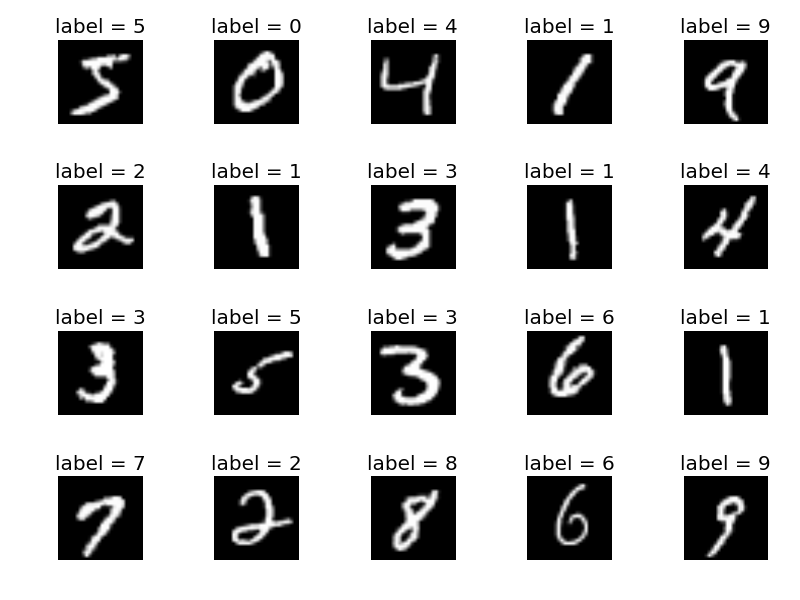
\includegraphics[width=\linewidth]{img/2_mnist.png}
        \caption{MNIST dataset}
    \end{subfigure}
    \hfill % optional; add some horizontal spacing
    \begin{subfigure}[b]{0.45\linewidth}
        \centering
        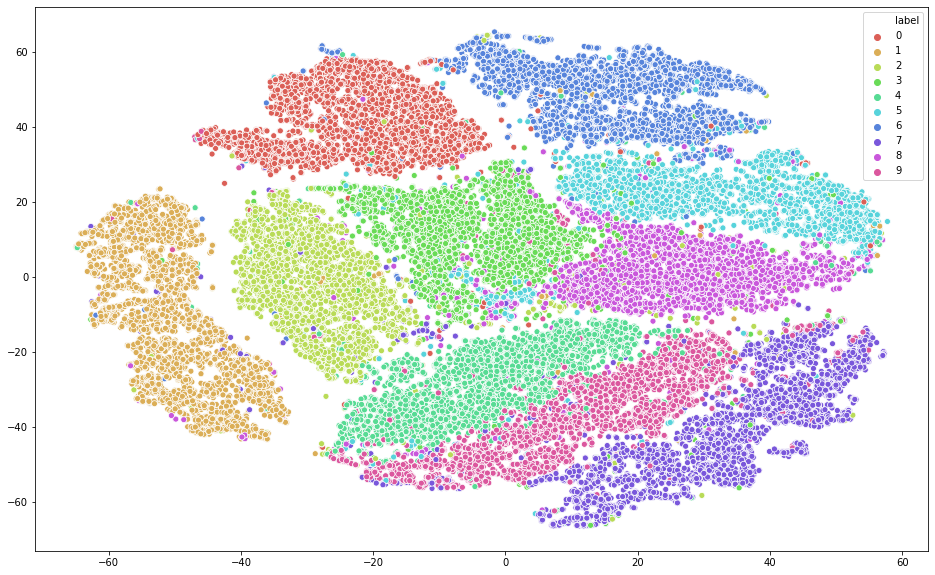
\includegraphics[width=\linewidth]{img/2_mnist-tsne.png}
        \caption{t-SNE visualisation on MNIST dataset}
        \label{fig:mnist-tsne}
    \end{subfigure}
    \caption{{\footnotesize MNIST dataset (dimension 10) and its corresponding t-SNE visualisation}}
    \label{fig:mnist-tsne}
\end{figure}




\end{enumerate}


\section{Supervised Learning}
Supervised learning assumes that we have access to input-output pairs of datapoints, $(\bm{x}, \bm{y})$, with $\bm{x} \in \mathbb{R}^n$ and $\bm{y} \in \mathbb{R}^m$, forming our dataset\sidenote{The slides replaced $K$ with $N$. Notation!} $\{(\bm{x}^{(i)}, \bm{y}^{(i)})\}_{i=1}^N$. 


\section{Linear Regression Model}
Assuming a domain of $\mathbb{R}^n$ and a one-dimensional co-domain, we can write our model as $f(\bm{x}) = \bm{x}^\top \bm{\theta}$. Thus we have:




\[
\hat{y}^{(i)} = \bm{x}^{(i)\top} \bm{\theta}
\]

The goal of learning is to find $\bm{\theta}$ such that $\hat{y}^{(i)} \approx y^{(i)}$. \marginnote{You may recall linear models written as affine transformations: $y = mx + b$, where $b$ is the bias or constant term – this makes the model affine and not linear. Linear models refers to the relationship between model parameters and predictions via a linear transformation.
}



\defb{Linear Transformation}{
A linear transformation between two vector spaces $V$ and $W$ is a map 

$$T : V \rightarrow W$$

such that:

\begin{itemize}
    \item $T(v_1 + v_2) = T(v_1) + T(v_2) \quad \forall v_1, v_2 \in V$
    \item $T(\alpha v) = \alpha T(v) \quad \forall v \in V \text{ and scalar }\alpha $
\end{itemize}

}

\marginnote[-70pt]{
    \defsb{Affine Transformations}{
        Affine transformations are more general than linear transformations, because they include not only scaling and rotation, but also translations.
    }
}


Now we are faced with something interesting: $T(\mb{0}) = \mb{0}$. According to our affine transformation $f(x) = mx+b $ where $m,b \in \mathbb{R}$, we have $f(0x) = b \neq 0f(x)$, which doesn't allow us to have a bias term $b$. This is easily fixed with a straightforward modification to capture the affine transformation $f(x) = mx + b$: we just add a feature to the input vector $x$ that is always equal to 1, then the corresponding weight for this feature becomes the bias. Introduce:

\begin{equation}
    \phi(x) : \mathbf{R} \Rightarrow \mathbf{R}^2 \quad \text{such that } \phi(x) = \begin{bmatrix} 1 \\ x \end{bmatrix} 
\end{equation}

\noindent We then need parameter vector $\theta = \begin{bmatrix} b \\ m \end{bmatrix}$. 

\noindent We then have the model 
\begin{equation}
    \hat{y} = \phi(x)^\top \theta \Rightarrow \begin{bmatrix} 1 & x \end{bmatrix}  \begin{bmatrix} b \\ m \end{bmatrix} = b + mx
\end{equation}

\section{Basis Expansion}
As seen in the previous section, a model that was once restricted to lines through the origin ahs been expanded to fit the affine transformation with the aid of Basis Expansion. We can also more generally utilise it to model non-linear relationships.

\bigskip

The key idea of basis expansion is to expand a one-dimensional feature into many dimensions, and use non-linear functions to increase the expressiveness of the model.

\subsection{Example Polynomial Basis Expansion}
A one dimensional domain $x \in \mathbb{R}$ and a one dimensional co-domain $y \in \mathbb{R}$ is assumed. Our model is $\hat{y} = \phi(x)^\top \theta$. \bigskip


We choose the basis:

\begin{equation}
    \phi(x) = \begin{bmatrix} 1 \\ x \\ x^2 \end{bmatrix} \quad \phi(x) : \R^1 \rightarrow \R^3
\end{equation}

and weights:

\begin{equation}
    \theta \in \mathbb{R}^3
\end{equation}

We finally have the fully expanded function\marginnote{We use the dot product instead of transposing, for clarity of notation.}:

\begin{equation}
    \hat{y} = \begin{bmatrix} 1 \\ x \\ x^2 \end{bmatrix} \cdot \begin{bmatrix} \theta_0 \\ \theta_1 \\ \theta_2 \end{bmatrix} = \theta_0 + \theta_1 x + \theta_2 x^2
\end{equation}

This example model is a quadratic polynomial. 

\subsection{Another Example Polynomial Basis Expansion}
Again, given our model is $\hat{y} = \phi(\mb{x})^\top \theta$ where $y \in \R $ and $\mb{x} \in \R^2$. We can use the basis

\begin{equation} 
    \phi(\mb{x}) \Rightarrow \phi\left(\begin{bmatrix} x_1 \\ x_2 \end{bmatrix}\right) = \begin{bmatrix} 1 \\ x_1 \\ x_2 \\ x_1x_2 \\ x_1^2 \\ x_2^2 \end{bmatrix} \quad \phi(x) : \mbb{R}^2 \rightarrow \mbb{R}^6
\end{equation}

and with a new set of corresponding weights, we have:

\begin{equation}
    \hat{y} = \begin{bmatrix} 1 \\ x_1 \\ x_2 \\ x_1x_2 \\ x_1^2 \\ x_2^2 \end{bmatrix} \cdot  \begin{bmatrix} \theta_0 \\ \theta_1 \\ \theta_2 \\ \theta_3 \\ \theta_4 \\ \theta_5 \end{bmatrix} = \theta_0 + \theta_1 x_1 + \theta_2 x_2 + \theta_3 x_1x_2 + \theta_4 x_1^2 + \theta_5 x_2^2 \quad \theta \in \mathbb{R}^6
\end{equation}

\section{Radial Basis Function Kernel}

Polynomial basis expansion is just a single flabour of basis expansion. Another widely-used form of basis is the kernel basis expansion. One popular example is the radial basis function kernel (RBF kernel), which is a generalisation of the polynomial basis expansion. \bigskip

It takes in a fixed parameter $\gamma > 0$, defined as 

\begin{equation}
    \kappa(x, x') = \exp(-\gamma ||x - x'||^2)
\end{equation}

where $||x - x'||^2$ is the squared Euclidean distance (or more appropriately, the $L_2$ Norm) between $x$ and $x'$. In practice, one picks fixed centres $x$ and the basis expansion computes the expanded feature set w.r.t the distance to these centres.\sidenote[][-130pt]{There is more nuance to this: you may have noticed that kernel functions take in two points, unlike the polynomial basis expansion $\phi$ taking in a single point. This is because for each of the $n$ points, we compute pairwise similarities with a point's other points, and then construct a feature vector for each point, where each point $x$ is transformed into a $n$-dimensional feature vector where each dimension represents the similarity between $x$ and one of the $n$ points.  \bigskip

For example, given a dataset with three points $x_1, x_2, x_3$, and a radial basis function $\kappa(x, x')$, the RBF kernel matrix might look like this:

\begin{equation*}
    K = \begin{bmatrix} \kappa(x_1, x_1) & \kappa(x_1, x_2) & \kappa(x_1, x_3) \\ \kappa(x_2, x_1) & \kappa(x_2, x_2) & \kappa(x_2, x_3) \\ \kappa(x_3, x_1) & \kappa(x_3, x_2) & \kappa(x_3, x_3) \end{bmatrix}
\end{equation*}

\noindent where the feature vector for $x_1$ as an example would be 
\[\begin{bmatrix} \kappa(x_1, x_1) & \kappa(x_1, x_2) & \kappa(x_1, x_3) \end{bmatrix}\]

\noindent This is related to the use of the \href{https://medium.com/@zxr.nju/what-is-the-kernel-trick-why-is-it-important-98a98db0961d}{kernel trick.}

}

\bigskip

\begin{itemize}
    \item It is easy to see that the kernel basis expansion $\kappa(x, x')$ has a minimum value of 0. It takes a maximum value of 1 when $x = x'$ . 
    \item When two points $x$ and $x'$ are far apart, the kernel value is closer to 0, and when they are closer together, the kernel value is closer to 1. 

    \item It is quite akin to a simiarity score, and that a smaller value of $\gamma$ leads to larger similarity scores (see Figure \ref{fig:rbf_kernel}).
    
    \item It is also symmetric, $\kappa(x, x') = \kappa(x', x)$, and is always positive. 
\end{itemize}

\bigskip
\begin{figure}[h]
    \centering
    \begin{tikzpicture}
    \begin{axis}[
        width=12cm,
        height=8cm,
        xlabel={$\|x - x'\|$},
        ylabel={$K(X_1, X_2)$},
        grid=major,
        domain=-10:10,
        samples=100,
        xtick={-10,-8,...,10},
        ytick={0,0.2,...,1},
        enlargelimits=false,
        legend pos=outer north east,
        axis lines=middle,
        xlabel style={at={(axis description cs:1.15,0.05)},anchor=north},
        ylabel style={at={(axis description cs:0.05,1)},anchor=south},
        title={RBF Kernel for $\kappa = 1/2$, graph of $\exp(-x^2/2)$},
        ymin=0, ymax=1,
        xmin=-10, xmax=10
    ]
        \addplot [
            blue,
            thick,
            domain=-10:10,
        ]
        {exp(-x^2/2)};
        
        % Highlight regions
        \draw [fill=blue, opacity=0.1] (axis cs:-10,0) rectangle (axis cs:-4,1);
        \draw [fill=blue, opacity=0.1] (axis cs:4,0) rectangle (axis cs:10,1);
        
        % Add region labels
        \node at (axis cs:-7,0.1) [anchor=north] {Dissimilar};
        \node at (axis cs:7,0.1) [anchor=north] {Dissimilar};
        \node at (axis cs:0,0.1) [anchor=north] {Similar};
    
    \end{axis}
    \end{tikzpicture}
    \caption{RBF Kernel for $\kappa = 1/2$, graph of $\exp(-x^2/2)$. Areas of dissimilarity are noted when the kernel values are negligible.}
    \label{fig:rbf_kernel}
    \end{figure}
    
    The RBF kernel is actually a special case of the polynomial basis expansion, where 


\subsection{Example Radial Basis Function Kernel}
Given a one-dimensional domain and a one-dimensional co-domain, we have the model $\hat{y} = \phi(x)^\top \theta$.

\begin{equation}
    \phi(x) = \exp(-\gamma ||x - x'||^2) \quad \phi(x) : \mathbb{R}^1 \rightarrow \mathbb{R}^1
\end{equation}

and with a new set of corresponding weights, we have:

\begin{equation}
    \hat{y} = \exp(-\gamma ||x - x'||^2) \cdot \begin{bmatrix} \theta_0 \\ \theta_1 \end{bmatrix} = \theta_0 \exp(-\gamma ||x - x'||^2) + \theta_1
\end{equation}


\section{Linear Algebra}









\chapter{Generalised Linear Models \& Gradient Descent}

\sn{Course Structure}{This part's additional materials will only be helpful after Chapter 6. Divorcing GLMs from their probabilistic context is rarely done, and is only done here for pedagogical purposes.}

Thus far we have utilised basis expansion to improve linear models. These models, especially with polynomial basis expansion, are great for modelling variables $y$ that vary constantly with respect to either their features or basis-expanded features.  Even though they are a arbitrarily powerful function approximator (formal statement will be discussed later in the course), they run the risk of overfitting (Chapter 5).  We motivate that data assumptions and model assumptions are different.

\defb{Gradient Notation}{
    In this course, vectors are assumed to be column vectors by default:

    \[
        \bm{b} \in \mathbb{R}^n = \bm{b} \in \mathbb{R}^{n \times 1}
    \]

    Gradients of vector-valued functions are, by convention, row vectors:

    \[
        f(\bm{b}) : \mathbb{R}^n \to \mathbb{R} \implies \nabla_{\bm{b}} f(\bm{b}) \in \mathbb{R}^{1 \times n}
    \]

    \[
        f(\bm{b}) : \mathbb{R}^n \to \mathbb{R}^m \implies \nabla_{\bm{b}} f(\bm{b}) \in \mathbb{R}^{m \times n}
    \]

    This layout is referred to as the "numerator" layout.
}

\section{Generalised Linear Models}
Generalised Linear Models use a single non-linear funciton to encode our beliefs about the output of our model, with the general form:

\begin{equation}
    \bm{y} = g^{-1}(\theta ^\top \bm{x})
\end{equation}

$g$ is the ``link'' function, traditionally associated with a probability density function from the exponential family.  However, we will later discuss when this interpretation will become very useful. A brief overview why GLMs are useful:
\begin{itemize}
    \item They are flexible with different data distributions. Standard linear regression assumes a normal distribution of errors or outputs, but GLMs can model other distributions such as Poisson, Bernoulli/Binomial, or Poisson.
    \item Linear regression assumes that the output $y$ is directly a linear function of the inputs (which we can transform from $x$ as part of the basis expansion). GLM assumes that some transformation of $y$ via the link function $g$ is linear in the inputs. It transforms the output variable instead of the input variables.
\end{itemize}


\subsection{Poisson Regression}
In many applications, we want to predict count information: e.g. how many people in a house, or the number of accidents in a city yearly. However linear regression models do not have restricted outputs and can predict negative values. Poisson Regression is a GLM that addresses this. \bigskip

Example: I want to predict the number of times a ship will get damaged in a particular period, given some information about the ship.

\begin{table}[h!]
    \centering
    \begin{tabular*}{\linewidth}{@{\extracolsep{\fill}} l l l r r}
        \toprule
        \textbf{TYPE} & \textbf{YEAR} & \textbf{PERIOD} & \textbf{MONTHS} & \textbf{Y} \\
        \midrule
        b & 1965-69 & 1975-79 & 20370 & 53 \\
        b & 1970-74 & 1960-74 & 7064  & 12 \\
        b & 1970-74 & 1975-79 & 13099 & 44 \\
        b & 1975-79 & 1960-74 & 0     & 0  \\
        b & 1975-79 & 1975-79 & 7117  & 18 \\
        b & 1960-64 & 1960-74 & 44882 & 39 \\
        b & 1960-64 & 1975-79 & 17176 & 29 \\
        b & 1965-69 & 1960-74 & 28609 & 58 \\
        c & 1960-64 & 1960-74 & 1179  & 1  \\
        c & 1960-64 & 1975-79 & 552   & 1  \\
        \bottomrule
    \end{tabular*}
    \caption{Types of damages and the number of times they occurred in a particular period.}
    \label{tab:example_table}
\end{table}

Consider a design matrix $\bm{X}' \in \mathbb{R}^{n \times m}$ and response variables are collected into response vector $\bm{y} \in \mathbb{R}^n$. \bigskip

We augment the design matrix, adding a 1 to the end of each vector (affine basis expansion).

\begin{equation}
    \bm{X}' \rightarrow \bm{X} \in \mathbb{R}^{(n+1) \times m}
\end{equation}

To achieve the desired strictly positive co-domain, we simply exponentiate:

\begin{equation}
    \hat{\bm{y}} = \exp(\bm{X} {\theta})
\end{equation}

The loss function is given by:

\begin{equation}
    \mathcal{L}(\theta) = \sum_{i=1}^{m} \left( y^{(i)} \bm{x}^{(i)^\top} \theta - \exp(\bm{x}^{(i)^\top} \theta) \right) - \sum_{i=1}^{m} \log\left(y^{(i)}!\right)
\end{equation}

The full context and derivation of this loss function will be covered in later chapters (early hint: it is the log-likelihood). This loss function does not have a closed-form solution. \bigskip

Instead, we can try to use MSE loss instead to find its gradient:

\begin{align*}
    \mathcal{L}(\theta) & = \frac{1}{m} (\hat{y} - y)^2                            \\
                        & = \frac{1}{m} (\exp(\bm{X}\theta) - y)^2                 \\
                        & \propto (\exp(\bm{X}\theta) - y)^2                       \\
                        & = (\exp(\bm{X}\theta) - y)^\top (\exp(\bm{X}\theta) - y)
\end{align*}

To compute the gradient, the loss is expressed as a summation:

\[
    \mathcal{L}(\theta) = \sum_{i=1}^{k} (\exp(\bm{X}_{i,:}^\top \theta) - y_i)^2
\]

where \(\bm{X}_{i,:}^\top\) is the \(i\)-th row of \(\bm{X}\). Applying the chain rule:

\[
    \frac{\partial}{\partial \theta} \left( \exp(\bm{X}_{i,:}^\top \theta) - y_i \right)^2 = 2 (\exp(\bm{X}_{i,:}^\top \theta) - y_i) \cdot \frac{\partial}{\partial \theta} \exp(\bm{X}_{i,:}^\top \theta)
\]

The derivative of \(\exp(\bm{X}_{i,:}^\top \theta)\) with respect to \(\theta\) is:

\[
    \frac{\partial}{\partial \theta} \exp(\bm{X}_{i,:}^\top \theta) = \exp(\bm{X}_{i,:}^\top \theta) \cdot \bm{X}_{i,:}^\top
\]

Thus, the gradient of each term is:

\[
    \frac{\partial}{\partial \theta} \left( \exp(\bm{X}_{i,:}^\top \theta) - y_i \right)^2 = 2 (\exp(\bm{X}_{i,:}^\top \theta) - y_i) \cdot \exp(\bm{X}_{i,:}^\top \theta) \cdot \bm{X}_{i,:}^\top
\]

Summing over all data points:

\[
    \nabla_\theta \mathcal{L}(\theta) = 2 \sum_{i=1}^{k} (\exp(\bm{X}_{i,:}^\top \theta) - y_i) \cdot \exp(\bm{X}_{i,:}^\top \theta) \cdot \bm{X}_{i,:}^\top
\]

In matrix form:

\[
    \nabla_\theta \mathcal{L}(\theta) = 2 \left( (\exp(\bm{X}\theta) - \bm{y}) \odot \exp(\bm{X}\theta) \right)^\top \bm{X}
\]

Here, \(\odot\) denotes element-wise multiplication.

\subsection{Logistic Regression}
In many applications, we would like to predict the class of a particular input e.g. classifying if an email is spam or not. The simplest case is binary classification, where the output is either 0 or 1. We take $\bm{y} \in [0,1]$ in this case.

\begin{figure}[h!]
    \centering
    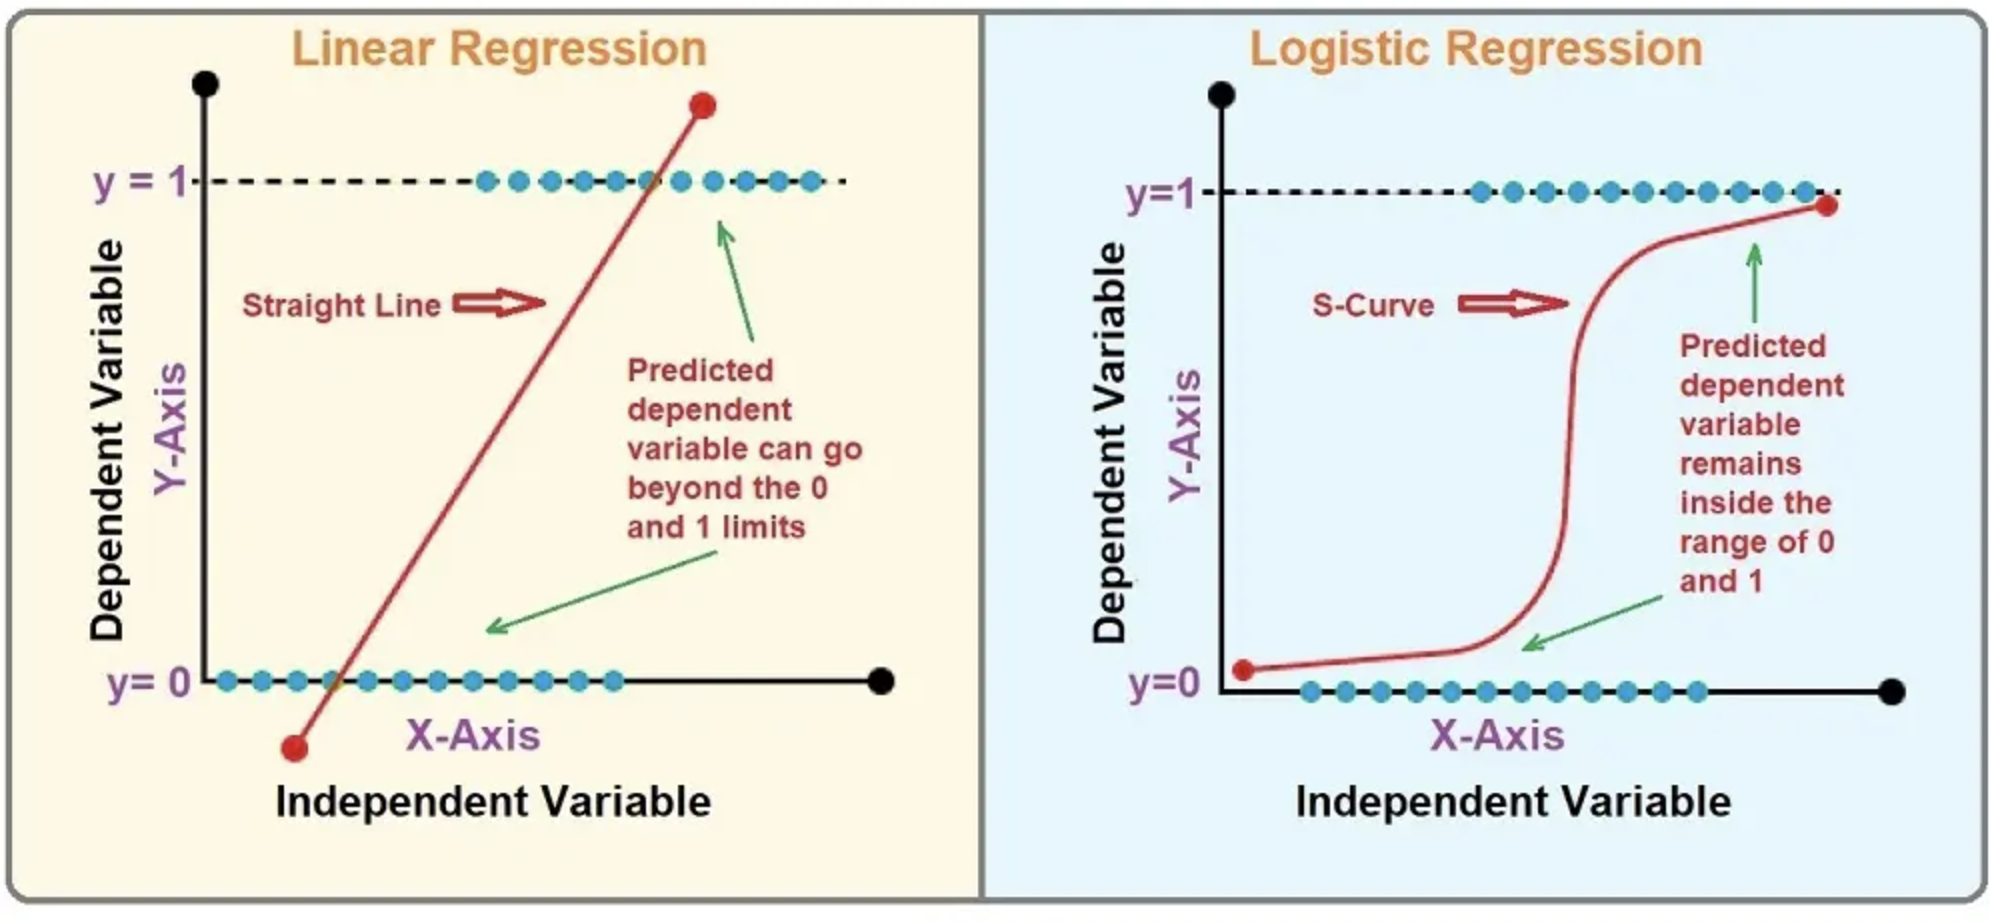
\includegraphics[width=1\textwidth]{img/3_lr_vs_logistic.png}
    \caption{Using a contrived, unbalanced dataset, we visualise an intuitive case where the non-linearity in  logistic regression helps us model the data more accurately compared to linear regression.}
\end{figure}


Consider a design matrix $\bm{X}' \in \mathbb{R}^{n \times m}$ and response variables are collected into response vector $\bm{y} \in \mathbb{R}^n$ where entries $y_i \in \{0,1\}$. \bigskip

We augment the design matrix as usual, adding a 1 to the end of each vector (affine basis expansion).

\begin{equation}
    \bm{X}' \rightarrow \bm{X} \in \mathbb{R}^{(n+1) \times m}
\end{equation}

We then apply the logistic function so that the range of the output is $[0,1]$:
\begin{equation}
    \sigma(x) = \frac{1}{1 + \exp(-x)}
\end{equation}

The loss function we desire is the negative log-likelihood for the Bernoulli distribution which is:

\[
    \mathcal{L}(\theta) = -\frac{1}{m} \sum_{i=1}^{m} \left( y^{(i)} \log(\sigma(\theta^\top \bm{x}^{(i)})) + (1 - y^{(i)}) \log(1 - \sigma(\theta^\top \bm{x}^{(i)})) \right)
\]

where \(\sigma(x) = \frac{1}{1 + \exp(-x)}\) is the logistic function. \bigskip

Since the minimiser of this equation cannot be solved in closed form, we use numerical methods such as gradient descent.

The gradient of the loss function with respect to \(\theta\) is:

\[
    \nabla_\theta \mathcal{L}(\theta) = -\frac{1}{m} \sum_{i=1}^{m} \left( y^{(i)} (1 - \sigma(\theta^\top \bm{x}^{(i)})) - (1 - y^{(i)}) \sigma(\theta^\top \bm{x}^{(i)}) \right) \bm{x}^{(i)}
\]

This simplifies to:

\[
    \nabla_\theta \mathcal{L}(\theta) = -\frac{1}{m} \sum_{i=m}^{k} \left( y^{(i)} - \sigma(\theta^\top \bm{x}^{(i)}) \right) \bm{x}^{(i)}
\]


\refb{Linear Models for Classification}{
\textbf{Linear models for classification, Chapter 4.1 - 4.1.3 (page 179) Bishop (2006).}
\bigskip

Note that we did not use the MSE approach here– for a more detailed discussion on why this is not ideal, refer to the above reference. \smallskip


\begin{center}
    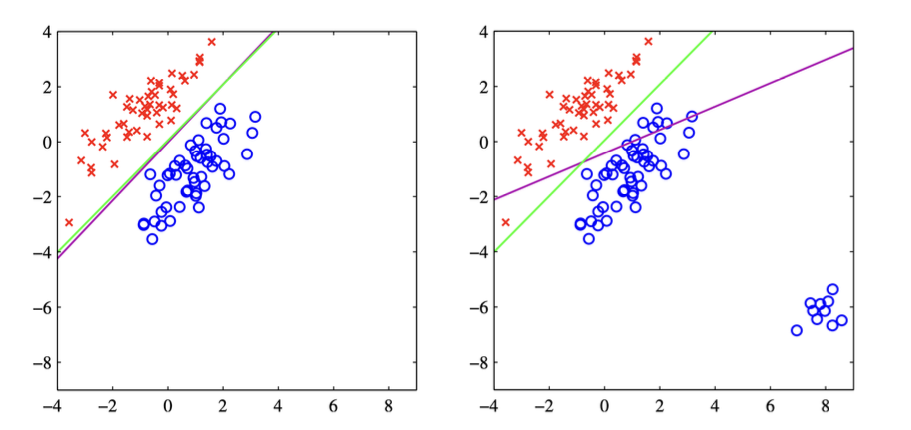
\includegraphics[width=1\textwidth]{img/3_logistic_outliers.png}
\end{center}
{\small Figure and caption text from Bishop 2006: The left plot shows data from two classes, denoted by red crosses and blue circles, together with the decision boundary found by least squares (magenta curve) and also by the logistic regression model (green curve). The right-hand plot shows the corresponding results obtained when extra data points are added at the bottom left of the diagram, showing that least squares is highly sensitive to outliers, unlike logistic regression.}

\bigskip





Why we do not use the MSE loss:
\begin{itemize}
    \item The MSE itself is meant for continuous output values, so it does not make sense to use it for binary classification.
    \item The squaring of error in MSE amplifies the impact of large errors or outliers, thus a few outliers can disproportionately influence the whole model.
\end{itemize}


}

\section{Gradient Descent}

Gradient descent is the core algorithm behind the \textit{learning} portion of many ML algorithms, by fining the minimum of a (loss) function The idea is to iteratively take steps in the direction of the steepest descent, which is determined by the gradient of the function. The gradient is denoted by \(\nabla\), with a subscript indicating the variable we are differentiating with respect to.

The basic form of gradient descent is:

\[
    \theta^{(t+1)} = \theta^{(t)} + \alpha \nabla_\theta \mathcal{L}(f^\theta, \bm{X}, \bm{y}),
\]

where \(\alpha\) is the learning rate, and \(\theta^{(0)} \sim \mathcal{N}(0, 1)\).\bigskip


We interpret (in the two-dimensional weight case) \(\mathcal{L}(f^\theta, \bm{X}, \bm{y})\) as a height we want to minimise, and visualise \(\theta\) as a puck being pushed in the direction that lowers the height.\bigskip

Some factors that affect the convergence of gradient descent are:
\begin{itemize}
    \item Learning rate: If the learning rate is too high, the puck may overshoot the minimum. If it is too low, the puck may take too long to reach the minimum.
    \item Iterations: A sufficient number of iterations is needed to reach the minimum – if not enough, the optimal loss is not achieved.
\end{itemize}


\begin{figure}[h!]
    \centering
    % First subfigure
    \begin{subfigure}[b]{0.49\linewidth}
        \centering
        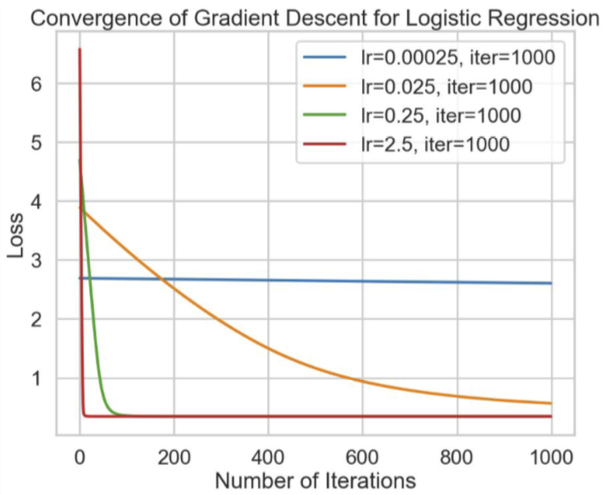
\includegraphics[width=\linewidth]{img/3_logr_gd.png}
        \caption{Convergence of the loss during gradient descent for logistic regression.}
        \label{fig:logr_gd}
    \end{subfigure}
    % Second subfigure
    \begin{subfigure}[b]{0.49\linewidth}
        \centering
        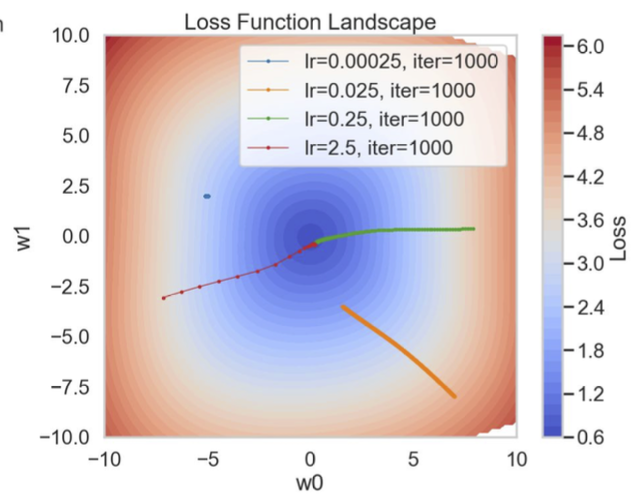
\includegraphics[width=\linewidth]{img/3_logr_loss_function_landscape.png}
        \caption{Loss function landscape and path of the parameter as it moves.}
        \label{fig:logr_loss_landscape}
    \end{subfigure}

    \caption{Effect of learning rate on logistic regression training. (a) The convergence of the loss over iterations, interpreted as the height of the puck in the bowl. (b) A visualisation of the parameter's path in the loss function landscape.}
    \label{fig:logr_learning_rate_effect}
\end{figure}

\begin{figure}[h!]
    \centering
    % First subfigure
    \begin{subfigure}[b]{0.49\linewidth}
        \centering
        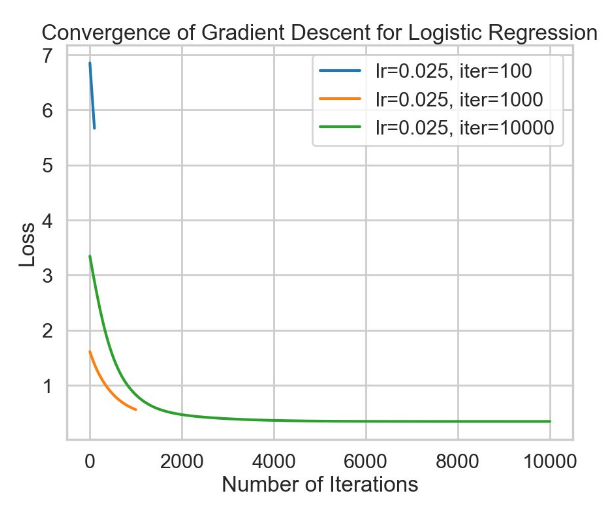
\includegraphics[width=\linewidth]{img/3_logr_gd_iters.png}
        \caption{Convergence of the loss during gradient descent for logistic regression with different numbers of iterations.}
        \label{fig:logr_gd_iters}
    \end{subfigure}
    % Second subfigure
    \begin{subfigure}[b]{0.49\linewidth}
        \centering
        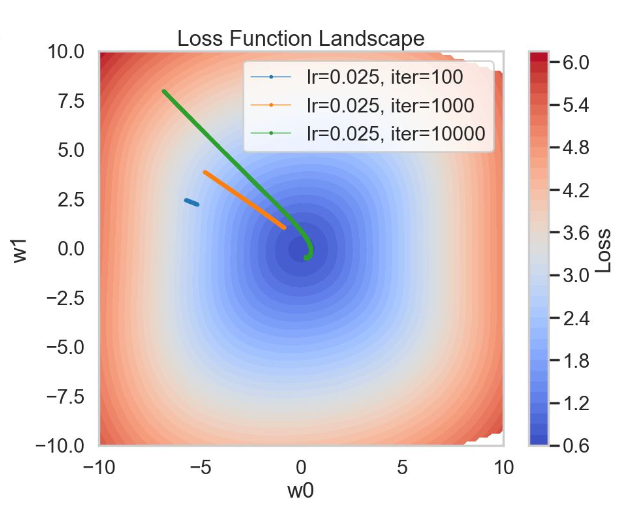
\includegraphics[width=\linewidth]{img/3_logr_loss_function_landscape_iters.png}
        \caption{Loss function landscape and parameter's path with different iterations.}
        \label{fig:logr_loss_landscape_iters}
    \end{subfigure}

    \caption{Effect of number of iterations on the learning of our logistic regression model. (a) The convergence of the loss over iterations, interpreted as the height of the puck in the bowl. (b) A visualization of the parameter's path in the loss function landscape for different iterations.}
    \label{fig:logr_iterations_effect}
\end{figure}

\newpage
\subsection{Complexity of OLS Closed-Form Solution}
It is awkward to compare Ordinary Least Squares (OLS) to Gradient Descent (GD) in Generalised Linear Models (GLM), as we cannot directly use the OLS in GLMs. \footnote{OLS assumes the errors in the model are normally distributed and have constant variance (called homoscedasticity), a common regression assumption. But Generalised Linear Models don't have this condition, and errors can be distributed via the Poisson, binomial, or exponential families. GLMs use Maximum Likelihood Estimation (MLE) instead of the OLS, which will be explained in later chapters. } \bigskip

We can, however, consider the complexity of Ordinary Least Squares (OLS) with Gradient Descent (GD) for Generalised Linear Models (GLMs). \bigskip


First, consider the OLS closed-form solution:
\[
    \theta = (\bm{X}^\top \bm{X})^{-1} \bm{X}^\top \bm{y}
\]

\begin{enumerate}
    \item The matrix product $\bm{X}^\top \bm{X}$ involves multiplying two matrices \( A \in \mathbb{R}^{n \times m} \) and \( B \in \mathbb{R}^{m \times n} \), which has the general form:
          \[
              \bm{C}_{i,j} = \sum_{k=1}^{l} \bm{A}_{i,k} \bm{B}_{k,j}
          \]
          \begin{itemize}
              \item Since $k$ is our dummy index, it gets summed over $l$ times.
              \item It is repeated for each element in the resulting matrix $\bm{C}$.
              \item Remember, the data matrix $\bm{X}$ is of size \( n \times m \), so that's \( n \) features and \( m \) samples.
          \end{itemize}
          This operation has a complexity of \( O(n l m) \).

          \begin{figure}
              \centering
              \begin{tikzpicture}[scale=0.5]

                  % Matrix A
                  \matrix[matrix of math nodes,left delimiter={[},right delimiter={]}, nodes={font=\small}, inner sep=0.5pt, row sep = 15pt, column sep = 0pt] (A) {
                          A_{1,1} & A_{1,2} & \dots & A_{1,m} \\
                          A_{2,1} & A_{2,2} & \dots & A_{2,m} \\
                          \vdots  & \vdots  & \ddots & \vdots \\
                          A_{n,1} & A_{n,2} & \dots & A_{n,m} \\
                      };

                  % Matrix B
                  \matrix[matrix of math nodes,left delimiter={[},right delimiter={]}, nodes={font=\small}, inner sep=0.5pt, column sep = 5pt] (B) [right=1.5cm of A] {
                          B_{1,1} & B_{1,2} & \dots & B_{1,n} \\
                          B_{2,1} & B_{2,2} & \dots & B_{2,n} \\
                          \vdots  & \vdots  & \ddots & \vdots \\
                          B_{m,1} & B_{m,2} & \dots & B_{m,n} \\
                      };

                  % Matrix C
                  \matrix[matrix of math nodes,left delimiter={[},right delimiter={]}, nodes={font=\small}, inner sep=0.5pt, row sep =15pt, column sep = 0pt] (C) [right=1.5cm of B] {
                          C_{1,1} & C_{1,2} & \dots & C_{1,n} \\
                          C_{2,1} & C_{2,2} & \dots & C_{2,n} \\
                          \vdots  & \vdots  & \ddots & \vdots \\
                          C_{n,1} & C_{n,2} & \dots & C_{n,n} \\
                      };

                  % Place the multiplication and equals signs with better spacing
                  \node at ($(A.east)+(1.7,0)$) {\large $\times$};
                  \node at ($(B.east)+(1.7,0)$) {\large $=$};

                  % Highlight the first row of A with light transparent red fill
                  \draw[thick, red, fill=red!30, fill opacity=0.3, rounded corners]
                  ($(A-1-1.north west)+(-0.1,0.1)$) -- ($(A-1-4.north east)+(0.1,0.1)$) --
                  ($(A-1-4.south east)+(0.1,-0.1)$) -- ($(A-1-1.south west)+(-0.1,-0.1)$) -- cycle;

                  % Highlight the first column of B with light transparent blue fill
                  \draw[thick, blue, fill=blue!30, fill opacity=0.3, rounded corners]
                  ($(B-1-1.north west)+(-0.1,0.1)$) -- ($(B-4-1.south west)+(-0.1,-0.1)$) --
                  ($(B-4-1.south east)+(0.1,-0.1)$) -- ($(B-1-1.north east)+(0.1,0.1)$) -- cycle;

                  % Highlight the top-left element of C with light transparent green fill
                  \draw[thick, green, fill=green!30, fill opacity=0.3, rounded corners]
                  ($(C-1-1.north west)+(-0.1,0.1)$) -- ($(C-1-1.north east)+(0.1,0.1)$) --
                  ($(C-1-1.south east)+(0.1,-0.1)$) -- ($(C-1-1.south west)+(-0.1,-0.1)$) -- cycle;

              \end{tikzpicture}
              \caption{Matrix product \(\bm{X}^\top \bm{X}\) involves multiplying two matrices \(A \in \mathbb{R}^{n \times m}\) and \(B \in \mathbb{R}^{m \times n}\), resulting in a matrix \(C \in \mathbb{R}^{n \times n}\) with a complexity of \(O(n^2 m)\).}
          \end{figure}

          % \footnote{$\bm{X}^\top\bm{X}$ is really just a square matrix, we only keep $n$ and $m$ separate to understand which side of the index is being used.}

          Since \( \bm{X}^\top \bm{X} \) is of size \( n \times n \)  , the total complexity of computing this matrix product is \( O(n^2 m) \).

          \[
              \theta = \underbrace{(\bm{X}^\top \bm{X})^{-1}}_{n \times n}
              \underbrace{\bm{X}^\top}_{n \times m}
              \underbrace{\bm{y}}_{m \times 1}
          \]

    \item Next, matrix inversion for \( (\bm{X}^\top \bm{X})^{-1} \) (which is square) has complexity\footnote{There are several algorithms for matrix inversion that are better than cubic, but we stick to $O(n^3)$.}  \( O(n^3) \). Combining these operations, the current total complexity becomes:
          \[
              O(n^2 m + n^3)
          \]
    \item We multiply the \( \bm{X}^\top \bm{y} \) term. This is a matrix vector product between $\bm{A} \in \mathbb{R}^{n \times m}$ and $\bm{b} \in \mathbb{R}^{m \times 1}$ with complexity $O(mn)$ (see Figure \ref{fig:matrix_vector_product_1}).
          \[
              \bm{c}_j = \sum^n_{i=1} \bm{A}_{i,j} \bm{b}_i
          \]
          \begin{figure}[h!]
              \centering
              \begin{tikzpicture}[scale=0.5]

                  % Matrix X^T
                  \matrix[matrix of math nodes,left delimiter={[},right delimiter={]}, nodes={font=\small}, inner sep=0.5pt, column sep = 5pt] (X) {
                          X_{1,1} & X_{1,2} & \dots & X_{1,n} \\
                          X_{2,1} & X_{2,2} & \dots & X_{2,n} \\
                          \vdots  & \vdots  & \ddots & \vdots \\
                          X_{m,1} & X_{m,2} & \dots & X_{m,n} \\
                      };

                  % Vector y
                  \matrix[matrix of math nodes,left delimiter={[},right delimiter={]}, nodes={font=\small}, inner sep=0.5pt, row sep = 15pt, column sep = 0pt] (y) [right=1.5cm of X] {
                          y_{1} \\
                          y_{2} \\
                          \vdots  \\
                          y_{n} \\
                      };

                  % Result vector c
                  \matrix[matrix of math nodes,left delimiter={[},right delimiter={]}, nodes={font=\small}, inner sep=0.5pt] (c) [right=1.5cm of y] {
                          c_1 \\
                          c_2 \\
                          \vdots  \\
                          c_m \\
                      };

                  % Place the multiplication and equals signs with better spacing
                  \node at ($(X.east)!0.5!(y.west)$) {\large $\times$};
                  \node at ($(y.east)!0.5!(c.west)$) {\large $=$};

                  % Highlight the first row of X^T with light transparent red fill
                  \draw[thick, red, fill=red!30, fill opacity=0.3, rounded corners]
                  ($(X-1-1.north west)+(-0.1,0.1)$) -- ($(X-1-4.north east)+(0.1,0.1)$) --
                  ($(X-1-4.south east)+(0.1,-0.1)$) -- ($(X-1-1.south west)+(-0.1,-0.1)$) -- cycle;

                  % Highlight the first column of y with light transparent blue fill
                  \draw[thick, blue, fill=blue!30, fill opacity=0.3, rounded corners]
                  ($(y-1-1.north west)+(-0.1,0.1)$) -- ($(y-4-1.south west)+(-0.1,-0.1)$) --
                  ($(y-4-1.south east)+(0.1,-0.1)$) -- ($(y-1-1.north east)+(0.1,0.1)$) -- cycle;

                  % Highlight the top-left element of c with light transparent green fill
                  \draw[thick, green, fill=green!30, fill opacity=0.3, rounded corners]
                  ($(c-1-1.north west)+(-0.1,0.1)$) -- ($(c-1-1.north east)+(0.1,0.1)$) --
                  ($(c-1-1.south east)+(0.1,-0.1)$) -- ($(c-1-1.south west)+(-0.1,-0.1)$) -- cycle;

              \end{tikzpicture}
              \caption{Matrix-vector product for $\bm{X}^\top \bm{y}$}
              \label{fig:matrix_vector_product_1}
          \end{figure}

    \item We then multiply $(\bm{X}^\top \bm{X})^{-1}$ with \( \bm{X}^\top \bm{y} \). This is a matrix vector product between $\bm{A} \in \mathbb{R}^{n \times n}$ and $\bm{b} \in \mathbb{R}^{n \times 1}$ with complexity $O(n^2)$ (see Figure \ref{fig:matrix_vector_product_2}).
          \[
              \bm{c}_j = \sum^n_{i=1} \bm{A}_{i,j} \bm{b}_i
          \]
          \begin{figure}[h!]
              \centering
              \begin{tikzpicture}[scale=0.5]

                  % Matrix X^T
                  \matrix[matrix of math nodes,left delimiter={[},right delimiter={]}, nodes={font=\small}, inner sep=0.5pt, column sep = 5pt] (X) {
                          X_{1,1} & X_{1,2} & \dots & X_{1,n} \\
                          X_{2,1} & X_{2,2} & \dots & X_{2,n} \\
                          \vdots  & \vdots  & \ddots & \vdots \\
                          X_{n,1} & X_{n,2} & \dots & X_{n,n} \\
                      };

                  % Vector y
                  \matrix[matrix of math nodes,left delimiter={[},right delimiter={]}, nodes={font=\small}, inner sep=1pt, row sep = 15pt, column sep = 0pt] (y) [right=1.5cm of X] {
                          y_{1} \\
                          y_{2} \\
                          \vdots  \\
                          y_{n} \\
                      };

                  % Result vector c
                  \matrix[matrix of math nodes,left delimiter={[},right delimiter={]}, nodes={font=\small}, inner sep=1pt] (c) [right=1.5cm of y] {
                          c_1 \\
                          c_2 \\
                          \vdots  \\
                          c_n \\
                      };

                  % Place the multiplication and equals signs with better spacing
                  \node at ($(X.east)!0.5!(y.west)$) {\large $\times$};
                  \node at ($(y.east)!0.5!(c.west)$) {\large $=$};

                  % Highlight the first row of X^T with light transparent red fill
                  \draw[thick, red, fill=red!30, fill opacity=0.3, rounded corners]
                  ($(X-1-1.north west)+(-0.1,0.1)$) -- ($(X-1-4.north east)+(0.1,0.1)$) --
                  ($(X-1-4.south east)+(0.1,-0.1)$) -- ($(X-1-1.south west)+(-0.1,-0.1)$) -- cycle;

                  % Highlight the first column of y with light transparent blue fill
                  \draw[thick, blue, fill=blue!30, fill opacity=0.3, rounded corners]
                  ($(y-1-1.north west)+(-0.1,0.1)$) -- ($(y-4-1.south west)+(-0.1,-0.1)$) --
                  ($(y-4-1.south east)+(0.1,-0.1)$) -- ($(y-1-1.north east)+(0.1,0.1)$) -- cycle;

                  % Highlight the top-left element of c with light transparent green fill
                  \draw[thick, green, fill=green!30, fill opacity=0.3, rounded corners]
                  ($(c-1-1.north west)+(-0.1,0.1)$) -- ($(c-1-1.north east)+(0.1,0.1)$) --
                  ($(c-1-1.south east)+(0.1,-0.1)$) -- ($(c-1-1.south west)+(-0.1,-0.1)$) -- cycle;

              \end{tikzpicture}
              \caption{Matrix-vector product for $(\bm{X}^\top \bm{X})^{-1} \bm{X}^\top \bm{y}$}
              \label{fig:matrix_vector_product_2}
          \end{figure}



          We have
          \begin{equation}
              \theta =
              \underbrace{
                  \underbrace{
                      \left( \underbrace{\bm{X}^\top \bm{X}}_{O(n^2m)} \right)^{-1}
                  }_{O(n^3)}
                  \underbrace{
                      \bm{X}^\top \bm{y}
                  }_{O(nm)}}_{O(n^2)}
          \end{equation}

          and our final complexity is \( O(n^2 m + n^3) \).\marginnote{This is because we had $O(nm + n^2m + n^2 + n^3) = O(n(m + nm + n) + n^3) \Rightarrow  O(n^2 m + n^3)$} This can be quite inefficient for large datasets where $m$ is large! We alleviate this by using stochastic gradient descent.

          \subsection{Complexity of Stochastic Gradient Descent}

          Instead of having to compute the full OLS solution by inverting the matrix, we can iterate towards an approximate solution by taking the gradient of the loss function and applying it to gradient descent. \bigskip

          We then can optimize the computation by sub-sampling a \textit{batch} of the data, leading to \textit{stochastic gradient descent (SGD)}. The gradient for linear regression is given by:
          \[
              \bm{X}^\top (\bm{X} \theta - \bm{y})
          \]

          The operations comprise:
          \begin{itemize}
              \item Matrix-vector multiplication \( \bm{X} \theta \) has a complexity of \( O(b n) \) if \( \bm{X} \in \mathbb{R}^{b \times n} \), where \( b \) is the batch size, $\theta \in \mathbb{R}^{n \times 1}$, $n$ is the number of features.

                    \[
                        \bm{c}_j = \sum_{i=1}^{n} \bm{X}_{i,j} \theta_i
                    \]

                    \begin{figure}

                        \centering
                        \begin{tikzpicture}[scale=0.5]

                            % Matrix X^T
                            \matrix[matrix of math nodes,left delimiter={[},right delimiter={]}, nodes={font=\small}, inner sep=1pt] (X) {
                                    X_{1,1} & X_{1,2} & \dots & X_{1,n}  \\
                                    X_{2,1} & X_{2,2} & \dots & X_{2,n}  \\
                                    \vdots  & \vdots  & \ddots & \vdots  \\
                                    X_{b,1} & X_{b,2} & \dots & X_{b,n}  \\
                                };

                            % Vector theta
                            \matrix[matrix of math nodes,left delimiter={[},right delimiter={]}, nodes={font=\small}, inner sep=1pt] (theta) [right=1.5cm of X] {
                                    \theta_{1} \\
                                    \theta_{2} \\
                                    \vdots  \\
                                    \theta_{n} \\
                                };

                            % Result vector c
                            \matrix[matrix of math nodes,left delimiter={[},right delimiter={]}, nodes={font=\small}, inner sep=1pt] (c) [right=1.5cm of theta] {
                                    c_1 \\
                                    c_2 \\
                                    \vdots  \\
                                    c_b \\
                                };

                            % Place the multiplication and equals signs with better spacing
                            \node at ($(X.east)!0.5!(theta.west)$) {\large $\times$};
                            \node at ($(theta.east)!0.5!(c.west)$) {\large $=$};

                            % Highlight the first row of X^T with light transparent red fill
                            \draw[thick, red, fill=red!30, fill opacity=0.3, rounded corners]
                            ($(X-1-1.north west)+(-0.1,0.1)$) -- ($(X-1-4.north east)+(0.1,0.1)$) --
                            ($(X-1-4.south east)+(0.1,-0.1)$) -- ($(X-1-1.south west)+(-0.1,-0.1)$) -- cycle;

                            % Highlight the first column of theta with light transparent blue fill
                            \draw[thick, blue, fill=blue!30, fill opacity=0.3, rounded corners]
                            ($(theta-1-1.north west)+(-0.1,0.1)$) -- ($(theta-4-1.south west)+(-0.1,-0.1)$) --
                            ($(theta-4-1.south east)+(0.1,-0.1)$) -- ($(theta-1-1.north east)+(0.1,0.1)$) -- cycle;

                            % Highlight the top-left element of c with light transparent green fill
                            \draw[thick, green, fill=green!30, fill opacity=0.3, rounded corners]
                            ($(c-1-1.north west)+(-0.1,0.1)$) -- ($(c-1-1.north east)+(0.1,0.1)$) --
                            ($(c-1-1.south east)+(0.1,-0.1)$) -- ($(c-1-1.south west)+(-0.1,-0.1)$) -- cycle;

                        \end{tikzpicture}
                    \end{figure}
              \item $(\bm{X} \theta - \bm{y}) \in \mathbb{R}^{b \times 1}$ is a vector subtraction, which has a complexity of \( O(b) \).
              \item Gradient computation \( \bm{X}^\top (\bm{X} \theta - \bm{y}) \) also has a complexity of \( O(b n) \). $\bm{X}^\top \in \mathbb{R}^{n \times b}$, $(\bm{X} \theta - \bm{y}) \in \mathbb{R}^{b \times 1}$.
                    \[
                        \bm{c}_j = \sum_{i=1}^{b} \bm{X}_{i,j} \theta_i
                    \]

                    \begin{figure}

                        \centering
                        \begin{tikzpicture}[scale=0.5]

                            % Matrix X^T
                            \matrix[matrix of math nodes,left delimiter={[},right delimiter={]}, nodes={font=\small}, inner sep=0.5pt, row sep=15pt, column sep = 0pt] (X) {
                                    X_{1,1} & X_{1,2} & \dots & X_{1,b}  \\
                                    X_{2,1} & X_{2,2} & \dots & X_{2,b}  \\
                                    \vdots  & \vdots  & \ddots & \vdots  \\
                                    X_{n,1} & X_{n,2} & \dots & X_{n,b}  \\
                                };

                            % Vector theta
                            \matrix[matrix of math nodes,left delimiter={[},right delimiter={]}, nodes={font=\small}, inner sep=1pt] (theta) [right=1.5cm of X] {
                                    \theta_{1} \\
                                    \theta_{2} \\
                                    \vdots  \\
                                    \theta_{b} \\
                                };

                            % Result vector c
                            \matrix[matrix of math nodes,left delimiter={[},right delimiter={]}, nodes={font=\small}, inner sep=1pt] (c) [right=1.5cm of theta] {
                                    c_1 \\
                                    c_2 \\
                                    \vdots  \\
                                    c_n \\
                                };

                            % Place the multiplication and equals signs with better spacing
                            \node at ($(X.east)!0.5!(theta.west)$) {\large $\times$};
                            \node at ($(theta.east)!0.5!(c.west)$) {\large $=$};

                            % Highlight the first row of X^T with light transparent red fill
                            \draw[thick, red, fill=red!30, fill opacity=0.3, rounded corners]
                            ($(X-1-1.north west)+(-0.1,0.1)$) -- ($(X-1-4.north east)+(0.1,0.1)$) --
                            ($(X-1-4.south east)+(0.1,-0.1)$) -- ($(X-1-1.south west)+(-0.1,-0.1)$) -- cycle;

                            % Highlight the first column of theta with light transparent blue fill
                            \draw[thick, blue, fill=blue!30, fill opacity=0.3, rounded corners]
                            ($(theta-1-1.north west)+(-0.1,0.1)$) -- ($(theta-4-1.south west)+(-0.1,-0.1)$) --
                            ($(theta-4-1.south east)+(0.1,-0.1)$) -- ($(theta-1-1.north east)+(0.1,0.1)$) -- cycle;

                            % Highlight the top-left element of c with light transparent green fill
                            \draw[thick, green, fill=green!30, fill opacity=0.3, rounded corners]
                            ($(c-1-1.north west)+(-0.1,0.1)$) -- ($(c-1-1.north east)+(0.1,0.1)$) --
                            ($(c-1-1.south east)+(0.1,-0.1)$) -- ($(c-1-1.south west)+(-0.1,-0.1)$) -- cycle;

                        \end{tikzpicture}
                    \end{figure}



              \item We have
                    \[
                        \underbrace{\bm{X}^\top \underbrace{(\overbrace{\bm{X}\bm{\theta}}^{O(bn)} - \bm{y})}_{O(b)} }_{O(bn)}
                    \]
          \end{itemize}

          Performing \textit{stochastic gradient descent} in batches of size $b$, iterating \( k \) times results in a total complexity of:
          \[
              O(kbn)
          \]

          For the whole dataset where we just set the batch size to the size of the entire dataset $n$, the complexity is:
          \[
              O(kmn)
          \]

\end{enumerate}

\subsection{Complexity Comparison: OLS vs Gradient Descent}

Comparing the complexities:
\begin{itemize}
    \item OLS: \( O(n^2 m + n^3) \)
    \item Gradient Descent: \( O(kmn) \), with SGD reducing this to \( O(kbn) \)
\end{itemize}

If \( k < n \), gradient descent becomes more efficient than OLS. Thus, gradient descent (and especially stochastic gradient descent) can be computationally preferable for large datasets.


\subsection{End Notes}
\extrab{SGD + Momentum}{

    We will provide lots of analysis of SGD in this course, but one situation we will not formally analyse is \href{https://distill.pub/2017/momentum/}{momentum}:
    \begin{align*}
        \bm{z}^{(t+1)} &= \beta \bm{z}^{(t)} + \nabla_{\theta} \mathcal{L} \\
        \theta^{(t+1)} &= \theta^{(t)} - \alpha \bm{z}^{(t+1)}
    \end{align*}

}


% Model parameters are denoted by $\theta$ which can either be a vector or a collection of vectors, or matrices, which will be indicated. Matrices are a bold uppercase Roman letter $\mb{A}$, with some exceptiosn such as $diag(\lambda) = \Lambda$ in eigen-decomposition not being a Roman symbol but a greek one. In addition, vectors will be by default columns, i.e. matrices with shape $n \times 1$.


% \section{Linear model}

% For single output (predicted by the linear model) we have \[\hat{y} = \mb{x} ^\top \theta\]

% For a dataset we have \[\hat{y} = \mb{X} \theta\]

% \[
%     \underbrace{
%         \begin{bmatrix}
%             \hat{y}^{(1)} \\
%             \hat{y}^{(2)} \\
%             \vdots        \\
%             \hat{y}^{(N)}
%         \end{bmatrix}}_{N \times 1}
%     =
%     \underbrace{
%         \begin{bmatrix}
%             x_1^{(1)} & x_2^{(1)} & \cdots & x_n^{(1)} \\
%             x_1^{(2)} & x_2^{(2)} & \cdots & x_n^{(2)} \\
%             \vdots    & \vdots    & \ddots & \vdots    \\
%             x_1^{(N)} & x_2^{(N)} & \cdots & x_n^{(N)}
%         \end{bmatrix}}_{N \times n}
%     \underbrace{
%         \begin{bmatrix}
%             \theta_1 \\
%             \theta_2 \\
%             \vdots   \\
%             \theta_n
%         \end{bmatrix}}_{n \times 1}
% \]

% In our equation for the loss function – it is the squared sum of the differences between the true values $y$ and our predicted values $\hat{y}$.

% \[
%     \hat{y} = \mathbf{X} \theta
% \]

% \begin{align}
%     \mathcal{L}(y, \hat{y}) & = \frac{1}{N} \sum_i \left( y_i - \hat{y}_i \right)^2                                                                                            \\
%                             & = \frac{1}{N} \sum_i \left( y_i - \mathbf{X}_{i,j} \theta_j \right)^2                                                                            \\
%                             & = \frac{1}{N} (\mathbf{X}\theta - y)^\top (\mathbf{X}\theta - y)                                                                                 \\
%                             & = \frac{1}{N} \left( (\mathbf{X}\theta - y)^\top (\mathbf{X}\theta - y) \right)                                                                  \\
%                             & = \frac{1}{N} \left( \theta^\top \mathbf{X}^\top \mathbf{X} \theta - \theta^\top \mathbf{X}^\top y - y^\top \mathbf{X} \theta + y^\top y \right) \\
%                             & = \frac{1}{N} \left( \theta^\top \mathbf{X}^\top \mathbf{X} \theta - 2 (y^\top \mathbf{X} \theta) + y^\top y \right) \label{eq:mse}
% \end{align}

% In our equation for our loss function (mean squared error) in \eqref{eq:mse}, we want to use optimisation to find the lowest value of the loss function. This will occur when the gradient at this point is zero.

% \subsection{Differentiation of the Loss Function}

% Instead of differentiating manually, we can prove several differentiation rules to find out the derivative of the loss function with respect to the model parameters $\theta$.

% \defb{Proving \ensuremath{\nabla_\theta\mb{c}^\top\theta = \mb{c}}}{
%     Consider the expression \( \mathbf{c}^\top \theta \), which in Einstein summation notation expands as:
%     \[
%         \mathbf{c}^\top \theta = \sum_j c_j \theta_j
%     \]

%     Now, taking the partial derivative with respect to \( \theta_j \) (this allows us to see what happens when not considering the dummy variable \( j \)):
%     \[
%         \frac{\partial \mathbf{c}^\top \theta}{\partial \theta_j} = c_j
%     \]
%     This shows that the gradient of \( \mathbf{c}^\top \theta \) with respect to \( \theta \) is:
%     \[
%         \nabla_\theta \mathbf{c}^\top \theta = \mathbf{c}
%     \]
% }

% \defb{Proving \ensuremath{\nabla_\theta(\theta^\top\mathbf{A}\theta) = \mathbf{A}\theta + \mathbf{A}^\top\theta)}}
% {
%     Now consider the quadratic form \( \theta^\top \mathbf{A} \theta \). Expanding it in Einstein notation:
%     \[
%         \theta^\top \mathbf{A} \theta = \sum_i \sum_j \theta_i \theta_j \mathbf{A}_{i,j}
%     \]

%     Taking the derivative with respect to \( \theta_k \) (this allows us to see what happens when not considering the dummy variable \( k \)):
%     \[
%         \frac{\partial \theta^\top \mathbf{A} \theta}{\partial \theta_k} = \sum_i \theta_i \mathbf{A}_{i,k} + \sum_j \mathbf{A}_{k,j} \theta_j
%     \]
%     This results in:
%     \[
%         \nabla_\theta (\theta^\top \mathbf{A} \theta) = \mathbf{A} \theta + \mathbf{A}^\top \theta
%     \]
%     Thus, the gradient of \( \theta^\top \mathbf{A} \theta \) is:
%     \[
%         \nabla_\theta (\theta^\top \mathbf{A} \theta) = \mathbf{A} \theta + \mathbf{A}^\top \theta
%     \]

% }

% With these rules, we have:

% \begin{align}
%     \mathcal{L}(y, \hat{y})   & = \frac{1}{N} \sum_i \left( y_i - \hat{y}_i \right)^2                                                                                       \\
%                               & = \frac{1}{N} \left( (\mathbf{X}\theta - y)^\top (\mathbf{X}\theta - y) \right)                                                             \\
%                               & = \frac{1}{N} \left( \theta^\top \mathbf{X}^\top \mathbf{X} \theta - 2 (y^\top \mathbf{X} \theta) + y^\top y \right)                        \\
%                               & = \frac{1}{N} \left( \theta^\top \left[ \mathbf{X}^\top \mathbf{X} \right] \theta - 2 ([\mathbf{X}^\top y]^ \top \theta) + y^\top y \right) \\
%     \nabla_\theta \mathcal{L} & = \frac{2}{N} \left( \mathbf{X}^\top \mathbf{X} \theta - \mathbf{X}^\top y \right)
% \end{align}

% \begin{tikzpicture}[every node/.style={draw, circle, minimum size=5mm, inner sep=1pt},
%     >={Stealth}, shorten >=1pt]

%     % Input vector
%     \node[draw=none] (x1) at (0.2, 2) {} ; %{$x_1$};
%     \node[draw=none] (x2) at (0.2, 1.55) {} ; %{$x_2$};
%     \node[draw=none] (xn) at (0.2, 0.35) {} ; %{$x_n$};

%     % \node[draw=none] (dots1) at (0, 0.75) {$\vdots$};
%     \node[draw=none] (x) at (0, 1.25) {$\begin{bmatrix}
%                 \mathbf{x_1} \\ \mathbf{x_2} \\ \vdots \\ \mathbf{x_n}
%             \end{bmatrix}$};

%     % Bracket for the input vector
%     % \draw[thick] (-0.5, 3) -- (-0.5, -0.5);
%     % \draw[thick] (-0.5, 3) -- (0.5, 3);
%     % \draw[thick] (-0.5, -0.5) -- (0.5, -0.5);

%     % Summation nodes
%     \node (sum1) at (3, 3) {$\sum$};
%     \node (sum2) at (3, 1.7) {$\sum$};
%     \node (sum3) at (3, 0) {$\sum$};

%     % Dots between summation nodes
%     \node[draw=none] (dots2) at (3, 0.7) {$\vdots$};

%     % Activation function node
%     \node (sigma) at (6, 1.5) {$\sigma$};

%     % Output arrow
%     \draw[->] (sigma) -- +(1.2, 0) node[draw=none, right] {$\mathbf{z} = \begin{bmatrix}
%                     \mb{z_1} \\ \mb{z_2} \\ \vdots \\ \mb{z_j}
%                 \end{bmatrix} \in \mathbb{R}^{K \times 1}$};

%     \node[draw=none] (matrix-vector) at (3.2, 2.5) {$\sum_i \mb{x}_i \theta_{i,1}$};
%     \node[draw=none] (matrix-vector) at (3.2, 1.2) {$\sum_i \mb{x}_i \theta_{i,2}$};
%     \node[draw=none] (matrix-vector) at (3.2, -0.5) {$\sum_i \mb{x}_i \theta_{i,j}$};

%     \node[draw=none] (matrix-vector) at (3.2, -1.5) {$\overbrace{\sum_i \underbrace{\mb{W}_{i,j}}_{K \times n} \underbrace{\mb{x}_{i}}_{n \times 1}}$};

%     % Arrows from input vector to summation nodes
%     \foreach \i in {x1,x2,xn} {
%             \draw[->] (\i.east) -- (sum1.west);
%             \draw[->] (\i.east) -- (sum2.west);
%             \draw[->] (\i.east) -- (sum3.west);
%         }

%     % Arrows from summation nodes to activation function
%     \draw[->] (sum1.east) -- (sigma.west);
%     \draw[->] (sum2.east) -- (sigma.west);
%     \draw[->] (sum3.east) -- (sigma.west);

% \end{tikzpicture}


% \begin{tikzpicture}[every node/.style={draw, circle, minimum size=5mm, inner sep=1pt},
%     >={Stealth}, shorten >=1pt]

%     % Input vector
%     \node[draw=none] (x1) at (0.2, 2) {} ;
%     \node[draw=none] (x2) at (0.2, 1.55) {} ;
%     \node[draw=none] (xn) at (0.2, 0.35) {} ;

%     \node[draw=none] (x) at (0, 1.25) {$\begin{bmatrix}
%                 \mathbf{x_1} \\ \mathbf{x_2} \\ \vdots \\ \mathbf{x_n}
%             \end{bmatrix}$};

%     % Summation nodes
%     \node (sum1) at (3, 3) {$\sum$};
%     \node (sum2) at (3, 1.7) {$\sum$};
%     \node (sum3) at (3, 0) {$\sum$};

%     % Dots between summation nodes
%     \node[draw=none] (dots2) at (3, 0.7) {$\vdots$};

%     % Activation function node
%     \node (sigma) at (5.5, 1.25) {$\sigma$};

%     % Output arrow
%     \draw[->] (sigma) -- +(1, 0) ;

%     % z vector
%     \node[draw=none] (z1) at (7.2, 2) {};
%     \node[draw=none] (z2) at (7.2, 1.55) {};
%     \node[draw=none] (z3) at (7.2, 0.35) {};
%     \node[draw=none] (z) at (7.0, 1.25) {$\begin{bmatrix}
%                 \mb{z_1} \\ \mb{z_2} \\ \vdots \\ \mb{z_j}
%             \end{bmatrix}$};

%     % Matrix-vector products
%     \node[draw=none] (matrix-vector1) at (3.2, 2.5) {$\sum_i \mb{x}_i \theta_{i,1}$};
%     \node[draw=none] (matrix-vector2) at (3.2, 1.2) {$\sum_i \mb{x}_i \theta_{i,2}$};
%     \node[draw=none] (matrix-vector3) at (3.2, -0.5) {$\sum_i \mb{x}_i \theta_{i,j}$};
%     \node[draw=none] (matrix-vectorW) at (3.2, -1.5) {$ \mb{W}^{(1)}\mb{x}$};

%     % Arrows from input vector to summation nodes
%     \foreach \i in {x1,x2,xn} {
%             \draw[->] (\i.east) -- (sum1.west);
%             \draw[->] (\i.east) -- (sum2.west);
%             \draw[->] (\i.east) -- (sum3.west);
%         }

%     % Arrows from summation nodes to activation function
%     \draw[->] (sum1.east) -- (sigma.west);
%     \draw[->] (sum2.east) -- (sigma.west);
%     \draw[->] (sum3.east) -- (sigma.west);

%     % Second layer - Summation nodes for z vector shifted to the right
%     \node (sum4) at (10, 3) {$\sum$};
%     \node (sum5) at (10, 1.7) {$\sum$};
%     \node (sum6) at (10, 0) {$\sum$};

%     % Matrix-vector products
%     \node[draw=none] (matrix-vector1-2) at (10, 2.5) {$\sum_i \mb{x}_i \theta_{i,1}$};
%     \node[draw=none] (matrix-vector2-2) at (10, 1.2) {$\sum_i \mb{x}_i \theta_{i,2}$};
%     \node[draw=none] (matrix-vector3-2) at (10, -0.5) {$\sum_i \mb{x}_i \theta_{i,j}$};



%     % Dots between summation nodes in second layer
%     \node[draw=none] (dots3) at (10, 0.7) {$\vdots$};

%     % Second activation function node
%     \node (sigma2) at (12.5, 1.25) {$\sigma$};

%     % Output arrow for the second activation
%     \draw[->] (sigma2) -- +(1, 0);

%     % Arrows from z vector to second layer summation nodes, shifted to the right
%     \foreach \i in {z1,z2,z3} {
%             \draw[->] (\i.east) -- (sum4.west);
%             \draw[->] (\i.east) -- (sum5.west);
%             \draw[->] (\i.east) -- (sum6.west);
%         }

%     % Arrows from second layer summation nodes to second activation function
%     \draw[->] (sum4.east) -- (sigma2.west);
%     \draw[->] (sum5.east) -- (sigma2.west);
%     \draw[->] (sum6.east) -- (sigma2.west);

%     % Add W^(2)x label below
%     \node[draw=none] (matrix-vectorW2) at (10, -1.5) {$ \mb{W}^{(2)}\mb{z}$};

% \end{tikzpicture}


% We begin with the input layer where the initial input is denoted by \( \mathbf{z}^{(1)} = \mathbf{x} \). This serves as the input vector to the first layer of the neural network. As we propagate through the network, the activations of the subsequent layers can be described recursively. For the \((i+1)\)-th layer, the activations are computed as:

% \[
%     \mathbf{z}^{(i+1)} = \sigma \left( \mathbf{W}^{(i)} \mathbf{z}^{(i)} + \mathbf{b}^{(i)} \right)
% \]

% Here:
% - \( \mathbf{W}^{(i)} \) is the weight matrix for the \(i\)-th layer,
% - \( \mathbf{b}^{(i)} \) is the bias vector for the \(i\)-th layer,
% - \( \sigma(\cdot) \) represents the activation function applied element-wise.


% In a simple 1-layer neural network, the structure remains the same. The input \( \mathbf{z}^{(1)} = \mathbf{x} \) is processed through a single layer to produce the output. The transformation for the hidden layer follows the same formula:

% \[
%     \mathbf{z}^{(i+1)} = \sigma \left( \mathbf{W}^{(i)} \mathbf{z}^{(i)} + \mathbf{b}^{(i)} \right)
% \]

% This is the foundational structure for learning in a 1-layer neural network, where the activations are computed using the weight matrix and biases.


% For a fully connected network, the predicted output \( \hat{y} \) is obtained by applying the activation function \( \sigma \) on the linear transformation of the input:

% \[
%     \hat{y} = \sigma(\mathbf{W} \mathbf{x})
% \]

% The loss function \( \mathcal{L} \), which measures the difference between the predicted output and the true output \( y \), is commonly defined as the squared error between the prediction and the true value:

% \[
%     \mathcal{L} = \left( \sigma(\mathbf{W} \mathbf{x}) - y \right)^2
% \]

% This formulation reflects the optimisation problem in fully connected networks, where the activation function \( \sigma \) is typically non-linear, making it challenging to derive analytically tractable solutions.

% \textit{Note: The activation function is usually very general and does not always have an analytically tractable form.}



% \subsection{Example of a neural network}
% \begin{align}
%     \mb{z}^{(1)} & = \mb{x}\\
%     \mb{z}^{(2)} & = \tanh(\mb{W}^{(1)}\mb{z}^{(1)} + \mb{b}^{(1)})\\
%     \mb{z}^{(3)} & = \mb{W}^{(2)}\mb{z}^{(2)} 
% \end{align}

% \section{Automatic Differentiation}


% For a function $f : \mathbb{R}^n \rightarrow \mathbb{R}$, the gradient is defined as:

% \begin{equation}
%     \frac{\partial f}{\partial x_n} = \lim_{h \rightarrow 0} \frac{f(x_1, \ldots, x_n + h, \ldots, x_N) - f(x_1, \ldots, x_n, \ldots, x_N)}{h}
% \end{equation}

% Unfortunately, this method of finite difference where approximating the derivative by taking two very closely spaced points in space is not accurate enough for realistic use and is too slow.

\chapter{Deep Learning \& Automatic Differentiation}
\refb{Additional Resources}{

    \begin{itemize}
        \item \href{https://www.amazon.co.uk/gp/product/110845514X}{Automatic Differentiation, Section 5.6 (page 159) Deisenroth et al. (2020)}.
        \item \href{https://jingnanshi.com/blog/autodiff.html}{Online resource with implementation in Rust}.
        \item \href{https://www.youtube.com/watch?v=wG_nF1awSSY}{A polished video walk through of automatic differentiation}.
    \end{itemize}

}


\section{From GLMs to Multi-Layer Perceptrons}
Previously we saw that for generlaised linear models, which are only slightly more complex than neural networks, do not have a closed-form solution for finding the optimal parameters (unlike something like linear regression). Recall the generalised linear model (GLM) is given by:

\begin{equation}
    \bm{y} = \sigma(\theta^T \bm{x})
\end{equation}

where $\sigma$ is the link function, previously denoted as $g$. We perform basis expansion and use summation notation to represent the model as:

\begin{equation}
    \bm{y} = \sigma\left(\sum_{i=1}^n \theta_i x_i\right)
\end{equation}

This is the model of a single perceptron. A 2-D example is visualised in Figure \ref{fig:perceptron}.

\tikzset{
    neuron/.style={circle, draw, minimum size=1cm},
    input neuron/.style={neuron, fill=gray!20},
    output neuron/.style={neuron, fill=gray!60},
    activation function/.style={
            circle,
            draw,
            minimum size=1cm,
            fill=gray!30,
            path picture={
                    % Make sigma larger using \scalebox
                    \node at (path picture bounding box.center) {\scalebox{2.0}{$\Sigma$}}; % Scales sigma to 2x size
                }
        },
    arrow label/.style={midway, above}
}


\begin{marginfigure}
    \begin{tikzpicture}[>=Stealth, node distance=1.5cm, scale=0.6]
        % OR Perceptron
        \node[input neuron] (input1) {$1$};
        \node[input neuron, below of=input1] (inputx1) {$x_1$};
        \node[input neuron, below of=inputx1] (inputx2) {$x_2$};

        % Activation function with sigma inside
        \node[activation function, right of=inputx1] (activation1) {};

        \node[output neuron, right=0.75cm of activation1] (output1) {\scalebox{2.0}{$\sigma$}};
        \draw[->] (activation1) -- (output1);

        % \node[right=0.1cm of output1] (or) {OR$(x_1, x_2)$};

        % Arrows with weights
        \draw[->] (input1) -- (activation1) node[midway,above] {$b$};
        \draw[->] (inputx1) -- (activation1) node[midway,above] {$\theta_1$};
        \draw[->] (inputx2) -- (activation1) node[midway,above] {$\theta_2$};

        % Small arrow pointing right out of output node
        \draw[->] (output1) -- +(2, 0);
    \end{tikzpicture}
    \caption{A single perceptron.}
    \label{fig:perceptron}
\end{marginfigure}


\bigskip

Now to expand this to a network of multiple perceptrons, we remove the summation notation to add another perceptron:

\[
    [y_0, y_1] = \left[ \sigma(b_0 + \theta_0^\top \bm{x}), \sigma(b_1 + \theta_1^\top \bm{x}) \right]
\]

Notice how we now have a second output related to the same input. It then makes more sense to combine the parameter vectors $\theta_0$ and $\theta_1$ into a matrix $\theta := [\theta_0, \theta_1]$. This allows us to write the model as:

\[
    \bm{y} = \sigma(\theta^\top \bm{x})
\]

Where $\theta$ is a matrix of parameters, $\bm{y} \in \RR^2$ is the output vector, and $\bm{x} \in \RR^n$ is the input vector.


\subsection{The Single-Layer Perceptron}

We have previously discussed the $n$-dimensional generalisation of the generalised linear model (GLM). This model can now be viewed as a network of neurons. A matrix of size $m \times n$ represents the weighted connections in a bipartite graph on $m+n$ nodes, where each entry $i, j$ of the matrix represents the "strength" of the connection between node $i$ (the $i$th input dimension) and node $j$ (the $j$th output dimension).


By denoting the parameter matrix $\bm{W} \in \mathbb{R}^{m \times n}$, we can define the multi-layer perceptron as an extension of the GLM:

\[
    y = g^{-1} \left( \theta^\top \sigma (\bm{W} \bm{x} + \bm{b}) \right)
\]

To clarify, we break this into two stages, highlighting that $\theta \in \mathbb{R}^{m \times 1}$:

\begin{align}
    z & = \sigma (\bm{W} \bm{x} + \bm{b}) \label{eq:mlp1}     \\
    y & = g^{-1} \left( \theta^\top z \right) \label{eq:mlp2}
\end{align}

\begin{itemize}
    \item The first stage, Equation \ref{eq:mlp1}, represents the hidden neurons in the bipartite graph with weights $\bm{W}$.
    \item The second stage, Equation \ref{eq:mlp2}, maps the hidden layer of $m$ dimensions to the output space, forming another bipartite graph with weights determined by $\theta$.
\end{itemize}


\begin{figure*}[h!]
    \begin{tikzpicture}[every node/.style={draw, circle, minimum size=5mm, inner sep=1pt},
        >={Stealth}, shorten >=1pt]

        % Input vector
        \node[draw=none] (x1) at (0.2, 2.2) {} ; %{$x_1$};
        \node[draw=none] (x2) at (0.2, 1.75) {} ; %{$x_2$};
        \node[draw=none] (xn) at (0.2, 0.55) {} ; %{$x_n$};
        \node[draw=none] (b) at (0.2, 0.15) {} ;

        % \node[draw=none] (dots1) at (0, 0.75) {$\vdots$};
        \node[draw=none] (x) at (0, 1.25) {$\begin{bmatrix}
                    {x_1} \\ {x_2} \\ \vdots \\ {x_n} \\ 1
                \end{bmatrix}$};

        \node[draw=none] (theta) at (5.5, 4) {$\begin{bmatrix}
                    \theta_{1,1} \\
                    \theta_{2,1} \\
                    \vdots       \\
                    \theta_{n,1} \\
                    b_1
                \end{bmatrix}$};


        % Bracket for the input vector
        % \draw[thick] (-0.5, 3) -- (-0.5, -0.5);
        % \draw[thick] (-0.5, 3) -- (0.5, 3);
        % \draw[thick] (-0.5, -0.5) -- (0.5, -0.5);

        % Summation nodes
        \node (sum1) at (3, 3) {$\sum$};
        \node (sum2) at (3, 1.7) {$\sum$};
        \node (sum3) at (3, 0) {$\sum$};

        % Dots between summation nodes
        \node[draw=none] (dots2) at (3, 0.7) {$\vdots$};

        % Activation function node
        \node (sigma1) at (6, 1.5) {$\sigma$};

        % Output arrow
        \draw[->] (sigma1) -- +(0.65, 0) node[draw=none, right] {};

        \node[draw=none] (matrix-vector) at (3.2, 3.5) {$\sum_i \mb{x}_i \theta_{i,1}^{(1)} + b_1$};
        \node[draw=none] (matrix-vector) at (3.2, 1.2) {$\sum_i \mb{x}_i \theta_{i,2}^{(1)} + b_2$};
        \node[draw=none] (matrix-vector) at (3.2, -0.5) {$\sum_i \mb{x}_i \theta_{i,j}^{(1)} + b_j$};

        \node[draw=none, align=center] (matrix-vector) at (3.2, -1.6) {$\overbrace{\sum_i \underbrace{\mb{W}_{i,j}^{(1)}}_{K \times n} \underbrace{\mb{x}_{i}}_{n \times 1} }+\underbrace{ \mb{b}^{(1)}}_{k \times 1}$\\$ = \mb{W}^{(1)}x  + \mb{b}^{(1)}$};

        \node [draw=none](label) at (3.2, -3) {$j$ perceptrons in level (1)};

        % Arrows from input vector to summation nodes
        \foreach \i in {x1,x2,xn, b} {
                \draw[->] (\i.east) -- (sum1.west);
                \draw[->] (\i.east) -- (sum2.west);
                \draw[->] (\i.east) -- (sum3.west);
            }

        % Arrows from summation nodes to activation function
        \draw[->] (sum1.east) -- (sigma1.west);
        \draw[->] (sum2.east) -- (sigma1.west);
        \draw[->] (sum3.east) -- (sigma1.west);

        \draw[dashed, ->] (5.1,3.3) -- (sum1.east);


        % Dots between summation nodes
        \node[draw=none] (dots2) at (3, 0.7) {$\vdots$};


        % Output arrow
        % \draw[->] (sigma2) -- +(1, 0) ;

        % z vector
        \node[draw=none] (z1) at (7.2, 2) {};
        \node[draw=none] (z2) at (7.2, 1.55) {};
        \node[draw=none] (z3) at (7.2, 0.35) {};
        \node[draw=none, align=center] (z) at (7.0, 1.) {

            $\begin{bmatrix}
                    {z_1^{(1)}} \\ {z_2^{(1)}} \\ \vdots \\ {z_j^{(1)}}
                \end{bmatrix}$
            \\
            \\
            $\mb{z}^{(1)} = \sigma(\mb{W}^{(1)}\mb{x} + \mb{b}^{(1)})$

        };

        % % Arrows from input vector to summation nodes
        % \foreach \i in {x1,x2,xn} {
        %         \draw[->] (\i.east) -- (sum1.west);
        %         \draw[->] (\i.east) -- (sum2.west);
        %         \draw[->] (\i.east) -- (sum3.west);
        %     }

        % % Arrows from summation nodes to activation function
        % \draw[->] (sum1.east) -- (sigma.west);
        % \draw[->] (sum2.east) -- (sigma.west);
        % \draw[->] (sum3.east) -- (sigma.west);

        % Second layer - Summation nodes for z vector shifted to the right
        \node (sum4) at (10, 3) {$\sum$};
        \node (sum5) at (10, 1.7) {$\sum$};
        \node (sum6) at (10, 0) {$\sum$};

        % Matrix-vector products
        \node[draw=none] (matrix-vector1-2) at (10, 2.5) {$\sum_i \mb{x}_i \theta_{i,1}^{(2)}$};
        \node[draw=none] (matrix-vector2-2) at (10, 1.2) {$\sum_i \mb{x}_i \theta_{i,2}^{(2)}$};
        \node[draw=none] (matrix-vector3-2) at (10, -0.5) {$\sum_i \mb{x}_i \theta_{i,k}^{(2)}$};



        % Dots between summation nodes in second layer
        \node[draw=none] (dots3) at (10, 0.7) {$\vdots$};

        % Second activation function node
        \node (sigma2) at (12.5, 1.5) {$\sigma$};

        % Output arrow for the second activation
        \draw[->] (sigma2) -- +(0.65, 0);

        % Output Z second layer
        \node[draw=none, align=center] (z2layer) at (13.5, 1) {

            $\begin{bmatrix}
                    {z_1^{(1)}} \\ {z_2^{(1)}} \\ \vdots \\ {z_j^{(1)}}
                \end{bmatrix}$
            \\
            \\
            $\mb{z}^{(2)} = \sigma(\mb{W}^{(2)}\mb{x} + \mb{b}^{(2)})$

        };

        % Output Y
        \node[draw=none] (y) at (16.4, 1.27) {$\begin{bmatrix}
                    {y_1} \\ {y_2} \\ \vdots \\ {y_j}
                \end{bmatrix}$};

        \node[draw=none] (ylabelfinal) at (16.4, 2.6) {$\mb{y} = g^{-1}(\theta ^\top \mb{z}^{(2)})$};

        \node[rectangle, rounded corners] (theta_final) at (15, 1.5) {$\ g^{-1}(\theta ^\top \cdot) \ $};
        \draw[->] (13.85, 1.5) -- (theta_final.west);
        \draw[->] (theta_final.east) -- +(0.39, 0);


        % Arrows from z vector to second layer summation nodes, shifted to the right
        \foreach \i in {z1,z2,z3} {
                \draw[->] (\i.east) -- (sum4.west);
                \draw[->] (\i.east) -- (sum5.west);
                \draw[->] (\i.east) -- (sum6.west);
            }

        % Arrows from second layer summation nodes to second activation function
        \draw[->] (sum4.east) -- (sigma2.west);
        \draw[->] (sum5.east) -- (sigma2.west);
        \draw[->] (sum6.east) -- (sigma2.west);

        % Add W^(2)x label below
        \node[draw=none] (matrix-vectorW2) at (10, -1.5) {$ \mb{W}^{(2)}\mb{z} + \mb{b}^{(2)}$};

        \node [draw=none](label) at (10, -3) {$k$ perceptrons in level (2)};

    \end{tikzpicture}
    \caption{A multi-layer perceptron with notation for the input vector $\bm{x}$, the parameter matrices $\bm{W}^{(1)}$ and $\bm{W}^{(2)}$, and the output vector $\bm{y}$. Note that every node marked with a $\Sigma$ represents a single perceptron. So a Multi-layer perceptron is a network that can have multiple perceptrons per single layer, and have multiple layers.}
    \label{fig:mlp}
\end{figure*}

\subsection{The Multi-Layer Perceptron}

The next step in constructing a perceptron is to allow for multiple layers. By adding additional hidden layers, we can generalise the single-layer perceptron to a multi-layer perceptron. The construction of a two-layer perceptron is as follows, visualised by Figure \ref{fig:mlp}:

\[
    \bm{z}^{(1)} = \sigma (\bm{W}^{(1)} \bm{x} + \bm{b}^{(1)})
\]
\[
    \bm{z}^{(2)} = \sigma (\bm{W}^{(2)} z^{(1)} + \bm{b}^{(2)})
\]
\[
    y = g^{-1} \left( \theta^\top z^{(2)} \right)
\]


\begin{itemize}
    \item The extension to an arbitrary number of hidden layers follows naturally from this structure, as visualised in Figure \ref{fig:mlp_hidden}.
    \item Further questions on this construction are addressed in exercises, and in future lectures there will be more rigorous theoretical analysis.
\end{itemize}


\begin{figure}[h!]
    \centering

    \tikzstyle{inputNode}=[draw,circle,minimum size=10pt,inner sep=0pt]
    \tikzstyle{stateTransition}=[-stealth, thick]

    \begin{tikzpicture}
        \node[inputNode, thick] (i1) at (6, 0.75) {};
        \node[inputNode, thick] (i2) at (6, 0) {};
        \node[inputNode, thick] (i3) at (6, -0.75) {};

        \node[inputNode, thick] (h1) at (8, 1.5) {};
        \node[inputNode, thick] (h2) at (8, 0.75) {};
        \node[inputNode, thick] (h3) at (8, 0) {};
        \node[inputNode, thick] (h4) at (8, -0.75) {};
        \node[inputNode, thick] (h5) at (8, -1.5) {};

        \node[inputNode, thick] (o1) at (10, 0.75) {};
        \node[inputNode, thick] (o2) at (10, -0.75) {};

        \draw[stateTransition] (5, 0.75) -- node[above] {$I_1$} (i1);
        \draw[stateTransition] (5, 0) -- node[above] {$I_2$} (i2);
        \draw[stateTransition] (5, -0.75) -- node[above] {$I_3$} (i3);

        \draw[stateTransition] (i1) -- (h1);
        \draw[stateTransition] (i1) -- (h2);
        \draw[stateTransition] (i1) -- (h3);
        \draw[stateTransition] (i1) -- (h4);
        \draw[stateTransition] (i1) -- (h5);
        \draw[stateTransition] (i2) -- (h1);
        \draw[stateTransition] (i2) -- (h2);
        \draw[stateTransition] (i2) -- (h3);
        \draw[stateTransition] (i2) -- (h4);
        \draw[stateTransition] (i2) -- (h5);
        \draw[stateTransition] (i3) -- (h1);
        \draw[stateTransition] (i3) -- (h2);
        \draw[stateTransition] (i3) -- (h3);
        \draw[stateTransition] (i3) -- (h4);
        \draw[stateTransition] (i3) -- (h5);

        \draw[stateTransition] (h1) -- (o1);
        \draw[stateTransition] (h1) -- (o2);
        \draw[stateTransition] (h2) -- (o1);
        \draw[stateTransition] (h2) -- (o2);
        \draw[stateTransition] (h3) -- (o1);
        \draw[stateTransition] (h3) -- (o2);
        \draw[stateTransition] (h4) -- (o1);
        \draw[stateTransition] (h4) -- (o2);
        \draw[stateTransition] (h5) -- (o1);
        \draw[stateTransition] (h5) -- (o2);

        \node[above=of i1, align=center] (l1) {Input \\ layer};
        \node[right=2.3em of l1, align=center] (l2) {Hidden \\ layer};
        \node[right=2.3em of l2, align=center] (l3) {Output \\ layer};

        \draw[stateTransition] (o1) -- node[above] {$O_1$} (11, 0.75);
        \draw[stateTransition] (o2) -- node[above] {$O_2$} (11, -0.75);

    \end{tikzpicture}
    \caption{The hidden layer is an abstraction that contains the perceptrons in the middle layers in between the input and output layers.}
    \label{fig:mlp_hidden}
\end{figure}




\subsection{Neural Network Architectures}

In this section, we explore various neural network layers, focusing on their key structures without constructing them from first principles. We provide some links for further reading.

\subsubsection{Convolutional Layers}

Convolutional layers are designed for processing data with grid-like topology, such as images. The key operation is the convolution, where a filter (kernel) slides over the input data to produce feature maps. Each filter detects features such as edges, textures, or more complex patterns.

\begin{figure}[h]
    \centering
    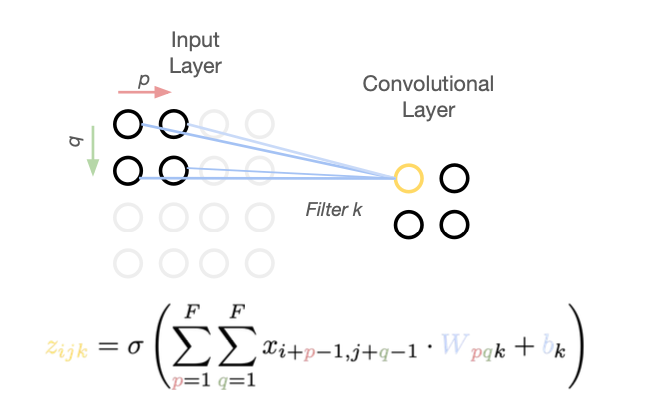
\includegraphics[width=1\textwidth]{img/4_conv.png}
    \caption{A diagram of a single convolutions filter acting on a single channel input with color- coded equation for demonstration purposes. The filter we display is two by two (or in general, $F \times F$ and the weight contributions (in blue) are multiplied by the input values (in black) and are summed over (red and green).
    }
\end{figure}

The convolutional layer is mathematically defined as:

\[
    z_{ijk} = \sigma \left( \sum_{p=1}^{F} \sum_{q=1}^{F} x_{i+p-1, j+q-1} \cdot W_{pqk} + b_k \right)
\]

Given an input \( \bm{x} \in \mathbb{R}^{H \times W \times C} \) (height \( H \), width \( W \), and \( C \) channels) and a set of \( K \) filters \( W_k \in \mathbb{R}^{F \times F \times C} \), the output feature map \( y \in \mathbb{R}^{H' \times W' \times K} \) is computed as:

\[
    y_{ijk} = \sigma \left( \sum_{c=1}^{C} \sum_{p=1}^{F} \sum_{q=1}^{F} x_{i+p-1, j+q-1, c} \cdot W_{pqck} + b_k \right)
\]

Here, \( \sigma \) is a non-linear activation function, and \( b_k \) is a bias term. The output dimensions \( H' \) and \( W' \) depend on the stride and padding used in the convolution operation. \marginnote[-100pt]{
    \noindent
    \textbf{Stride}: Stride refers to the step size with which the filter moves across the input. A larger stride reduces the spatial dimensions of the output.

    \bigskip

    \noindent
    \textbf{Padding}: Padding refers to the addition of extra pixels (typically zeros) around the input to control the output size. Padding ensures that the spatial dimensions of the input and output can be maintained or adjusted based on the chosen convolutional operation.
}

Convolutional layers are foundational in Convolutional Neural Networks (CNNs), which are widely used in tasks such as image classification, object detection, and segmentation.


\subsubsection{Recurrent Layers}

Recurrent layers are designed to handle sequential data (order of data points is important). These layers are the core components of Recurrent Neural Networks (RNNs), which are used in tasks such as time series prediction, natural language processing, and speech recognition. \bigskip

In a recurrent layer, the output at each time step depends on both the current input and the hidden state from the previous time step. This allows the network to maintain a memory of past inputs, capturing temporal dependencies.

\begin{figure}[h]
    \centering
    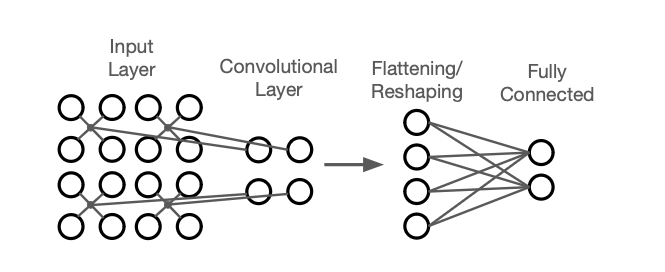
\includegraphics[width=1\textwidth]{img/4_fully_connected.png}
    \caption{A diagram of a simplistic neural network. The first layer is a convolution, followed by flattening and a fully connected layer representing the final output.}
\end{figure}

Formally, given an input sequence \( \bm{x} = [\bm{x_1}, \bm{x_2}, \dots, \bm{x_T}] \), the hidden state \( h_t \) at time step \( t \) is computed as:

\[
    h_t = \sigma \left( \bm{W}_h \bm{h}_{t-1} + \bm{W}_x \bm{x}_t + \bm{b}_h \right)
\]

where \( \bm{W}_h \) and \( \bm{W}_x \) are weight matrices, \( \bm{b}_h \) is a bias term, and \( \sigma \) is a non-linear activation function.


Variants such as Long Short-Term Memory (LSTM) networks and Gated Recurrent Units (GRUs) have been developed to address issues like vanishing gradients and to better capture long-term dependencies.


\subsubsection{Attention Layers}

Attention layers have revolutionised many areas of machine learning, particularly in natural language processing (NLP). The key idea behind attention mechanisms is to allow the model to focus on different parts of the input sequence when making predictions, rather than treating all parts of the sequence equally. This approach is a significant improvement to the model's ability to handle long sequences and complex dependencies.

\bigskip

A common type of attention mechanism is \textbf{self-attention}, where the model computes attention scores within a single sequence. Given an input sequence \( \bm{x} = [\bm{x}_1, \bm{x}_2, \dots, \bm{x}_T] \), the attention mechanism computes a set of output vectors \( \bm{y} = [\bm{y}_1, \bm{y}_2, \dots, \bm{y}_T] \) as:

\[
    \bm{y}_i = \sum_{j=1}^{T} \alpha_{ij} \bm{x}_j
\]

In this equation, \( \alpha_{ij} \) represents the attention weight that tells the model how much focus should be given to each input \( \bm{x}_j \) when generating the output \( \bm{y}_i \). The attention weights are computed using a compatibility function denoted by $a_\phi$.\bigskip

In the self-attention mechanism, the function \( a_\phi \) is used to compute the attention weights \( \alpha_{ij} \), which determine how much focus each input \( \bm{x}_j \) should receive when constructing the output \( \bm{y}_i \). \bigskip

The function \( a_\phi \) is called a compatibility function, as it measures how relevant or aligned two inputs \( \bm{x}_i \) and \( \bm{x}_j \) are. This compatibility score is then converted into a probability-like weight \( \alpha_{ij} \) through a softmax function.\bigskip

For example, in the commonly used \textbf{dot-product attention}, the function \( a_\phi \) is simply the dot product between two input vectors:
\[
    a_\phi(\bm{x}_i, \bm{x}_j) = \bm{x}_i^\top \bm{x}_j
\]
This gives a raw score of how similar or aligned \( \bm{x}_i \) and \( \bm{x}_j \) are. To compute the final attention weights \( \alpha_{ij} \), these scores are normalised across all inputs using a softmax function:
\begin{align*}
    \alpha_{ij} & = \frac{\exp(a_\phi(\bm{x}_i, \bm{x}_j))}{\sum_{k=1}^{T} \exp(a_\phi(\bm{x}_i, \bm{x}_k))}                     \\
                & = \frac{\exp \left( \bm{x}_i^\top \bm{x}_j \right)}{\sum_{k=1}^{T} \exp \left( \bm{x}_i^\top \bm{x}_k \right)}
\end{align*}

The process of computing attention scores and generating weighted sums for each output is visually depicted in Figure \ref{fig:attention}. This figure illustrates how each input vector \( \bm{e}_j \) is transformed through a function \( f_\psi \) before being scaled by attention weights \( \alpha_{ij} \). The weighted values are then summed to produce the output vector \( \bm{e}_j' \), demonstrating the flow of information in a self-attention layer.

\begin{figure}[h]
    \centering
    \begin{tikzpicture}

        \node (X1) {$\bm{x}_{1}$};
        \node[rectangle, right= 0.5em of X1] (x_dots_1) {$\dots$};
        \node[right=0.5em of x_dots_1] (Xj) {$\bm{x}_{j}$};
        \node[rectangle, right= 1em of Xj] (x_dots_2) {$\dots$};
        \node[right=1em of x_dots_2] (Xn) {$\bm{x}_{n}$};

        \node[rectangle, draw, ultra thick, above=of X1] (attn1) {\large $a_\phi$};
        \node[rectangle, draw, ultra thick, above=of Xj] (attnj) {\large $a_\phi$};
        \node[rectangle, draw, ultra thick, above=of Xn] (attnn) {\large $a_\phi$};

        \draw[-stealth, thick] (X1) -- (attn1);
        \draw[-stealth, thick] (Xj) -- (attn1);
        \draw[-stealth, thick] (Xj) -- (attnj);
        \draw[-stealth, thick] ([xshift=3em]Xj) -- (attnj);
        \draw[-stealth, thick] (Xj) -- (attnn);
        \draw[-stealth, thick] (Xn) -- (attnn);

        \node[above= of attn1, opacity=0.2] (alpha1j) {$\alpha_{1,j}$};
        \node[above= of attnj, opacity=1] (alphajj) {$\alpha_{j,j}$};
        \node[above= of attnn, opacity=0.6] (alphanj) {$\alpha_{n,j}$};

        \node[circle, draw, above=of alpha1j] (times1) {$\times$};
        \node[circle, draw, above=of alphajj] (timesj) {$\times$};
        \node[circle, draw, above=of alphanj] (timesn) {$\times$};

        \node[rectangle, draw, above=of timesj] (sum) {$\Sigma$};
        \node[above=1em of sum] (y_tprim) {$\bm{y}_i$};

        \draw[-stealth, line width=1.5mm, white] (attn1) -- (alpha1j);
        \draw[-stealth, thick, opacity=0.2] (attn1) -- (alpha1j);
        \draw[-stealth, line width=1.5mm, white] (attnj) -- (alphajj);
        \draw[-stealth, thick, opacity=1] (attnj) -- (alphajj);
        \draw[-stealth, line width=1.5mm, white] (attnn) -- (alphanj);
        \draw[-stealth, thick, opacity=0.6] (attnn) -- (alphanj);

        \draw[-stealth, white, line width=1.5mm] (X1) edge[bend right=30] (times1);
        \draw[-stealth, thick] (X1) edge[bend right=30] (times1);
        \draw[-stealth, white, line width=1.5mm] (Xj) edge[bend right=30] (timesj);
        \draw[-stealth, thick] (Xj) edge[bend right=30] (timesj);
        \draw[-stealth, thick] (Xn) edge[bend right=30] (timesn);

        \draw[-, line width=1.5mm, white] (times1) -- (sum);
        \draw[-stealth, thick] (times1) -- (sum);
        \draw[-, line width=1.5mm, white] (timesj) -- (sum);
        \draw[-stealth, thick] (timesj) -- (sum);
        \draw[-stealth, thick] (timesn) -- (sum);
        \draw[-stealth, thick] (times1) -- (sum);

        \draw[-stealth, line width=1.5mm, white] (alpha1j) -- (times1);
        \draw[-stealth, thick, opacity=0.2] (alpha1j) -- (times1);
        \draw[-stealth, line width=1.5mm, white] (alphajj) -- (timesj);
        \draw[-stealth, thick, opacity=1] (alphajj) -- (timesj);
        \draw[-stealth, line width=1.5mm, white] (alphanj) -- (timesn);
        \draw[-stealth, thick, opacity=0.6] (alphanj) -- (timesn);

        \draw[-stealth, thick] (sum) -- (y_tprim);

    \end{tikzpicture}
    \caption{Self-attention mechanism: Each input vector \( \bm{x}_j \) is weighted by attention weights \( \alpha_{ij} \) and then combined to form the output vector \( \bm{y}_i \).}
    \label{fig:attention}
\end{figure}


Self-attention is a key component of modern architectures like \textbf{Transformers} which rely heavily on this mechanism. Transformers have become state-of-the-art in many NLP tasks, such as machine translation, text generation, and question answering.


For more detailed readings, consider the seminal papers:
\begin{itemize}
    \item ``Convolutional Neural Networks for Visual Recognition" by Yann LeCun
    \item ``Long Short-Term Memory" by Hochreiter and Schmidhuber
    \item ``Attention is All You Need" by Vaswani et al.
\end{itemize}

\section{Automatic Differentiation}

In the context of Generalised Linear Models (GLMs), gradients are used for learning algorithms such as gradient descent.

\[\theta^{(t+1)}=\theta^{(t)}+\alpha\nabla_\theta\mathcal{L}(f^\theta,\bm{X},\bm{y})
\]

We will rewrite this as:

\[\theta^{(t+1)}=\theta^{(t)}-\alpha\nabla_\theta\mathcal{L}(\theta^{(t)})\]

It can sometimes be challenging to compute gradients manually. For neural networks, even small models can make manual gradient computation infeasible. To address this, we use a systematic approach called \textit{automatic differentiation}, which automates the process of computing derivatives.

\subsection{A Running Example}

Consider a one-hidden-layer neural network for regression:

\[
    \bm{z}^{(0)} = \bm{x}
\]
\[
    \zeta^{(1)} = \tanh\left( \bm{W}^{(1)} \bm{z}^{(0)} + \bm{b}^{(1)} \right)
\]
\[
    \bm{z}^{(2)} = \bm{W}^{(2)} \zeta^{(1)} + \bm{b}^{(2)}
\]

Assuming we have access to i.i.d. data samples, we aim to find parameters that minimise the loss function:
\[
    \mathcal{L}(\bm{y}, \bm{z}^{(2)}) = \left( \bm{y} - \bm{z}^{(2)} \right)^2
\]

To compute gradients such as \( \frac{\partial \mathcal{L}}{\partial \bm{W}^{(1)}} \), we would need to compute several intermediate derivatives.

\[\begin{aligned}
        \frac{\partial L}{\partial\boldsymbol{W}^{(1)}} & =\left(\frac{\partial L}{\partial\boldsymbol{z}^{(2)}}\cdot\frac{\partial\boldsymbol{z}^{(2)}}{\partial\zeta^{(1)}}\cdot\frac{\partial\zeta^{(1)}}{\partial(\boldsymbol{W}^{(1)}\boldsymbol{z}^{(0)}+\boldsymbol{b}^{(1)})}\right)\frac{\partial(\boldsymbol{W}^{(1)}\boldsymbol{z}^{(0)}+\boldsymbol{b}^{(1)})}{\partial\boldsymbol{W}^{(1)}} \\
                                                        & =\left((\boldsymbol{z}^{(2)}-\boldsymbol{y})^\top\boldsymbol{W}^{(2)}\circ\left(1-\tanh^2(\boldsymbol{W}^{(1)}\boldsymbol{z}^{(0)}+\boldsymbol{b}^{(1)})\right)\right)\boldsymbol{z}^{(0)\top}
    \end{aligned}\]

For small networks, manual computation may be feasible, but for deeper models, this process becomes impractical. Plus, everytime we make a minor modification we would need to re-derive our gradients. \bigskip

An alternative method to compute derivatives is the\textbf{ finite difference approach,} which approximates the derivative of a function \( f : \mathbb{R}^n \to \mathbb{R} \). For each input \( x_i \), the partial derivative can be approximated by:

\[
    \frac{\partial f}{\partial x_1} = \lim_{h \to 0} \frac{f(x_1 + h, x_2, \dots, x_n) - f(x_1, x_2, \dots, x_n)}{h}
\]
\[
    \frac{\partial f}{\partial x_2} = \lim_{h \to 0} \frac{f(x_1, x_2 + h, \dots, x_n) - f(x_1, x_2, \dots, x_n)}{h}
\]
\[
    \vdots
\]
\[
    \frac{\partial f}{\partial x_n} = \lim_{h \to 0} \frac{f(x_1, x_2, \dots, x_n + h) - f(x_1, x_2, \dots, x_n)}{h}
\]

The complexity of this method is $O(2nT)$, where $n$ is the number of parameters and $T$ is the complexity of evaluating the function or model once. We evaluate the function twice at $\bm{x}$ and $\bm{x} + (\bm{1} \cdot h)$ for $n$ parameters.\bigskip

However, applying this method to each parameter can be cumbersome and prone to compounded approximation errors, particularly in high-dimensional settings or complex functions.


\subsection{Introducing Automatic Differentiation}



The main concept of automatic differentiation is to break down complex equations into simpler operations, each of which can be easily differentiated. We can then apply the chain rule systematically. By understanding the sequence of operations, we can express the overall model as a composition of functions:
\[
    f(\bm{x}) = h(g(\bm{x}))
\]

\marginnote{

    \sns{Side Note on AutoDiff}{

        We are trying to compute $\alpha \nabla_{\theta} \mathcal{L}(\theta^{(t)})$ in
        \[
            \theta^{(t+1)} = \theta^{(t)} - \alpha \nabla_{\theta} \mathcal{L}(\theta^{(t)})
        \]
        \(\bm{J} := \nabla_{\theta} \mathcal{L}(\theta) \in \mathbb{R}^{m \times n}\),\\
        \(\theta^{(t)} \in \mathbb{R}^{n \times 1}\),\\
        \(\mathcal{L}(\theta) : \mathbb{R}^n \rightarrow \mathbb{R}^m\),\\
        \(\alpha > 0\),\\


    }

}

Previously, we sought an analytical expression for the Jacobian matrix, \( \nabla_x f \), to solve for optimal parameters. Consider two functions \( g: \mathbb{R}^n \to \mathbb{R}^k \) and \( h: \mathbb{R}^k \to \mathbb{R}^m \). By applying the chain rule, the Jacobian of the composed function is given by:

\[
    \bm{J}_f = \bm{J}_{h \circ g} = \bm{J}_h(g(\bm{x})) \bm{J}_g(\bm{x})
\]

This general principle allows us to compute \textbf{directional derivatives}, which are used to assemble gradients. Given a series of \( L \) compositions of functions, the directional derivative computed via automatic differentiation is:

\[
    \bm{J} \bm{x} = \bm{J}^{(L)} \bm{J}^{(L-1)} \dots \bm{J}^{(1)} \bm{x}
\]

Here, we are not computing the full Jacobian matrix, but rather the \textbf{Jacobian-vector product} with respect to the vector \( \bm{x} \), which is referred to as the \textbf{directional }derivative.

\subsection{Forward-Mode Automatic Differentiation}

The first paradigm of automatic differentiation we will cover is forward-mode. The key idea is that we compute the necessary derivatives of our function concurrently with the values during the forward pass. Forward mode can be viewed as breaking down the Jacobian-vector product in a sequential manner, as shown below:

\begin{align}
    \bm{J} \bm{x} & = \bm{J}^{(L)} \bm{J}^{(L-1)} \dots \bm{J}^{(1)} \bm{x} \notag                      \\
                  & = \bm{J}^{(L)} \bm{J}^{(L-1)} \dots \bm{J}^{(2)} (\bm{J}^{(1)} \bm{x}^{(1)}) \notag \\
                  & = \bm{J}^{(L)} \bm{J}^{(L-1)} \dots \bm{J}^{(3)} (\bm{J}^{(2)} \bm{x}^{(2)}) \notag \\
                  & \dots \notag                                                                        \\
    \bm{J} \bm{x} & = \bm{J}^{(L)} \bm{x}^{(L-1)} \label{eq:forward-mode-jacobian}
\end{align}


Here, \( \bm{x}^{(L-1)} \) denotes the intermediate result after the last Jacobian has been applied. \bigskip

Now, let us apply this process to a simple neural network model. In practice, when training neural networks, we aim to compute the gradient with respect to the parameters. However, to demonstrate the forward-mode process, we will compute the input gradient step by step. First, recall our example:

\[
    \bm{z}^{(0)} = \bm{x}
\]
\[
    \zeta^{(1)} = \tanh\left( \bm{W}^{(1)} \bm{z}^{(0)} + \bm{b}^{(1)} \right)
\]
\[
    \bm{z}^{(2)} = \bm{W}^{(2)} \zeta^{(1)} + \bm{b}^{(2)}
\]


Then, we express the forward pass and the loss function as a sequence of functions that we can program:

\begin{equation}
    \bm{z}^{(2)} = \text{Matmul}\left( \bm{W}^{(1)}, \tanh\left( \text{Matmul} \left( \bm{W}^{(0)} \bm{z}^{(0)} \right) \right) \right)
\end{equation}
\begin{equation}
    \mathcal{L} = \left( \bm{y} - \bm{z}^{(2)} \right)^2
\end{equation}

The purpose of this step is to identify the elementary operations involved in computing the loss, which will help us build the computational graph. \bigskip

In automatic differentiation literature, these operations are referred to as \textbf{primitives}. Each primitive represents a basic operation that is easy to differentiate. For example, the primitives we commonly deal with include functions like addition, multiplication, or applying activation functions (like \( \tanh \) or raising to a power). For each primitive, the differentiation rules from calculus apply.


\begin{figure}[ht]
    \centering
    \begin{tabularx}{\linewidth}{p{0.2\linewidth} p{0.2\linewidth} p{0.6\linewidth}}
        \toprule
        \textbf{Operation}               & \textbf{Value Update} & \textbf{Derivative Update}                                       \\
        \midrule
        Addition of a constant $c$       & $g(w) + c$            & $\frac{d}{dw}(g(w) + c) = \frac{d}{dw}g(w)$                      \\
        \hline
        Multiplication by a constant $c$ & $cg(w)$               & $\frac{d}{dw}(cg(w)) = c \frac{d}{dw}g(w)$                       \\
        \hline
        Raising to a power $n$           & $g(w)^n$              & $\frac{d}{dw}(g(w)^n) = n(g(w)^{n-1})\frac{d}{dw}g(w)$           \\
        \hline
        Applying Tanh                    & $\tanh(g(w))$         & $\frac{d}{dw}(\tanh(g(w))) = 1 - \tanh^2(g(w)) \frac{d}{dw}g(w)$ \\
        \bottomrule
    \end{tabularx}
    \caption{Value and Derivative Updates for Various Operations}
\end{figure}

Returning to our equations– we ignore the bias terms because they are relegated to affine basis expansion for brevity. We can now compute the forward pass and the derivative of the loss function, step by step:

\begin{align*}
    \bm{z}^{(0)} & = \bm{x}                                                                                                               \\
    \zeta^{(1)}  & = \tanh\left( \bm{W}^{(1)} \bm{z}^{(0)} + \bm{b}^{(1)} \right)                                                         \\
    \bm{z}^{(2)} & = \bm{W}^{(2)} \zeta^{(1)} + \bm{b}^{(2)}                                                                              \\
                 & = \text{Matmul}\left( \bm{W}^{(1)}, \tanh\left( \text{Matmul} \left( \bm{W}^{(0)} \bm{z}^{(0)} \right) \right) \right) \\
    \mathcal{L}  & = \left( \bm{y} - \bm{z}^{(2)} \right)^2
\end{align*}

\begin{figure}[h!]
    \centering
    \begin{tabularx}{\linewidth}{X X}
        \toprule
        \textbf{Value}      & \textbf{Derivative}          \\
        \midrule
        $x_0 = x$           & $d_0 = \bm{1}$               \\
        $x_1 = W^{(0)} x_0$ & $d_1 = W^{(0)\top} d_0$      \\
        $x_2 = \tanh(x_1)$  & $d_2 = 1 - \tanh^2(x_1) d_1$ \\
        $x_3 = W^{(1)} x_2$ & $d_3 = W^{(1)\top} d_2$      \\
        $x_4 = (y - x_3)$   & $d_4 = -d_3$                 \\
        $x_5 = (x_4)^2$     & $d_4 = 2(x_4) d_4$           \\
        \bottomrule
    \end{tabularx}
    \caption{Forward and Backward Pass for Value and Derivative Calculation. }
\end{figure}

\begin{figure}[h!]
    \centering
    \begin{tikzpicture}[>=Stealth, node distance=0.5cm, auto, scale=0.9, transform shape]
        % Define styles for nodes
        \tikzset{
            op/.style={rectangle, draw=black, fill=blue!20, thick, minimum size=8mm, rounded corners},
            var/.style={circle, draw=black, fill=yellow!30, thick, minimum size=8mm},
            arrow/.style={->, thick}
        }

        % Nodes for forward pass
        \node[var] (x0) {$x$};
        \node[var] (y) [below=of x0] {$y$};
        \node[op, right=of x0] (w0x0) {$\text{Matmul}\left(\bm{W}^{(0)} ( \cdot)\right)$};
        \node[var, right=of w0x0] (x1) {$x_1$};
        \node[op, right=of x1] (tanh1) {$\tanh(\cdot)$};
        \node[var, right=of tanh1] (x2) {$x_2$};
        \node[op, right=of x2] (w1x2) {$\text{Matmul}\left(\bm{W}^{(1)} ( \cdot)\right)$};
        \node[var, below=of w1x2] (x3) {$x_3$};
        \node[op, left=of x3] (sub) {$-$};
        \node[var, below=of sub] (x4) {$x_4$};
        \node[op, left=of x4] (square) {$(\cdot)^2$};
        \node[var, left=of square] (L) {$\mathcal{L}$};

        % Edges for forward pass
        \draw[arrow] (x0) -- (w0x0);
        \draw[arrow] (w0x0) -- (x1);
        \draw[arrow] (x1) -- (tanh1);
        \draw[arrow] (tanh1) -- (x2);
        \draw[arrow] (x2) -- (w1x2);
        \draw[arrow] (w1x2) -- (x3);
        \draw[arrow] (x3) -- (sub);
        \draw[arrow] (sub) -- (x4);
        \draw[arrow] (x4) -- (square);
        \draw[arrow] (square) -- (L);
        \draw[arrow] (y) -- (sub);

        % % Backward pass (derivatives)
        % \node[var, below=3.0cm of w1x2, ] (d4) {$d_4$};
        % \node[op, left=of d4] (subd3) {$-$};
        % \node[var, left=of subd3] (d3) {$d_3$};
        % \node[op, left=of d3] (tanhd2) {$1-\tanh^2$};
        % \node[var, left=of tanhd2] (d2) {$d_2$};
        % \node[op, left=of d2] (w0td1) {$W^{(0)\top}$};
        % \node[var, left=of w0td1] (d1) {$d_1$};
        % \node[op, left=of d1] (loss) {Loss};

        % % Edges for backward pass
        % \draw[arrow] (d4) -- (subd3);
        % \draw[arrow] (subd3) -- (d3);
        % \draw[arrow] (d3) -- (tanhd2);
        % \draw[arrow] (tanhd2) -- (d2);
        % \draw[arrow] (d2) -- (w0td1);
        % \draw[arrow] (w0td1) -- (d1);
        % \draw[arrow] (d1) -- (loss);
    \end{tikzpicture}
    \caption{Computational Graph for the example neural network.}
\end{figure}

For an example $x = 1$, $W^{(0)} = 2$, $W^{(1)} = 1.2$, $y = 2$, the calculations would look like the following:
\begin{figure}[h!]
    \centering
    \begin{tabularx}{\linewidth}{p{0.4\linewidth} p{0.6\linewidth}}
        \toprule
        \textbf{Value}                                                & \textbf{Derivative}                                                   \\
        \midrule
        $x_0 = x \Rightarrow 1$                                       & $d_0 = \bm{1}$                                                        \\
        $x_1 = W^{(0)} x_0 \Rightarrow 1 \times 2 = 2$                & $d_1 = W^{(0)\top} d_0 \Rightarrow 2 \times d_0 = 2$                  \\
        $x_2 = \tanh(x_1) \Rightarrow \tanh(2) \approx 0.964$         & $d_2 = (1 - \tanh^2(2)) d_1 \Rightarrow 0.14 \times d_1 \approx 0.14$ \\
        $x_3 = W^{(1)} x_2 \Rightarrow 1.2 \times 0.964 \approx 1.15$ & $d_3 = W^{(1)\top} d_2 \Rightarrow 1.2 \times 0.14 \approx 0.169$     \\
        $x_4 = y - x_3 \Rightarrow 2 - 1.15 = 0.85$                   & $d_4 = -d_3 \Rightarrow -0.169$                                       \\
        $x_5 = (x_4)^2 \Rightarrow (0.85)^2 = 0.722$                  & $d_5 = 2(x_4) d_4 \Rightarrow 2(0.85) \times (-0.169) \approx -0.283$ \\
        \bottomrule
    \end{tabularx}
    \caption{Forward and Backward Pass for Value and Derivative Calculation with extensions.}
\end{figure}


To clarify, \( \bm{x}_0 \) is the input, \( \bm{x}_1 \) is the result of the first matrix multiplication, \( \bm{x}_2 \) is after applying the activation function, \( \bm{x}_3 \) is the second matrix multiplication, \( \bm{x}_4 \) represents the absolute error with respect to the label, and \( \bm{x}_5 \) is the squared error. We computed \( d_5 = \frac{d \mathcal{L}}{d \bm{x}} = -0.283 \), but this does not provide \( \frac{d \mathcal{L}}{d \bm{W}^{(1)}} \). To compute this, another forward differentiation would be needed, which is beyond this example.


\subsection{Complexity of Forward Mode Differentiation}

Let the forward pass complexity be $T$, the number of operations required to compute the function. The computational complexity of finding the Jacobian with forward mode automatic differentiation is $O(2nT)$. This is identical to the complexity of finite-difference approximation, but a much less approximation error since approximations are not compounded.

\subsection{Reverse-Mode Automatic Differentiation}

The idea of reverse mode is to begin with an output and propagate backwards, rather than beginning with an input and propagating forwards. This is particularly useful when the number of inputs is much larger than the number of outputs, as is the case with neural networks. \bigskip

In forward-mode automatic differentiation (AD), we track both the nominal values and the tangents (directional derivatives). We could do this by using the associativity of matrix products that give us our Jacobian matrix, as in Equation \ref{eq:forward-mode-jacobian}. \bigskip

Reverse-mode AD, however, focuses on computing adjoints, which can be defined as:
\[
    \bar{x} = \frac{\partial z}{\partial x}
\]

\defb{`Adjoint' in Automatic Differentiation (AD)}{
    `Adjoint' comes from linear algebra, and in the context of automatic differentiation (AD), particuarly reverse-mode AD, it refers to the propagation of derivatives. \bigskip

    The adjoint of a variable $x$ is the derivative of the target function (often the loss function in ML) with respect to $x$. It is framed towards the reverse accumulation of derivatives in a system.


    \[
        \bar{x} = \frac{\partial z}{\partial x}
    \]
}

This adjoint must have the correct shape to be multiplied by the Jacobian. To illustrate, consider the output of a model, \( \bm{y} - f(\bm{x}) \), and compute the derivative in reverse order with respect to the output:



\begin{align*}
    \bm{Jx} = \bar{\bm{y}} \bm{J} & = (\bar{\bm{y}} \bm{J}^{(L)}) \bm{J}^{(L-1)} \dots \bm{J}^{(1)}           \\
                                  & = (\bar{\bm{y}}^{(L)} \bm{J}^{(L-1)}) \bm{J}^{(L-2)} \dots \bm{J}^{(1)}   \\
                                  & = (\bar{\bm{y}}^{(L-1)} \bm{J}^{(L-2)}) \bm{J}^{(L-3)} \dots \bm{J}^{(1)} \\
                                  & \dots                                                                     \\
                                  & = \bar{\bm{y}}^{(2)} \bm{J}^{(1)}
\end{align*}

\marginnote[-80pt]{

    \sns{Side Note on AutoDiff}{

        We are trying to compute $\alpha \nabla_{\theta} \mathcal{L}(\theta^{(t)})$ in
        \[
            \theta^{(t+1)} = \theta^{(t)} - \alpha \nabla_{\theta} \mathcal{L}(\theta^{(t)})
        \]
        \(\bm{J} := \nabla_{\theta} \mathcal{L}(\theta) \in \mathbb{R}^{m \times n}\),\\
        \(\theta^{(t)} \in \mathbb{R}^{n \times 1}\),\\
        \(\mathcal{L}(\theta) : \mathbb{R}^n \rightarrow \mathbb{R}^m\),\\
        \(\alpha > 0\),\\


    }

    In contrast to Forward Mode:

    \begin{align*}
        \bm{J} \bm{x} & = \bm{J}^{(L)} \bm{J}^{(L-1)} \dots \bm{J}^{(1)} \bm{x}                      \\
                      & = \bm{J}^{(L)} \bm{J}^{(L-1)} \dots \bm{J}^{(2)} (\bm{J}^{(1)} \bm{x}^{(1)}) \\
                      & = \bm{J}^{(L)} \bm{J}^{(L-1)} \dots \bm{J}^{(3)} (\bm{J}^{(2)} \bm{x}^{(2)}) \\
                      & \dots                                                                        \\
        \bm{J} \bm{x} & = \bm{J}^{(L)} \bm{x}^{(L-1)}
    \end{align*}

}



In reverse mode, we compute the necessary Jacobians in reverse order, meaning we need intermediate results from the forward pass. For a fully connected neural network with \( L \) layers, the forward pass is given by:

\begin{align*}
    \bm{z}^{(1)}   & = \bm{x}                                                        \\
    \bm{z}^{(i+1)} & = \sigma\left( \bm{W}^{(i)} \bm{z}^{(i)} + \bm{b}^{(i)} \right)
\end{align*}

Now, let us consider the weights and biases to be joined into parameters denoted \( \theta^{(i)} = \{ \bm{W}^{(i)}, \bm{b}^{(i)} \} \). We aim to compute the gradient of our function starting from the last layer using the chain rule:

\begin{align*}
    \frac{\partial \mathcal{L}}{\partial \theta^{(L-1)}} & = \frac{\partial \mathcal{L}}{\partial \bm{z}^{(L)}} \textcolor{blue}{\frac{\partial \bm{z}^{(L)}}{\partial \theta^{(L-1)}}}                                                                                                                                                                                                                \\
    \frac{\partial \mathcal{L}}{\partial \theta^{(L-2)}} & = \frac{\partial \mathcal{L}}{\partial \bm{z}^{(L)}} \textcolor{orange}{\frac{\partial \bm{z}^{(L)}}{\partial \bm{z}^{(L-1)}}} \textcolor{blue}{\frac{\partial \bm{z}^{(L-1)}}{\partial \theta^{(L-2)}}}                                                                                                                                    \\
    \frac{\partial \mathcal{L}}{\partial \theta^{(L-3)}} & = \frac{\partial \mathcal{L}}{\partial \bm{z}^{(L)}} \textcolor{orange}{\frac{\partial \bm{z}^{(L)}}{\partial \bm{z}^{(L-1)}} \frac{\partial \bm{z}^{(L-1)}}{\partial \bm{z}^{(L-2)}} } \textcolor{blue}{\frac{\partial \bm{z}^{(1)}}{\partial \theta^{(L-3)}}}                                                                             \\
    \frac{\partial \mathcal{L}}{\partial \theta^{(i)}}   & = \frac{\partial \mathcal{L}}{\partial \bm{z}^{(L)}} \textcolor{orange}{\frac{\partial \bm{z}^{(L)}}{\partial \bm{z}^{(L-1)}} \frac{\partial \bm{z}^{(L-1)}}{\partial \bm{z}^{(L-2)}} } \dots \textcolor{orange}{\frac{\partial \bm{z}^{(2)}}{\partial \bm{z}^{(1)}}} \textcolor{blue}{\frac{\partial \bm{z}^{(1)}}{\partial \theta^{(i)}}}
\end{align*}

We can observe that by chain rule, we can compute the partial derivative of the parameters in layer $i$ by computing the \textcolor{orange}{partial derivative of the layer w.r.t its input}, and then multiply it with the \textcolor{blue}{partial derivative of the layer output w.r.t its parameters}. Using this recursive application of the chain rule, we propagate the error back through the layers, computing the gradient of the loss \( \mathcal{L} \) with respect to each parameter \( \theta^{(i)} \).

\newpage
\subsection{General Adjoint/Reverse Mode Algorithm}

We now describe the general reverse-mode automatic differentiation algorithm. Let \( x_1, x_2, \dots, x_D \) be the input variables, and \( x_{d+1}, \dots, x_{D-1} \) be the intermediate variables, with \( x_D \) as the output variable. The flow of the computational graph is given by: \marginnote{
    We are trying to avoid graph theory notation as much as possible in the notes.
}

\begin{equation}
    x_i = g_i(x_{\text{Pa}(x_i)})
    \quad \forall i \in [d+1, D]
\end{equation}

Here, \( g_i \) is the elementary operation associated with the node in the graph, and \( \text{Pa}(x_i) \) is the function that returns the set of parent (incoming) nodes to variable \( x_i \).


\begin{figure}[h!]
    \centering
    \begin{tikzpicture}[>=Stealth, node distance=0.5cm, auto, scale=0.9, transform shape]
        % Define styles for nodes
        \tikzset{
            op/.style={rectangle, draw=black, fill=blue!20, thick, minimum size=13mm, rounded corners},
            var/.style={circle, draw=black, fill=yellow!30, thick, minimum size=13mm},
            arrow/.style={->, thick}
        }

        % Input Nodes
        \node[var] (x1) {$x_1$};
        \node[var, below= of x1] (x2) {$x_2$};
        \node[draw=none, below= of x2] (xdots) {$\vdots$};
        \node[var, below= of xdots] (xd) {$x_d$};

        % Operations
        \node[op, right=of x1] (gd1) {$g_{d+1}$};
        \node[op, right=of x2] (gd2) {$g_{d+2}$};
        \node[draw=none, below=of gd2] (xdots) {$\vdots$};


        % Intermediate Nodes
        \node[var, right=of gd1] (xd1) {$x_{d+1}$};
        \node[var, right=of gd2] (xd2) {$x_{d+2}$};
        \node[draw=none, below=of xd2] (xdots) {$\vdots$};

        % Operations
        \node[op, right=2cm of xd1] (gd3) {$g_{D}$};
        \node[draw=none, right=of xd1, yshift=0.1cm] (gdots) {$\cdots$};

        % Last Nodes
        \node[var, right=of gd3] (xD) {$x_{D}$};


        % Intermediate and output nodes
        % Output node
        % \node[var, right=of g4] (output) {$f$};

        \draw[arrow] (x1) -- (gd1.west);
        \draw[arrow] (x2) -- (gd2.west);
        \draw[arrow] (xd) -- (gd1.west);

        \draw[arrow] (xd) -- (gd2.west);

        \draw[arrow] (gd1) -- (xd1.west);
        \draw[arrow] (gd2) -- (xd2.west);

        \draw[arrow] (xd1) -- (gd3.west);
        \draw[arrow] (xd2) -- (gd3.west);

        \draw[arrow] (xd) to[bend right] (gd3.south);
        \draw[arrow] (gd3) -- (xD.west);






    \end{tikzpicture}
    \caption{Computational Graph notation}
\end{figure}


The chain rule can then be applied to compute the derivative:

\begin{equation}
    \frac{\partial f}{\partial x_i} = \sum_{x_j : i \in \text{Pa}(x_j)} \frac{\partial x_j}{\partial x_i} \frac{\partial f}{\partial x_j} = \sum_{x_j : i \in \text{Pa}(x_j)} \frac{\partial g_j}{\partial x_i} \frac{\partial f}{\partial x_j} \label{eq:reverse-mode-chain-rule}
\end{equation}



\ex{Example of finding the computational graph}{
Consider the function:

\[
    f(x) = \sqrt{x^2 + \exp(x^2)} + \cos\left( x^2 + \exp(x^2) \right)
\]

We break this equation down into its elementary operations: { square root, exponential, power, cosine, addition }:

\begin{align*}
    x_1 & = x^2 \quad        & \frac{\partial x_1}{\partial x}   & = 2x                                   \\
    x_2 & = \exp(x_1) \quad  & \frac{\partial x_2}{\partial x_1} & = \exp(x_1)                            \\
    x_3 & = x_1 + x_2 \quad  & \frac{\partial x_3}{\partial x_1} & =\frac{\partial x_3}{\partial x_2} = 1 \\
    x_4 & = \sqrt{x_3} \quad & \frac{\partial x_4}{\partial x_3} & = \frac{1}{2\sqrt{x_3}}                \\
    x_5 & = \cos(x_3) \quad  & \frac{\partial x_5}{\partial x_3} & = -\sin(x_3)                           \\
    x_6 & = x_4 + x_5 \quad  & \frac{\partial x_6}{\partial x_4} & =\frac{\partial x_6}{\partial x_5} = 1
\end{align*}

Here, \( x_6 \) represents the complete function \( f(z) \). Before performing the backward pass, it is useful to write out the derivative of each function at each step.

\begin{center}
    \begin{tikzpicture}[>=Stealth, node distance=0.5cm, auto, scale=0.85, transform shape]
        % Define styles for nodes
        \tikzset{
            op/.style={rectangle, draw=black, fill=blue!20, thick, minimum size=8mm, rounded corners},
            var/.style={circle, draw=black, fill=yellow!30, thick, minimum size=8mm},
            arrow/.style={->, thick}
        }

        % Nodes for the graph
        \node[var] (x) {$x$};
        \node[op, right=of x] (square) {$(\cdot)^2$};
        \node[var, right=of square] (a) {$x_1$};
        \node[op, above right=of a] (exp) {exp$(\cdot)$};
        \node[var, right=of exp] (b) {$x_2$};
        \node[op, below right=of b] (plus1) {$+$};
        \node[var, right=of plus1] (c) {$x_3$};
        \node[op, above right=of c] (sqrt) {$\sqrt{\cdot}$};
        \node[var, right=of sqrt] (d) {$x_4$};
        \node[op, below right=of c] (cos) {cos$(\cdot)$};
        \node[var, right=of cos] (e) {$x_5$};
        \node[op, below right=of d] (plus2) {$+$};
        \node[var, right=of plus2] (f) {$f$};

        % Edges for the graph
        \draw[arrow] (x) -- (square);
        \draw[arrow] (square) -- (a);
        \draw[arrow] (a) to[bend left] (exp.west);
        \draw[arrow] (exp.east) -- (b);
        \draw[arrow] (b) to[bend left] (plus1.north);
        \draw[arrow] (a) -- (plus1);
        \draw[arrow] (plus1) -- (c);
        \draw[arrow] (c) to[bend left] (sqrt.west);
        \draw[arrow] (sqrt) -- (d);
        \draw[arrow] (d) to[bend left] (plus2.north);
        \draw[arrow] (c) to[bend right] (cos.west);
        \draw[arrow] (cos) -- (e);
        \draw[arrow] (e) to[bend right] (plus2.south);
        \draw[arrow] (plus2) -- (f);


    \end{tikzpicture}
\end{center}

Now that we have defined the derivatives, we can construct a computational graph by working backwards from the output. The chain rule is applied step by step:

\begin{align*}
    \frac{\partial x_6}{\partial x_3} & = \frac{\partial x_6}{\partial x_4} \frac{\partial x_4}{\partial x_3} + \frac{\partial x_6}{\partial x_5} \frac{\partial x_5}{\partial x_3} \\
    \frac{\partial x_6}{\partial x_2} & = \frac{\partial x_6}{\partial x_3} \frac{\partial x_3}{\partial x_2}                                                                       \\
    \frac{\partial x_6}{\partial x_1} & = \frac{\partial x_6}{\partial x_2} \frac{\partial x_2}{\partial x_1} + \frac{\partial x_6}{\partial x_3} \frac{\partial x_3}{\partial x_1} \\
    \frac{\partial x_6}{\partial x}   & = \frac{\partial x_6}{\partial x_1} \frac{\partial x_1}{\partial x}
\end{align*}

While working backwards, ensure all parent nodes are accounted for (summed) to avoid incorrect partial derivatives. Though we only derive the recipe for the derivative and not the actual values, understanding the process outlined in Equations \ref{eq:forward-mode-jacobian} is important.



}

\subsection{Complexity of Reverse Mode Differentiation}
\begin{itemize}
    \item The function must be evaluated once(forward pass) to get the output, in order to compute all the intermediate values. This has complexity $T$.
    \item The function must be evaluated (with complexity $T$) for each of the $m$ outputs.
    \item We get $O(mT + T)$. In many cases, $m$ is much smaller than the number of inputs, so reverse mode (with complexity $O(mT+T)$) is more efficient than forward mode (with complexity $O(2nT)$).
\end{itemize}

\chapter{Convexity, Convergence and Optimisation}


\refb{Additional Resources}{
    \begin{itemize}
        \item Covering basic ideas: \textit{Numerical Computation}, Chapter 4 (Page 78) Bengio et al. (2017)

        \item Practical but introductory discussion of gradient descent in deep models, Chapter 8 (Page 271) Bengio et al. (2017)

        \item More comprehensive overall coverage: \textit{Continuous Optimization}, Chapter 7 (Page 225) up to 7.4 Deisenroth et al. (2020)
    \end{itemize}

}


\section{Learning as Optimisation}

In previous lectures, we explored gradient descent as a method for finding the optimal parameter for a given model and dataset. In this lecture, we will delve deeper into this process by revisiting the optimisation problem we aim to solve:

\[
    \theta^* = \arg\min_{\theta} \frac{1}{N} \sum_{i}^N \mathcal{L}(f^\theta(\bm{x}^{(i)}), \bm{y}^{(i)})
\]

Here, $\theta^*$ is referred to as the optimal parameter. The argmin operator returns the parameter value that minimises the following loss function:

\[
    \min_{\theta} \frac{1}{N} \sum_{i}^N \mathcal{L}(f^\theta(\bm{x}^{(i)}), \bm{y}^{(i)})
\]

The core algorithm used to solve this minimisation problem is gradient descent, which we previously introduced. The algorithm, stated both in practical and mathematical terms, is as follows:



\begin{algorithm}
    \caption{Gradient Descent}\label{alg:gradient_descent}
    \textbf{Input: } $X$ - Inputs, $Y$ - Labels, $\alpha$ - Learning rate, $K$ - Number of iterations
    \vspace{-8pt} % stupid hack for tufte book
    \par\noindent\rule{\linewidth}{0.5pt}
    \vspace{-15pt} % stupid hack for tufte book
    \begin{algorithmic}[1]
        \State $\theta^{(1)} \gets \text{Random Initialisation}$
        \For{$i \in [K]$}
        \State $l \gets \mathcal{L}(Y, f^\theta(X))$
        \State $\theta^{(i+1)} \gets \theta^{(i)} - \alpha \nabla_{\theta} l$
        \EndFor
        \State \Return $\theta_K$
    \end{algorithmic}
\end{algorithm}


Gradient descent iteratively updates the parameter $\theta$ using the gradient of the loss function, scaled by the learning rate $\alpha$, until convergence or after $K$ iterations.

\newpage
\section{Progress Bounds for Gradient Descent}

Given our understanding of gradient descent, we have:

\[
    \theta^{(t+1)} = \theta^{(t)} - \alpha \nabla \mathcal{L}(\theta^{(t)})
\]
\begin{itemize}[noitemsep]
    \item \(\mathcal{L}(\theta) : \mathbb{R}^n \rightarrow \mathbb{R}^m\),
    \item \(\nabla_{\theta} \mathcal{L}(\theta) \in \mathbb{R}^{m \times n}\),
    \item \(\alpha > 0\),
    \item \(\bm{J} := \nabla_{\theta} \mathcal{L}(\theta)\) (Jacobian matrix).
\end{itemize}



One critical question about gradient descent is: \textit{does it work}? While practical experiments have established it as a de facto workhorse in machine learning, we will use mathematical tools to understand why and when it works. To do this, we assume that the function is \textbf{Lipschitz Continuous}.

\defb{Lipschitz Continuous Gradient}{
    A function $\mathcal{L}(\theta) : \mathbb{R}^n \rightarrow \mathbb{R}$ has a Lipschitz continuous gradient if there exists a constant $L > 0$ such that for all $\bm{u}, \bm{v} \in \mathbb{R}^n$, the following inequality holds:
    \[
        \|\nabla \mathcal{L}(\bm{u}) - \nabla \mathcal{L}(\bm{v})\| \leq L \|\bm{u} - \bm{v}\|.
    \]
    The constant $L$ is called the Lipschitz constant, which bounds the rate of change of the gradient.\bigskip
}

\defb{Showing \ensuremath{L \geq \|H(\bm{v})\|}}{
    For any twice-differentiable function, by Lipschitz continuity, it can be shown that
    \[
        L \geq \|H(\bm{v})\|
    \]

    To show this, rewrite the second line assumption of Lipschitz continuity as
    \[
        L \geq \frac{\|\nabla \mathcal{L}(\bm{w}) - \nabla \mathcal{L}(\bm{v})\|}{\|\bm{w} - \bm{v}\|}
    \]

    We return to the Taylor Expansion and differentiate again:
    \begin{align*}
        \mathcal{L}(\bm{w})        & \approx \mathcal{L}(\bm{v}) + \nabla \mathcal{L}(\bm{v})^\top (\bm{w} - \bm{v}) + \frac{1}{2} (\bm{w} - \bm{v})^\top H(\bm{v})(\bm{w} - \bm{v}) \\
        \nabla \mathcal{L}(\bm{w}) & = \nabla \mathcal{L}(\bm{v}) + H(\bm{v})(\bm{w} - \bm{v}) + o(\|\bm{w} - \bm{v}\|)
    \end{align*}
    \begin{align*}
        \nabla \mathcal{L}(\bm{w}) - \nabla \mathcal{L}(\bm{v})                                 & \geq H(\bm{v})(\bm{w} - \bm{v})                                    \\
        \frac{\nabla \mathcal{L}(\bm{w}) - \nabla \mathcal{L}(\bm{v})}{\|\bm{w} - \bm{v}\|}     & \geq \frac{H(\bm{v})(\bm{w} - \bm{v})}{\|\bm{w} - \bm{v}\|}        \\
        \frac{\|\nabla \mathcal{L}(\bm{w}) - \nabla \mathcal{L}(\bm{v})\|}{\|\bm{w} - \bm{v}\|} & \geq \|H(\bm{v})\| \frac{\|\bm{w} - \bm{v}\|}{\|\bm{w} - \bm{v}\|}
    \end{align*}

    Rearranging the rewritten Lipschitz continuity assumption into the equation, we have
    \[
        L \geq \frac{\|\nabla \mathcal{L}(\bm{w}) - \nabla \mathcal{L}(\bm{v})\|}{\|\bm{w} - \bm{v}\|} \geq \|H(\bm{v})\|
    \]
    Where \( \bm{u} \) is the unit norm with \( \|\bm{u}\| = 1 \), giving us
    \[
        L \geq \|H(\bm{v})\|
    \]
}


\subsection{Proving Gradient Descent Minimises \ensuremath{\mathcal{L}} per step}

For a twice-differentiable function $\mathcal{L}(\theta)$, we can expand it around a point $\bm{\theta_0}$ using a multivariate Taylor expansion. Given two points $\bm{v}$ and $\bm{w} \in \mathbb{R}^n$, we have:
\[
    \mathcal{L}(\bm{w}) \approx \mathcal{L}(\bm{v}) + \nabla \mathcal{L}(\bm{v})^\top (\bm{w} - \bm{v}) + \frac{1}{2} (\bm{w} - \bm{v})^\top H(\bm{v})(\bm{w} - \bm{v}),
\]
where $H(\bm{v})$ is the Hessian matrix of $\mathcal{L}$ at $\bm{v}$.\bigskip

By assuming that the gradient of $\mathcal{L}$ is Lipschitz continuous with constant $L$, it can be shown $L \geq \|H(\bm{v})\|$, so we can bound the second-order term, giving:
\[
    \mathcal{L}(\bm{w}) \leq \mathcal{L}(\bm{v}) + \nabla \mathcal{L}(\bm{v})^\top (\bm{w} - \bm{v}) + \frac{L}{2} \|\bm{w} - \bm{v}\|^2.
\]
This inequality is known as the \textit{descent lemma}, which provides an upper bound on the function value in terms of the gradient and the Lipschitz constant.

Recalling the gradient descent update rule, where at iteration \(t\) we update the parameter \(\theta\) as follows:
\[
    \theta^{(t+1)} = \theta^{(t)} - \alpha \nabla \mathcal{L}(\theta^{(t)}),
\]
we subtract \(\theta^{(t)}\) from both sides to get:
\[
    \theta^{(t+1)} - \theta^{(t)} = -\alpha \nabla \mathcal{L}(\theta^{(t)}).
\]

Recall the gradient descent lemma– we then substitute $\mathcal{L}(\bm{w})$ with $\mathcal{L}(\theta^{(t+1)})$ and $\mathcal{L}(\bm{v})$ with $\mathcal{L}(\theta^{(t)})$:
\[
    \mathcal{L}(\bm{w}) \leq \mathcal{L}(\bm{v}) + \nabla \mathcal{L}(\bm{v})^\top (\bm{w} - \bm{v}) + \frac{L}{2} \|\bm{w} - \bm{v}\|^2.
\]

We have:
\[
    \mathcal{L}(\theta^{(t+1)})\leq\mathcal{L}(\theta^{(t)})+\nabla\mathcal{L}(\theta^{(t)})^\top(\theta^{(t+1)}-\theta^{(t)})+\frac L2\left\|\theta^{(t+1)}-\theta^{(t)}\right\|^2
\]

We then substitute the first occurence of $\theta^{(t+1)} - \theta^{(t)}$ with $-\alpha \nabla \mathcal{L}(\theta^{(t)})$:

\[
    \mathcal{L}(\theta^{(t+1)}) \leq \mathcal{L}(\theta^{(t)}) - \nabla \mathcal{L}(\theta^{(t)})^\top (\alpha \nabla \mathcal{L}(\theta^{(t)})) + \frac L2\left\|\theta^{(t+1)}-\theta^{(t)}\right\|^2
\]

Let $\alpha = \frac{1}{L}$, then we have:

\[
    \mathcal{L}(\theta^{(t+1)})\leq\mathcal{L}(\theta^{(t)})-\frac1L\|\nabla\mathcal{L}(\theta^{(t)})\|^2+\frac L2\left\|\theta^{(t+1)}-\theta^{(t)}\right\|^2
\]


where \(\|\theta^{(t+1)} - \theta^{(t)}\| = \frac{1}{L} \|\nabla \mathcal{L}(\theta^{(t)})\|\), we obtain:
\[
    \mathcal{L}(\theta^{(t+1)}) \leq \mathcal{L}(\theta^{(t)}) - \frac{1}{2L} \|\nabla \mathcal{L}(\theta^{(t)})\|^2.
\]
This shows that the function value decreases by at least \(\frac{1}{2L} \|\nabla \mathcal{L}(\theta^{(t)})\|^2\) at each step, proving that gradient descent makes progress towards minimising \(\mathcal{L}\).
\hfill\(\Box\)

\section{Convex Optimisation}

We have shown of gradient descent moves us in a direction that improves the loss of our model. But as we continue in that direction, where will we end up? We begin answering this question by considering \textbf{convex optimisation}. \bigskip

An optimisation problem is convex if and only if the function we are optimising is convex and the domain of the problem is convex. For a function to be convex, it must satisfy:

\defb{Definition 5.3.1. Convex Function}{
We say that a function \(\mathcal{L}(\theta) : \mathbb{R}^n \rightarrow \mathbb{R}\) is convex if and only if:
\[
\mathcal{L}(\alpha \theta + (1 - \alpha) \theta') \leq \alpha \mathcal{L}(\theta) + (1 - \alpha) \mathcal{L}(\theta')
\]
This definition is formulated in terms of the secant of a function and essentially says that every function value between \(\mathcal{L}(\theta)\) and \(\mathcal{L}(\theta')\) must lie below or on the secant. We also require that the domain of the function is a convex set.
\begin{center}


    \begin{tikzpicture}[scale=1, domain=0:4.5]

        % Define points on the x-axis
        \coordinate (theta) at (0.4, 0);   % \theta
        \coordinate (theta_prime) at (4, 0);    % \theta'
        \coordinate (alpha_theta) at (2.3, 0); % Interpolated \alpha \theta + (1-\alpha)\theta'
        \coordinate (y1) at (0,2.28);
        \coordinate (y2) at (0,3);

        % Define corresponding points on the y-axis (\mathcal{L}(\theta), \mathcal{L}(\theta')) and the interpolated y-point
        \coordinate (L_theta) at (0.4, 2.28);  % \mathcal{L}(\theta)
        \coordinate (L_theta_prime) at (4, 3);   % \mathcal{L}(\theta')
        \coordinate (L_alpha) at (2.3, 2.64); % Interpolated \alpha \mathcal{L}(\theta) + (1-\alpha) \mathcal{L}(\theta')

        % Label \theta, \theta', and the interpolated point on the x-axis
        \node[below] at (theta) {$\theta$};
        \node[below] at (theta_prime) {$\theta'$};
        \node[below] at (alpha_theta) {$\alpha \theta + (1-\alpha) \theta'$};

        % Label \mathcal{L}(\theta) and \mathcal{L}(\theta') on the y-axis
        \node[left] at (0, 2.28) {$\mathcal{L}(\theta)$};
        \node[left] at (0, 3) {$\mathcal{L}(\theta')$};

        % Label the interpolated point on the secant line (position the label on top and higher)
        \node[right, xshift=1.7cm, text=red] at (L_alpha) {\textcolor{red}{$\alpha \mathcal{L}(\theta) + (1-\alpha) \mathcal{L}(\theta')$}};


        % Draw axes
        \draw[thick,->] (-0.5,0) -- (5,0) node[right] {$\theta$};   % x-axis
        \draw[thick,->] (0,-0.5) -- (0,5.0) node[above] {$\mathcal{L}$};   % y-axis

        % Draw convex function \mathcal{L}(\theta) = 0.5\theta^2 - 2\theta + 3
        \draw[thick,blue,domain=-0.5:4.5,samples=100] plot (\x, {0.5*(\x)*(\x) - 2*(\x) + 3}) node[right] {$\mathcal{L}(\theta)$};

        % Mark points on the convex function
        \fill (L_theta) circle (1pt);  % \mathcal{L}(\theta)
        \fill (L_theta_prime) circle (1pt);  % \mathcal{L}(\theta')

        % Draw secant line (line between the two points on the curve)
        \draw[thick, magenta] (L_theta) -- (L_theta_prime);

        % Draw dashed lines from \theta and \theta' to the corresponding function points
        \draw[dashed] (theta) -- (L_theta);  % Dashed line from \theta to \mathcal{L}(\theta)
        \draw[dashed] (theta_prime) -- (L_theta_prime);  % Dashed line from \theta' to \mathcal{L}(\theta')

        % Draw dashed lines from the function values to the y-axis
        \draw[dashed] (y1) -- (L_theta);  % Dashed line from y-axis to \mathcal{L}(\theta)
        \draw[dashed] (y2) -- (L_theta_prime);  % Dashed line from y-axis to \mathcal{L}(\theta')

        % Mark the interpolated point on the secant line
        \fill (L_alpha) circle (1pt);

        % Draw the interpolated point to the x and y axes
        \draw[dashed] (alpha_theta) -- (L_alpha);  % Dashed line from alpha_theta to L_alpha

    \end{tikzpicture}



\end{center}
}

\defb{Definition 5.3.2. Convex Set}{
    We say that a set \(C \subseteq \mathbb{R}^n\) is convex if \(\forall x, y \in C\) and \(\forall \alpha \in [0, 1]\):
    \[
        \alpha x + (1 - \alpha) y \in C
    \]

    \begin{minipage}{0.45\linewidth}
        \centering
        \begin{tikzpicture}[bezier bounding box]
            \draw[fill=gray!30]
            (0,0) .. controls +(0,3) and + (0,2) .. (5,1)
            .. controls +(0,-3) and + (0,-2) .. cycle;
            \draw[Circle-Circle]
            (1,-0.2) node[above] {$x_1$} -- ++ (3,1) node[above] {$x_2$};
        \end{tikzpicture}
        \\ Convex set
    \end{minipage}
    \hfill
    \begin{minipage}{0.45\linewidth}
        \centering
        \begin{tikzpicture}[bezier bounding box]
            \draw[fill=gray!30]
            (0,0) .. controls +(0,4) and + (-1,0) .. (3,1)
            .. controls +(1,0) and + ( 0,2) .. (5,0)
            .. controls +(0,-2) and + (1,0) .. (2,0)
            .. controls +(-1,0) and + (0,-2) .. cycle;
            \draw[Circle-Circle]
            (1,-0.2) node[above] {$x_1$} -- ++ (3,0) node[above] {$x_2$};
        \end{tikzpicture}
        \\ Non-convex set
    \end{minipage}
}


An important practical tool for determining if a function is convex is by examining its second-order derivative, known as the Hessian. For twice-differentiable functions, convexity can be characterised by the positive semi-definiteness of the Hessian matrix.

\thm{Theorem 5.3.3. Hessian Test for Convexity}{
    Let \(\mathcal{L}(\theta) : \mathbb{R}^n \rightarrow \mathbb{R}\) be a twice-differentiable function. The function \(\mathcal{L}\) is convex if and only if its Hessian matrix \(H(\theta) = \nabla^2 \mathcal{L}(\theta)\) is positive semidefinite (PSD) for all \(\theta \in \mathbb{R}^n\). That is, for all \(v\) and for all vectors \(v \in \mathbb{R}^n\),
    \[
        v^\top H(\theta) v \geq 0
    \]
    \paragraph{Proof.} The proof follows from the fact that for any twice-differentiable function \(\mathcal{L}(\theta)\), the second-order Taylor expansion of \(\mathcal{L}\) around a point \(\theta_0\) is given by:
    \[
        \mathcal{L}(\theta) \approx \mathcal{L}(\theta_0) + \nabla \mathcal{L}(\theta_0)^\top (\theta - \theta_0) + \frac{1}{2} (\theta - \theta_0)^\top H(\theta_0)(\theta - \theta_0)
    \]
    If the Hessian \(H(\theta_0)\) is positive semidefinite, the quadratic term is non-negative, meaning that the function lies above its tangent plane at \(\theta_0\). This is a defining property of a convex function (that you are asked to show as an exercise), and thus, the function \(\mathcal{L}\) is convex.
    \hfill\(\Box\)
}

\subsection{Global Optimum in Covex Optimisation}

A convex function has a unique global minimum over a convex set, provided it attains a minimum. Thus, if the optimisation problem posed by a machine learning model is convex, there is only one possible value that \(\theta^*\) can take.

\thm{Theorem 5.3.4. Global Maximum of a Convex Function}{
Let \(\mathcal{L}(\theta) : \mathbb{R}^n \rightarrow \mathbb{R}\) be a convex function, and let \(C \subseteq \mathbb{R}^n\) be a convex set. If \(\mathcal{L}\) attains a local maximum at \(\theta^* \in C\), then \(\theta^*\) is a global maximum. Moreover, the maximum is unique if \(\mathcal{L}\) is strictly convex.
\paragraph{Proof.}
Suppose \(\mathcal{L}\) is convex, and let \(\theta^*\) be a local minimum of \(\mathcal{L}\) in \(C\). For some neighbourhood \(N \subseteq C\) around \(\theta^*\), we have \(\mathcal{L}(\theta) \geq \mathcal{L}(\theta^*)\) for all \(\theta \in N\). \bigskip

Assume, for contradiction, there exists \(\hat{\theta} \in C\) such that \(\mathcal{L}(\hat{\theta}) < \mathcal{L}(\theta^*)\). Consider the line segment \(S(\alpha) = \alpha \theta^* + (1 - \alpha) \hat{\theta}\) for \(\alpha \in (0,1)\), which lies in \(C\) since \(C\) is convex. By convexity of \(\mathcal{L}\), we have:
\[
    \mathcal{L}(S(\alpha)) \leq \alpha \mathcal{L}(\theta^*) + (1-\alpha) \mathcal{L}(\hat{\theta}) < \alpha \mathcal{L}(\theta^*) + (1-\alpha) \mathcal{L}(\theta^*) = \mathcal{L}(\theta^*).
\]
Since \(\alpha\) can be chosen close enough to 1 such that \(S(\alpha) \in N\), this contradicts the assumption that \(\theta^*\) is a local minimum.

Thus, \(\mathcal{L}(\theta^*) \leq \mathcal{L}(\theta)\) for all \(\theta \in C\), meaning \(\theta^*\) is a global minimum of \(\mathcal{L}\) on \(C\). \bigskip

To show uniqueness, assume \(\theta^*_1\) and \(\theta^*_2\) are two distinct global minima. For any \(\alpha \in (0,1)\), by strict convexity:
\[
\mathcal{L}(\alpha \theta^*_1 + (1-\alpha)\theta^*_2) < \alpha \mathcal{L}(\theta^*_1) + (1-\alpha) \mathcal{L}(\theta^*_2) = \mathcal{L}(\theta^*_1) = \mathcal{L}(\theta^*_2),
\]
which contradicts the assumption that both \(\theta^*_1\) and \(\theta^*_2\) are global minima. Thus, the global minimum must be unique.
\hfill \(\Box\)
}



% \section{Convergence in Machine Learning}
% For convex functions, each step of gradient descent improves the loss, and there exists a unique global minimum for convex optimisation problems. However, we have not yet determined how quickly we can reach this minimum and under what conditions. These questions relate to \textbf{convergence} and \textbf{rate of convergence}.

% There are many formal definitions of convergence (e.g., convergence in probability or distribution). The most commonly studied by students in calculus is:

% % \[
% %     \lim_{n \to \infty} x_n = L \quad \text{if for any} \ \epsilon > 0, \ \exists \ K \ \text{such that} \ |x_n - L| < \epsilon \ \text{for all} \ n > K.
% % \]


% \defb{Convergence}{
% A series \(x_1, x_2, \dots, x_n\) is said to converge to a limit \(T\) if for any \(\epsilon > 0\) there exists an integer \(K\) such that for all \(M > K\), \(|x_M - T| < \epsilon\).
% }


% In calculus, this is typically used with arithmetic or geometric series, but in machine learning, it helps us reason about convergence in algorithms such as gradient descent. Specifically, we define a sequence of parameters resulting from the gradient descent updates: \(\theta^{(1)}, \theta^{(2)}, \dots, \theta^{(K)}\). With this sequence, we ask:

% \begin{itemize}
%     \item Under what conditions does this series converge?
%     \item What does the series converge to?
%     \item What do we want the series to converge to?
% \end{itemize}

% In the context of machine learning, we care about whether the parameter sequence \(\theta^{(k)}\) from gradient descent converges to \(\theta^*\), the global optimum, and how fast this happens. We want the parameter to converge to:
% \[
%     \theta^* := \arg\min_\theta \frac{1}{N} \sum_{i=1}^{N} \mathcal{L}(f^\theta(\bm{x}^{(i)}), \bm{y}^{(i)}).
% \]
% That is, we aim for some finite \(K\) such that \(|\theta_K - \theta^*| < \epsilon\).

Here are improved notes for Section 5.4, written concisely while maintaining all the mathematical content:

---

\section{Convergence in Machine Learning}

In machine learning, we aim to determine if gradient descent (GD) will converge to a solution and, if so, under what conditions and how quickly. Convergence is the process by which a sequence approaches a limit. Formally:

\defb{Convergence}{
    A series \(x_1, x_2, \dots, x_n\) converges to a limit \(T\) if for any \(\epsilon > 0\), there exists an integer \(K\) such that \(\forall M > K\), \(|x_M - T| < \epsilon\).
}

In GD, our parameters \(\theta^{(1)}, \theta^{(2)}, \dots, \theta^{(t)}\) form a sequence. The goal is for this sequence to converge to the optimal parameter:

\[
    \theta^\star = \underset{\theta}{\operatorname*{argmin}} \frac{1}{N} \sum_{i=1}^N \mathcal{L}\big(f^\theta(\boldsymbol{x}^{(i)}, \boldsymbol{y}^{(i)})\big),
\]
where \(\mathcal{L}\) is the loss function, \(f^\theta\) is the model, and \(N\) is the number of data points.

To assess convergence, we ask:

\begin{itemize}
    \item Under what conditions does the sequence converge?
    \item What does it converge to?
    \item How quickly does it converge?
\end{itemize}

\subsection{Convergence in Linear Regression}

Recall the linear model with input features $\bm{x} \in \R^{D \times 1}$ and labels $\bm{y} \in \R$. Recall the model is:

\[
    f^\theta(\bm{x}, \theta) = \bm{x}^\top \theta \quad \hat{y} = f^\theta(\bm{x}, \theta).
\]

In the context of linear regression, the exact solution for the parameter vector \(\theta^\star\) is given by:

\[
    \theta^\star = (\boldsymbol{X}^\top \boldsymbol{X})^{-1} \boldsymbol{X}^\top \boldsymbol{y}.
\]

\textbf{Definition:} \(\theta^\star\) represents the optimal parameter vector that minimizes the mean squared error (MSE) between the predicted values and the actual target values.

Considering the mean squared error (MSE) loss function:

\[
    \mathcal{L}(\theta) = \frac{1}{2} \|\boldsymbol{y} - \boldsymbol{X} \theta\|_2^2,
\]

the gradient descent (GD) update rule is expressed as:

\[
    \theta^{(t+1)} = \theta^{(t)} - \alpha \nabla_{\theta^{(t)}} \mathcal{L}(\theta),
\]

where the gradient of the loss function with respect to \(\theta\) is:

\[
    \nabla_{\theta^{(t)}} \mathcal{L}(\theta) = \boldsymbol{X}^\top (\boldsymbol{X} \theta^{(t)} - \boldsymbol{y}).
\]

Substituting this gradient into the GD update rule, we obtain:

\[
    \theta^{(t+1)} = \theta^{(t)} - \alpha \boldsymbol{X}^\top (\boldsymbol{X} \theta^{(t)} - \boldsymbol{y}).
\]

Simplifying the above equation, we get:

\[
    \theta^{(t+1)} = (\mathbf{I} - \alpha \boldsymbol{X}^\top \boldsymbol{X}) \theta^{(t)} + \alpha \boldsymbol{X}^\top \boldsymbol{y}.
\]

Thus, we derive the recurrence relation for the gradient descent update rule in linear regression:

\[
    \theta^{(t+1)} = (\mathbf{I} - \alpha \boldsymbol{X}^\top \boldsymbol{X}) \theta^{(t)} + \alpha \boldsymbol{X}^\top \boldsymbol{y}.
\]

\subsubsection{Recurrence Relation and Convergence Analysis}
\raggedright
To analyse the convergence of the gradient descent algorithm, we will develop the recurrence relation step by step.




Applying the GD update rule:
\sidenote{Note: The notes for Lecture 5 derive this rather differently.}

\begin{align*}
    \theta^{(1)} & = (\mathbf{I} - \alpha \boldsymbol{X}^\top \boldsymbol{X}) \theta^{(0)} + \alpha \boldsymbol{X}^\top \boldsymbol{y}                                                                                                                                                                                                               \\
    \theta^{(2)} & = (\mathbf{I} - \alpha \boldsymbol{X}^\top \boldsymbol{X}) \theta^{(1)} + \alpha \boldsymbol{X}^\top \boldsymbol{y}                                                                                                                                                                                                               \\
                 & = (\mathbf{I} - \alpha \boldsymbol{X}^\top \boldsymbol{X})^2 \theta^{(0)} + (\mathbf{I} - \alpha \boldsymbol{X}^\top \boldsymbol{X})\alpha \boldsymbol{X}^\top \boldsymbol{y}                 +
    \alpha \boldsymbol{X}^\top \boldsymbol{y}                                                                                                                                                                                                                                                                                                        \\
    \theta^{(3)} & = (\mathbf{I} - \alpha \boldsymbol{X}^\top \boldsymbol{X}) \theta^{(2)} + \alpha \boldsymbol{X}^\top \boldsymbol{y},                                                                                                                                                                                                              \\
                 & = (\mathbf{I} - \alpha \boldsymbol{X}^\top \boldsymbol{X})^3 \theta^{(0)} + (\mathbf{I} - \alpha \boldsymbol{X}^\top \boldsymbol{X})^2 \alpha \boldsymbol{X}^\top \boldsymbol{y} + (\mathbf{I} - \alpha \boldsymbol{X}^\top \boldsymbol{X})\alpha \boldsymbol{X}^\top \boldsymbol{y} + \alpha \boldsymbol{X}^\top \boldsymbol{y}.
    \\
\end{align*}

Observing the pattern from the first three iterations, we can generalise the parameter vector at the \(t^{\text{th}}\) iteration as:

\[
    \theta^{(t)} = (\mathbf{I} - \alpha \boldsymbol{X}^\top \boldsymbol{X})^t \theta^{(0)} + \sum_{k=0}^{t-1} (\mathbf{I} - \alpha \boldsymbol{X}^\top \boldsymbol{X})^k \alpha \boldsymbol{X}^\top \boldsymbol{y}.
\]

This pattern resembles a geometric sequence where each term involves increasing powers of \((\mathbf{I} - \alpha \boldsymbol{X}^\top \boldsymbol{X})\). To generalise the pattern, we define the matrix \(\mathbf{A}\) as:

\[
    \mathbf{A} = \alpha \boldsymbol{X}^\top \boldsymbol{X}.
\]

Using this definition, the recurrence relation can be expressed as:

\begin{align*}
    \theta^{(t)} & = (\mathbf{I} - \alpha \boldsymbol{X}^\top \boldsymbol{X})^t \theta^{(0)}  + \left( \sum_{k=0}^{t-1} (\boldsymbol{I} -  \alpha \boldsymbol{X}^\top \boldsymbol{X})^k\right) \alpha \boldsymbol{X} ^\top \boldsymbol{y} \\
                 & = (\mathbf{I} - \alpha \boldsymbol{X}^\top \boldsymbol{X})^t \theta^{(0)}  + \left( \sum_{k=0}^{t-1} (\boldsymbol{I} -  \mathbf{A})^k \right)  \alpha \boldsymbol{X} ^\top \boldsymbol{y}
\end{align*}



This summation represents a geometric series. The closed-form solution for the sum of a geometric series involving matrices is given by:

\[
    \sum_{k=0}^{t-1} (\bm{I} - \bm{A})^k = (\bm{I} - (\bm{I} - \bm{A})^t)\bm{A}^{-1}.
\]

% The closed-form solution for the sum of a geometric series involving matrices is given by:

% \[
%     \sum_{k=0}^{t-1} \mathbf{A}^k = (\mathbf{I} - \mathbf{A}^t) (\mathbf{I} - \mathbf{A})^{-1},
% \]

\marginnote[-300pt]{
    \thm{Geometric Series for Matrices}{
        The summation formula for a geometric series of matrices is given by:
        \[
            \sum_{k=0}^{t-1} (\bm{I} - \bm{A})^k = (\bm{I} - (\bm{I} - \bm{A})^t)\bm{A}^{-1}.
        \]

        \paragraph{Proof.} Let
        \[
            \bm{S}_t = \sum_{k=0}^{t-1} (\bm{I} - \bm{A})^k.
        \]

        To simplify the sum, multiply \(\bm{S}_t\) by \((\bm{I} - \bm{A})\):
        \begin{align*}
            (\bm{I} - \bm{A})\bm{S}_t & = \sum_{k=0}^{t-1} (\bm{I} - \bm{A})^{k+1} \\
                                      & = \sum_{k=1}^{t} (\bm{I} - \bm{A})^k
        \end{align*}

        Notice that this sum can be rewritten as:
        \[
            (\bm{I} - \bm{A})\bm{S}_t = \bm{S}_t - \bm{I} + (\bm{I} - \bm{A})^t.
        \]

        Rearranging terms, we get:
        \[
            \bm{S}_t - (\bm{I} - \bm{A})\bm{S}_t = \bm{I} - (\bm{I} - \bm{A})^t.
        \]

        Factoring out \(\bm{S}_t\) on the left-hand side:
        \[
            (\bm{I} - (\bm{I} - \bm{A}))\bm{S}_t = \bm{I} - (\bm{I} - \bm{A})^t.
        \]

        Simplify \(\bm{I} - (\bm{I} - \bm{A}) = \bm{A}\):
        \[
            \bm{A} \bm{S}_t = \bm{I} - (\bm{I} - \bm{A})^t.
        \]

        Finally, solve for \(\bm{S}_t\) by multiplying both sides by \(\bm{A}^{-1}\):
        \[
            \bm{S}_t = (\bm{I} - (\bm{I} - \bm{A})^t)\bm{A}^{-1}.
        \]

        This completes the proof.
    }

}


provided that \(\mathbf{A}\) is invertible, so $\mb{A}^{-1} = \frac{1}{\alpha} (\bm{X}^\top\bm{X})^{-1}$. Substituting this into the expression for \(\theta^{(t)}\), we obtain:

\begin{align*}
    \theta^{(t)} & = (\mathbf{I} - \alpha \boldsymbol{X}^\top \boldsymbol{X})^t \theta^{(0)}  + \left( \sum_{k=0}^{t-1} (\boldsymbol{I} -  \mathbf{A})^k \right)  \alpha \boldsymbol{X} ^\top \boldsymbol{y}                                                              \\
                 & = (\mathbf{I} - \alpha \boldsymbol{X}^\top \boldsymbol{X})^t \theta^{(0)}  + (\mathbf{I}- (\mathbf{I} - \mathbf{A})^t) \mathbf{A}^{-1} \alpha \boldsymbol{X} ^\top \boldsymbol{y}                                                                      \\
                 & = (\mathbf{I} - \alpha \boldsymbol{X}^\top \boldsymbol{X})^t \theta^{(0)}  + (\mathbf{I}- (\mathbf{I} - \alpha \boldsymbol{X}^\top \boldsymbol{X})^t) \left(\frac{1}{\alpha} \bm{X}^\top \bm{X}\right)^{-1} \alpha \boldsymbol{X} ^\top \boldsymbol{y} \\
                 & = (\mathbf{I} - \alpha \boldsymbol{X}^\top \boldsymbol{X})^t \theta^{(0)}  + (\mathbf{I}- (\mathbf{I} - \alpha \boldsymbol{X}^\top \boldsymbol{X})^t) \theta^\star                                                                                     \\
\end{align*}


Rearranging the above equation, we have:

\[
    \theta^{(t)} = (\mathbf{I} - \alpha \boldsymbol{X}^\top \boldsymbol{X})^t (\theta^{(0)} - \theta^\star) + \theta^\star.
\]

This equation explicitly shows the dependence of \(\theta^{(t)}\) on the optimal parameter vector \(\theta^\star\) and the matrix \((\mathbf{I} - \alpha \boldsymbol{X}^\top \boldsymbol{X})^t\).

\subsubsection{Alternative Method: Arithmo-Geometric Series}
\defb{Deriving the Arithmetico-Geometric Sequence}{
To analyse the gradient descent update rule, we derived a recurrence relation for the parameter vector \(\theta\) in the form:
\[
\theta^{(t+1)} = \bm{B}\theta^{(t)} + \bm{c}, \quad t \geq 0,
\]
where \(\bm{B} = (\bm{I} - \alpha \bm{X}^\top \bm{X})\) and \(\bm{c} = \alpha \bm{X}^\top \bm{y}\). This recurrence describes a sequence that combines repeated matrix multiplications with a vector addition.

Expanding this recurrence iteratively, we obtain:
\[
\theta^{(t+1)} = \bm{B}(\bm{B}\theta^{(t-1)} + \bm{c}) + \bm{c} = \bm{B}^2\theta^{(t-1)} + \bm{B}\bm{c} + \bm{c}.
\]
Repeating this expansion for \(t\) iterations, the sequence can be written as:
\[
\theta^{(t)} = \bm{B}^t\theta^{(0)} + \sum_{k=0}^{t-1} \bm{B}^k \bm{c}.
\]
The first term, \(\bm{B}^t\theta^{(0)}\), represents the effect of repeated matrix multiplications on the initial condition. The summation term represents the accumulated effect of the vector \(\bm{c}\) as it propagates through successive transformations by \(\bm{B}\).

To simplify the analysis, we observe that the recurrence is an affine relation due to the additive term \(\bm{c}\), which makes it difficult to directly apply standard methods for linear recurrences. Instead, we reformulate the sequence in a new form:
\[
\theta^{(t)} = \bm{A}^t(\theta^{(0)} + \bm{\beta}) - \bm{\beta},
\]
for some matrix \(\bm{A}\) and vector \(\bm{\beta}\). Substituting and solving for \(\bm{A}\) and \(\bm{\beta}\), we find:
\[
\bm{A} = \bm{B}, \quad \bm{\beta} = (\bm{B} - \bm{I})^{-1}\bm{c}.
\]

This reformulation is advantageous because the subtraction of $\bm{\beta}$ eliminates the additive structure, reducing the problem to repeated matrix multiplications and a single addition and subtraction. The final expression for \(\theta^{(t)}\) shows the relationship between the parameters and the least squares solution:
\[
\theta^{(t)} = (\bm{I} - \alpha \bm{X}^\top \bm{X})^t (\theta^{(0)} - \theta^*) + \theta^*,
\]
\raggedright
where \(\theta^* = (\bm{X}^\top \bm{X})^{-1} \bm{X}^\top \bm{y}\) is the least squares estimate. This result demonstrates how gradient descent converges geometrically to the optimal solution \(\theta^*\) as \(t \to \infty\), provided that the step size \(\alpha\) is appropriately chosen.
}


\subsection{Conditions for Convergence}

For the gradient descent algorithm to converge to the optimal parameter vector \(\theta^\star\), the term \((\mathbf{I} - \alpha \boldsymbol{X}^\top \boldsymbol{X})^t (\theta^{(0)} - \theta^\star)\) must approach the zero vector as \(t \to \infty\). This occurs if and only if the eigenvalues of \( \mb{A}=\mathbf{I} - \alpha \boldsymbol{X}^\top \boldsymbol{X}\) have magnitudes less than one.

\subsubsection{Eigenvalue Analysis:}

Let \(\lambda_i\) be the eigenvalues of \(\boldsymbol{X}^\top \boldsymbol{X}\). Then, the eigenvalues of \(\mathbf{I} - \alpha \boldsymbol{X}^\top \boldsymbol{X}\) are:

\[
    \mu_i = 1 - \alpha \lambda_i.
\]

\subsubsection{Convergence Criteria:}

For \(\mathbf{A}^t\) to approach the zero matrix as \(t \to \infty\), all eigenvalues \(\mu_i\) must satisfy:

\[
    |\mu_i| = |1 - \alpha \lambda_i| < 1 \quad \forall \, i.
\]

Solving the inequality:

\[
    -1 < 1 - \alpha \lambda_i < 1.
\]

This leads to:

\[
    0 < \alpha \lambda_i < 2 \quad \forall \, i.
\]

\[
    0 < \alpha < \frac{2}{\lambda_i} \quad \forall \, i.
\]

\subsubsection{Deriving the Learning Rate Condition:}

To satisfy the above condition for all eigenvalues simultaneously, the learning rate \(\alpha\) must satisfy:

\[
    \alpha < \frac{2}{\lambda_{\max}(\boldsymbol{X}^\top \boldsymbol{X})},
\]

where \(\lambda_{\max}(\boldsymbol{X}^\top \boldsymbol{X})\) is the largest eigenvalue of \(\boldsymbol{X}^\top \boldsymbol{X}\).

% \subsubsection{Implications:}

Setting the learning rate \(\alpha\) according to the above condition ensures that all eigenvalues of \(\mathbf{I} - \alpha \boldsymbol{X}^\top \boldsymbol{X}\) lie within the interval \((-1, 1)\). This guarantees that:

\[
    \lim_{t \to \infty} (\mathbf{I} - \alpha \boldsymbol{X}^\top \boldsymbol{X})^t (\theta^{(0)} - \theta^\star) = \mathbf{0},
\]

thereby ensuring that:

\[
    \lim_{t \to \infty} \theta^{(t)} = \theta^\star.
\]

\subsubsection{Summary of Convergence:}

To ensure convergence of the gradient descent algorithm in linear regression, the learning rate \(\alpha\) must be chosen such that:

\[
    \alpha < \frac{2}{\lambda_{\max}(\boldsymbol{X}^\top \boldsymbol{X})}.
\]

This condition guarantees that the parameter vector \(\theta^{(t)}\) converges to the optimal solution \(\theta^\star\) as the number of iterations \(t\) approaches infinity. We will discuss why in the next part.

\subsubsection{Distance to Optimal Parameter Vector}

The distance from \(\theta^{(t)}\) to \(\theta^\star\) in the \(\ell_2\)-norm is given by:
\[\begin{aligned}
    ||\theta^{(t)}-\theta^{*}||_{2}^{2} & =||(\mathbf{I}-\alpha\mathbf{X}^{\top}\mathbf{X})^{t}(\theta^{(0)}-\theta^{*})||_{2}^{2}                                \\
                        & =|(\theta^{(0)}-\theta^{*})^{\top}(\mathbf{I}-\alpha\boldsymbol{X}^{\top}\boldsymbol{X})^{2t}(\theta^{(0)}-\theta^{*})|
    \end{aligned}\]


Using the eigenvalue decomposition of \(\boldsymbol{X}^\top \boldsymbol{X}\), we can bound this distance as follows: recall from our review of linear algebra that we can use eigen decomposition to bound the quadratic form involving a symmetric matrix. The relevant fact is:
\[
    \lambda_{\min}(\boldsymbol{A})\|\boldsymbol{x}\|_2^2 \leq \boldsymbol{x}^\top\boldsymbol{A}\boldsymbol{x} \leq \lambda_{\max}(\boldsymbol{A})\|\boldsymbol{x}\|_2^2.
\]

When substituting for the relevant terms, we obtain:
\[
    \|\theta^{(t)} - \theta^{*}\|_{2}^{2} \geq \lambda_{\min}((\mathbf{I} - \alpha \mathbf{X}^{\top} \mathbf{X})^{2t}) \|\theta^{(0)} - \theta^{*}\|_{2}^{2},
\]
\[
    \|\theta^{(t)} - \theta^{*}\|_{2}^{2} \leq \lambda_{\max}((\mathbf{I} - \alpha \mathbf{X}^{\top} \mathbf{X})^{2t}) \|\theta^{(0)} - \theta^{*}\|_{2}^{2}.
\]
In short:
\[
    \lambda_{\min}((\mathbf{I} - \alpha \boldsymbol{X}^\top \boldsymbol{X})^{2t}) \|\theta^{(0)} - \theta^\star\|_2^2 \quad \leq \|\theta^{(t)} - \theta^\star\|_2^2  \leq \quad \lambda_{\max}((\mathbf{I} - \alpha \boldsymbol{X}^\top \boldsymbol{X})^{2t}) \|\theta^{(0)} - \theta^\star\|_2^2.
\]

\textbf{Convergence Properties in Different Cases:}
\begin{enumerate}
    \item If \(\lambda_{\max} < 1\): The system always converges.
    \item If \(\lambda_{\min} \geq 1\): The system always diverges.
    \item If \(\lambda_{\min} < 1\) but \(\lambda_{\max} \geq 1\): Convergence depends on the initial condition \(\boldsymbol{\theta}^{(1)}\).
\end{enumerate}



Here, \(\lambda_{\min}\) and \(\lambda_{\max}\) denote the minimum and maximum eigenvalues of the matrix \((\mathbf{I} - \alpha \boldsymbol{X}^\top \boldsymbol{X})^{2t}\), respectively. As \(t\) increases, provided that \(|1 - \alpha \lambda_i| < 1\) for all eigenvalues \(\lambda_i\), both bounds approach zero, indicating that \(\theta^{(t)}\) converges to \(\theta^\star\).


To ensure convergence of our algorithm, we must control the maximum eigenvalue of the matrix. Using eigenvalue properties, let \(\lambda\) be an eigenvalue of \(\mathbf{X}^\top \mathbf{X}\). Recall the following:
\begin{itemize}
    \item If \(\lambda\) is an eigenvalue of \(\mathbf{A}\), then \(c\lambda\) is an eigenvalue of \(c\mathbf{A}\).
    \item If \(\lambda\) is an eigenvalue of \(\mathbf{A}\), then \(1 - \lambda\) is an eigenvalue of \(\mathbf{I} - \mathbf{A}\).
    \item If \(\lambda\) is an eigenvalue of \(\mathbf{A}\), then \(\lambda^2\) is an eigenvalue of \(\mathbf{A}^2\).
\end{itemize}

Combining these facts, if \(\lambda\) is an eigenvalue of \(\mathbf{X}^\top \mathbf{X}\), then \((1 - \alpha \lambda)^2\) is an eigenvalue of \((\mathbf{I} - \alpha \mathbf{X}^\top \mathbf{X})^2\). To guarantee convergence, we require \((1 - \alpha \lambda_{\max})^2 < 1\), which simplifies to:

\[
\alpha < \frac{2}{\lambda_{\max}(\mathbf{X}^\top \mathbf{X})}.
\]


\chapter{Concentration Inequalities \& Generalisation Bounds}

\section{Generalisation as a Concept}

In the previous lecture, we analysed the process of learning. This lecture focuses on evaluating the result of that process. Specifically, after training a model, how do we determine if it is \textit{good}? What does "good" mean? We will examine the concept of \textit{trial deployment} to measure the relative risk of classifiers and decide which one to use in practice. This discussion ties into the idea of generalisation. We will explore \textit{concentration of measure} to theoretically validate trial deployment, particularly from a statistical perspective.

\section{Test Sets}

To compare two models, a practical approach is to subject them to a trial deployment and measure performance. We use a \textit{risk function} $R: \mathbb{R}^{m \times m} \to \mathbb{R}$, which takes as input the desired and predicted outputs, and returns a score where larger values indicate worse errors. For $k$ predictions, the risk of a model $f^\theta$ can be estimated as:

\[
    \hat{R}_k(f^\theta) := \frac{1}{k} \sum_{i=1}^k R(f^\theta(\boldsymbol{x}^{(i)}), \boldsymbol{y}).
\]

Given another model $g^\omega$, if $\hat{R}_k(f^\theta) < \hat{R}_k(g^\omega)$, we should prefer $f$ over $g$. In practice, instead of actual deployment, we hold out a set of $k$ input-output pairs from training. These points are not used during training (e.g., gradient descent). This \textit{holdout set} forms the basis of our evaluation.

\hl{How large should $k$ be to conclusively determine whether $f$ is better than $g$? To answer, we need \textit{concentration inequalities}.}

\section{Concentration and the Weak Law of Large Numbers}

The length of a trial impacts its outcome. To formalise this, we adopt a probabilistic view of the dataset, treating each test sample as a random variable. For a given model $f^\theta$, let $r = R(f^\theta(x), y)$ be the risk for a sample $(x, y)$. The randomness arises from the sample distribution. Ideally, we want our estimated risk $\hat{r}_k$ to converge to the true risk $\mathbb{E}[\mathbf{r}]$, computed as:

\[
    \mathbb{E}[\mathbf{r}] = \sum_r r P(\mathbf{r} = r).
\]

However, we lack access to all possible risk values and their probabilities. Instead, we desire convergence of our empirical estimate $\hat{r}_k$ to the true risk.

\subsection{Convergence for a Sequence of Random Variables}

\defb{Convergence in Probability}{
A sequence of random variables $\{\hat{r}_k\}_{k=1}^\infty$ converges \textbf{in probability} to a limit $T$ if, for every $\epsilon > 0$:
\[
    \lim_{k \to \infty} P(|\hat{r}_k - T| > \epsilon) = 0.
\]
}

This definition implies that the probability of $\hat{r}_k$ deviating from $T$ by more than $\epsilon$ approaches zero as $k \to \infty$. In our context, we aim for $\mathbb{E}[\mathbf{r}] \approx \hat{r}_k$, i.e., the sample mean should converge to the true mean.

\marginnote{

    \defsb{Markov's Inequality}{
        To prove Markov's Inequality, consider a non-negative random variable $\mathbf{r}$ and a threshold $a > 0$. By the definition of expectation:

        \[
            \mathbb{E}[\mathbf{r}] = \int_0^\infty r f(r) \, dr,
        \]

        where $f(r)$ is the probability density function of $\mathbf{r}$. Split this integral as:

        \[
            \mathbb{E}[\mathbf{r}] = \int_0^a r f(r) \, dr + \int_a^\infty r f(r) \, dr.
        \]

        For the second term, observe that $r \geq a$ when $r > a$, so:

        \begin{align*}
            \int_a^\infty r f(r) \, dr & \geq a \int_a^\infty f(r) \, dr \\
                                       & = a P(\mathbf{r} > a)
        \end{align*}

        Thus,

        \[
            \mathbb{E}[\mathbf{r}] \geq a P(\mathbf{r} > a),
        \]

        which is Markov's Inequality.}

    \defsb{Chebyshev's Inequality}{
        To prove Chebyshev's Inequality, start with the definition of variance for a random variable $\mathbf{r}$ with mean $\mu = \mathbb{E}[\mathbf{r}]$:

        \[
            \sigma^2 = \mathbb{E}[(\mathbf{r} - \mu)^2].
        \]

        For any $\epsilon > 0$, let $A = \{ |\mathbf{r} - \mu| \geq \epsilon \}$. By the definition of probability and expectation:

        \[
            \sigma^2 = \mathbb{E}[(\mathbf{r} - \mu)^2] \geq \int_A (\mathbf{r} - \mu)^2 f(r) \, dr,
        \]

        since $(\mathbf{r} - \mu)^2 \geq \epsilon^2$ when $|\mathbf{r} - \mu| \geq \epsilon$. Therefore:

        \[
            \sigma^2 \geq \epsilon^2 \int_A f(r) \, dr = \epsilon^2 P(|\mathbf{r} - \mu| \geq \epsilon).
        \]

        Rearranging gives:

        \[
            P(|\mathbf{r} - \mu| \geq \epsilon) \leq \frac{\sigma^2}{\epsilon^2}.
        \]
    }


}
\subsection{Concentration Inequalities}

Recalling the expectation of a discrete random variable $\mathbf{r}$:

\[
    \mathbb{E}[\mathbf{r}] = \sum_r r P(\mathbf{r} = r),
\]

we derive the following useful inequality:

\[
    \mathbb{E}[\mathbf{r}] \geq a P(\mathbf{r} > a).
\]

This is \textbf{Markov's Inequality}, relating expectation to the probability of exceeding a threshold. By considering the random variable $(\mathbf{r} - \mu)^2$, where $\mu = \mathbb{E}[\mathbf{r}]$, and setting $a = \epsilon^2$, we obtain:

\[
    P(|\mathbf{r} - \mu| \geq \epsilon) \leq \frac{\sigma^2}{\epsilon^2},
\]

known as \textbf{Chebyshev's Inequality}. This states that for a small variance, the probability of significant deviation from the mean is small.

\subsection{Weak Law of Large Numbers}

The \textit{Weak Law of Large Numbers (WLLN)} ensures that as $N \to \infty$, the empirical risk $\hat{r}_N$ converges to the true risk $\mu$. For $\hat{r}_N = \frac{1}{N} \sum_{i=1}^N \mathbf{r}_i$, where $\mathbf{r}_i$ are i.i.d. samples:

\[
    \mathbb{E}[\hat{r}_N] = \mu, \quad \mathbb{V}[\hat{r}_N] = \frac{\sigma^2}{N}.
\]

Using Chebyshev’s inequality, we bound the probability:

\[
    P(|\hat{r}_N - \mu| \geq \epsilon) \leq \frac{\sigma^2}{N \epsilon^2}.
\]


\defb{Weak Law of Large Numbers (WLLN)}{
    To sketch the proof of the Weak Law of Large Numbers, consider the empirical mean:

    \[
        \hat{r}_N = \frac{1}{N} \sum_{i=1}^N \mathbf{r}_i,
    \]

    where $\mathbf{r}_i$ are i.i.d. random variables with mean $\mu$ and variance $\sigma^2$. The expectation and variance of $\hat{r}_N$ are:

    \[
        \mathbb{E}[\hat{r}_N] = \mu, \quad \mathbb{V}[\hat{r}_N] = \frac{\sigma^2}{N}.
    \]

    Using Chebyshev's inequality, we bound the probability of deviation from the mean:

    \[
        P(|\hat{r}_N - \mu| \geq \epsilon) \leq \frac{\mathbb{V}[\hat{r}_N]}{\epsilon^2} = \frac{\sigma^2}{N \epsilon^2}.
    \]

    As $N \to \infty$, the right-hand side converges to $0$, implying:

    \[
        P(|\hat{r}_N - \mu| \geq \epsilon) \to 0.
    \]

    This shows that $\hat{r}_N$ converges in probability to $\mu$, which is the statement of the Weak Law of Large Numbers.}

\subsection{Jensen's Inequality}
\extrab{Jensen's Inequality}{
    Let \( f \) be a convex function and \( X \) a random variable such that \( \mathbb{E}[X] \) exists. Then,
    \[
        f(\mathbb{E}[X]) \leq \mathbb{E}[f(X)].
    \]
    Equality holds if \( f \) is linear or \( X \) is a constant.

    \paragraph{Proof:}
    Let \( f \) be a convex function. By definition of convexity, for any \( x_1, x_2 \in \mathbb{R} \) and \( \lambda \in [0, 1] \),
    \[
        f(\lambda x_1 + (1-\lambda)x_2) \leq \lambda f(x_1) + (1-\lambda)f(x_2).
    \]
    Now, consider \( X \) as a random variable and let its probability measure be \( P \). Using the definition of expectation:
    \[
        \mathbb{E}[f(X)] = \int_\Omega f(X(\omega)) P(d\omega).
    \]

    Let \( c = \mathbb{E}[X] = \int_\Omega X(\omega) P(d\omega) \). By the convexity of \( f \), for each \( X(\omega) \),
    \[
        f(c) = f\left(\int_\Omega X(\omega) P(d\omega)\right) \leq \int_\Omega f(X(\omega)) P(d\omega).
    \]
    Thus,
    \[
        f(\mathbb{E}[X]) \leq \mathbb{E}[f(X)].
    \]

    Equality holds if \( f \) is linear (as the inequality becomes equality) or \( X \) is a constant (since there is no variance in \( X \)).
}


\subsection{Hoeffding's Inequality}

\thm{Hoeffding's Inequality}{
    For independent random variables $X_1, X_2, \ldots, X_n$ satisfying $a_i \leq X_i \leq b_i$ almost surely, let $\bar{X}_n = \frac{1}{n} \sum_{i=1}^n X_i$. Then, for any $\epsilon > 0$:
    \[
        P\left(\left| \bar{X}_n - \mathbb{E}[\bar{X}_n] \right| \geq \epsilon\right) \leq 2 \exp\left(-\frac{2n \epsilon^2}{\sum_{i=1}^n (b_i - a_i)^2}\right).
    \]
}

When $a_i = 0$ and $b_i = 1$, this simplifies to:

\[
    P\left(\left| \bar{X}_n - \mathbb{E}[X] \right| \geq \epsilon\right) \leq 2 \exp(-2n \epsilon^2).
\]

A proof of Hoeffding’s inequality typically requires proof of Chernoff’s bound which is a related and useful concentration inequality that requires moment generating functions which is beyond the scope of this class.

\section{Universal Function Approximation}

To generalise well, models should align with the data-generating process. Polynomial basis functions, such as $\phi(x) = [x, 1]^T$ for affine models or $\phi'(x) = [x^2, x, 1]^T$ for quadratic models, can approximate functions of arbitrary degree. However, blindly increasing model complexity risks overfitting.

\defb{Weierstrass Theorem}{
    For any continuous function $f$ on $[a, b]$ and any $\epsilon > 0$, there exists a polynomial $P(x)$ such that:
    \[
        \|f - P\|_\infty = \sup_{x \in [a, b]} |f(x) - P(x)| < \epsilon.
    \]
}

This shows that polynomials can uniformly approximate continuous functions. Similarly, neural networks exhibit universal approximation properties:

\thm{Universal Approximation (Cybenko, 1989)}{
    Let $\sigma(x)$ be a sigmoidal activation function. For any continuous $f$ on a compact subset of $\mathbb{R}^n$ and $\epsilon > 0$, there exist weights $w_i$, biases $b_i$, and $N$ such that:
    \[
        F(x) = \sum_{i=1}^N w_i \sigma(w_i^T x + b_i),
    \]
    satisfies $|F(x) - f(x)| < \epsilon$.
}


\subsection{No-Free Lunch Theorems}

\begin{itemize}
    \item Universal function approximators, such as polynomial basis expansion and neural networks, can both represent a wide range of functions. However, in practice, neural networks are often favoured due to practical considerations.
    \item Key reasons for choosing neural networks include:
          \begin{itemize}
              \item \textbf{Low sample complexity}: Neural networks often require fewer training examples for effective generalisation.
              \item \textbf{Low relative computational complexity}: They are typically easier to optimise for many real-world problems.
          \end{itemize}
    \item The exact reasons behind these advantages remain an open area of research.
    \item The \textbf{No-Free Lunch Theorems} formalise the idea that no single model is universally superior:
          \begin{itemize}
              \item Given two models that perfectly fit the training data (e.g., a polynomial model and a neural network), there is no inherent reason to prefer one over the other.
              \item These theorems state that it is impossible to guarantee which model will perform better on unseen data.
          \end{itemize}
    \item A major focus in model comparison is studying \textbf{inductive biases}:
          \begin{itemize}
              \item Inductive biases refer to the types of functions that a model is predisposed to learn.
              \item Understanding these biases helps in selecting models suited for specific types of data or tasks.
          \end{itemize}
    \item Future discussions and research often focus on comparing models trained on the same dataset to better understand their performance differences.
\end{itemize}


% \section{Generalisation Error Bounds}

% Concentration inequalities enable bounds on generalisation error. For a hypothesis $\theta \in \Theta$:

% \[
%     \mathbb{P}\left[\sup_{\theta \in \Theta} |R(\theta) - R_{\text{emp}}(\theta)| > \epsilon\right] \leq 2 |\Theta| \exp\left(-2n \epsilon^2\right).
% \]

% With confidence $1 - \delta$, we can bound the true risk:

% \[
%     R(\theta) \leq R_{\text{emp}}(\theta) + \sqrt{\frac{\log(|\Theta|) + \log(2 / \delta)}{2n}}.
% \]

% This result highlights the trade-off between model complexity and generalisation performance.

\section{Generalisation Error Bounds}


\begin{itemize}
    \item Concentration inequalities allow us to derive bounds on the generalisation error for a hypothesis space $\Theta$.
    \item We study the probability that the true risk $R(\theta)$ and empirical risk $R_{\text{emp}}(\theta)$ differ by more than $\epsilon$ for any $\theta \in \Theta$:
          \[
              \mathbb{P} \left[ \sup_{\theta \in \Theta} |R(\theta) - R_{\text{emp}}(\theta)| > \epsilon \right].
          \]
    \item The left-hand side is converted into a union bound to manage probabilities across the hypothesis space.
\end{itemize}

\subsection{Union Bound}

\begin{itemize}
    \item For events $A_1, A_2, \dots, A_n$, the \textbf{union bound} states:
          \[
              \mathbb{P} \left[ \bigcup_{i=1}^n A_i \right] \leq \sum_{i=1}^n \mathbb{P}(A_i).
          \]
    \item Applied to the generalisation problem:
          \[
              \mathbb{P} \left[ \sup_{\theta \in \Theta} |R(\theta) - R_{\text{emp}}(\theta)| > \epsilon \right]
              \leq \sum_{\theta \in \Theta} \mathbb{P} \left[ |R(\theta) - R_{\text{emp}}(\theta)| > \epsilon \right].
          \]
\end{itemize}

\subsection{Assembling the Bound}

\begin{itemize}
    \item Using Hoeffding's inequality:
          \[
              \mathbb{P} \left[ |R(\theta) - R_{\text{emp}}(\theta)| > \epsilon \right] \leq 2 \exp(-2n\epsilon^2).
          \]
    \item Substituting into the union bound:
          \[
              \mathbb{P} \left[ \sup_{\theta \in \Theta} |R(\theta) - R_{\text{emp}}(\theta)| > \epsilon \right] \leq |\Theta| \cdot 2 \exp(-2n\epsilon^2).
          \]
    \item Denoting $\delta = \mathbb{P} \left[ \sup_{\theta \in \Theta} |R(\theta) - R_{\text{emp}}(\theta)| > \epsilon \right]$ and solving for $\epsilon$, we obtain:
          \[
              |R(\theta) - R_{\text{emp}}(\theta)| \leq \sqrt{\frac{\log(|\Theta|) + \log(2/\delta)}{2n}}.
          \]
\end{itemize}

\subsection{Final Generalisation Bound}

\begin{itemize}
    \item The generalisation error is bounded as:
          \[
              R(\theta) \leq R_{\text{emp}}(\theta) + \sqrt{\frac{\log(|\Theta|) + \log(2/\delta)}{2n}}.
          \]
    \item This bound shows the trade-off between:
          \begin{itemize}
              \item \textbf{Model complexity}: Larger hypothesis spaces $|\Theta|$ increase the generalisation error.
              \item \textbf{Dataset size}: Larger datasets $n$ decrease the generalisation error.
          \end{itemize}
    \item The bound highlights the need for regularisation to manage model complexity.
\end{itemize}



% Markov's Inequality
\begin{tcolorbox}[colback=cyan!10!white, colframe=cyan!70!black, title=Markov's Inequality]
    \raggedright Let \( X \) be a non-negative random variable, and \( c > 0 \) be a constant. Markov's Inequality gives an upper bound on the probability that \( X \) exceeds \( c \):
    \[
    P(X \geq c) \leq \frac{\mathbb{E}[X]}{c}
    \]
    \end{tcolorbox}
    
    % Chebyshev's Inequality
    \begin{tcolorbox}[colback=orange!10!white, colframe=green!10!black, title=Chebyshev's Inequality]
    \raggedright Let \( X \) be any random variable with finite mean \( \mathbb{E}[X] \) and variance \( \mathrm{Var}[X] \). For any \( k > 0 \), Chebyshev's Inequality bounds the probability of deviation from the mean:
    \[
    P(|X - \mathbb{E}[X]| \geq k) \leq \frac{\mathrm{Var}[X]}{k^2}
    \]
    \end{tcolorbox}
    
    % Jensen's Inequality
    \begin{tcolorbox}[colback=violet!10!white, colframe=violet!70!black, title=Jensen's Inequality]
    \raggedright Let \( g \) be a convex function and \( X \) a random variable such that \( \mathbb{E}[X] \) exists. Jensen's Inequality states that the expectation of a convex transformation of \( X \) is at least the convex transformation of its expectation:
    \[
    \mathbb{E}[g(X)] \geq g(\mathbb{E}[X])
    \]
    \end{tcolorbox}
\chapter{Cross-Validation and Bias-Variance Trade-Off}

\section{Model Selection}

\begin{itemize}
    \item Model selection aims to find the best combination of hyper-parameters (e.g., learning rate, number of layers, regularisation strength, etc.) to minimise risk.
    \item Regularisation strength $\lambda$ is key to controlling model complexity:
          \begin{itemize}
              \item Higher $\lambda$: Reduces flexibility, preventing overfitting.
              \item Lower $\lambda$: Allows for a more complex model, increasing the risk of overfitting.
          \end{itemize}
    \item Optimisation problem for hyper-parameters $\lambda^\star$ and $t^\star$:
          \[
              \lambda^{\star}, t^{\star} = \underset{\lambda, t}{\text{argmin}} \, \mathbb{E} \Big[R\Big(f^{M(\theta', \lambda, t)}(\mathbf{x}), \mathbf{y}\Big)\Big]
          \]
          Where $M$ is a function $M : \R^{n+2} \rightarrow \R$ that given an initial parameter, a regularisation parameter, and amount of time, returns a trained parameter $M(\theta', \lambda, t)=\theta^{(t)}$.
    \item Using the training set for hyper-parameter selection may lead to models that minimise training loss perfectly, making comparisons difficult.
    \item Using the test set for hyper-parameter selection is flawed, as it leads to overfitting to the test data, making it an unreliable measure of generalisation.
\end{itemize}

\intuitb{Hyper-parameter Selection on the Test Set}{
    The other perspective is to use the test set. Unfortunately, this is a seriously flawed approach, as it leads to overfitting by effectively "training" on the test set. A simple way to see that this is flawed is to imagine “selecting”the value of $\theta_1.$ Thus, the optimisation becomes:

    $$\lambda^\star,t^\star,\theta_1^\star=\underset{\lambda,t,\theta_1}{\text{argmin}}\min_{\theta/\theta_1}\mathbb{E}\Big[R\Big(f^{M(\theta',\lambda,t)}(\mathbf{x}),\mathbf{y}\Big)\Big]$$

    Taking this reasoning to the extreme, we could “select" a value for every parameter and perform comparisons. While this is not a realistic approach to learning, it highlights the issues with using the test set to both select a model and measure performance. Once a model is selected on the basis of specific samples, those samples can no longer serve as an objective measure of model performance.
}

\section{Regularisation}

\marginnote{\defsb{Regularisation}{
        Regularisation introduces a parameter (e.g., weight decay) to limit model complexity and reduce overfitting.}}

\begin{itemize}
    \item Ridge regression (or $\ell_2$ regularisation) modifies the loss function to add the L2 norm of the parameters to be minimised, with $\lambda$ as the regularisation strength:
          \[
              \mathcal{L}_{\text{ridge}}(\theta) = \mathcal{L}(\theta) + \lambda \|\theta\|_2^2.
          \]
    \item The ridge regression loss with $\lambda$ penalises large parameter magnitudes, enforcing simpler models:
          \begin{align*}
              \mathcal{L}_{\text{ridge}}(\theta) & = \frac{1}{k} \|\mathbf{y} - \mathbf{X}\theta\|^2 + \lambda \|\theta\|_2^2.                                                                              \\
                                                 & =\frac{1}{k}(\mathbf{y}^\top\mathbf{y}-2\mathbf{y}^\top\boldsymbol{X}\theta+\theta^\top\boldsymbol{X}^\top\boldsymbol{X}\theta)+\lambda\theta^\top\theta
          \end{align*}
          % \item Solving for $\theta$:
          % \[
          % \theta = (\mathbf{X}^\top \mathbf{X} + k\lambda \mathbf{I})^{-1} \mathbf{X}^\top \mathbf{y}.
          % \]
          Taking the derivative with respect to $\theta$,we have:
          $$\nabla_\theta\mathcal{L}_{\mathrm{ridge}}=\frac{2}{k}\bigg(\boldsymbol{X}^\top\boldsymbol{X}\theta-\boldsymbol{X}^\top\mathbf{y}\bigg)+2\lambda\theta $$


          Setting $\nabla_\theta\mathcal{L}_\mathrm{ridge}=0$ and solving for $\theta:$

          $$\begin{aligned}0&=\frac{2}{k}\bigg(\boldsymbol{X}^{\top}\boldsymbol{X}\theta-\boldsymbol{X}^{\top}\mathbf{y}\bigg)+2\lambda\theta\\&=\boldsymbol{X}^{\top}\boldsymbol{X}\theta-\boldsymbol{X}^{\top}\mathbf{y}+k\lambda\theta\\(\boldsymbol{X}^{\top}\boldsymbol{X}+k\lambda\mathbf{I})\theta&=\boldsymbol{X}^{\top}\mathbf{y}\\\theta&=(\boldsymbol{X}^{\top}\boldsymbol{X}+k\lambda\mathbf{I})^{-1}\boldsymbol{X}^{\top}\mathbf{y}\end{aligned}$$
\end{itemize}

\section{Cross-Validation}

\begin{itemize}
    \item We have shown in the previous section why we cannot use the same test-set to measure generalisation and make our hyper-parameter choices.
    \item A secret ``third option" for selecting hyper-parameters is splitting the training set further into a validation set, keeping the test set purely for evaluation.
    \item $k$-fold cross-validation:
          \begin{itemize}
              \item Divide data into $k$ folds.
              \item Train $k$ times, using $k-1$ folds for training and 1 fold for validation.
              \item Average the performance across $k$ iterations:
                    \[
                        \mathrm{CV}(\mathcal{D}, f) = \frac{1}{k} \sum_{j=1}^k \frac{1}{|\mathcal{D}_j|} \sum_{i=1}^{|\mathcal{D}_j|} R\Big(f^{M(\theta', \mathcal{D}_{k \neq j})}(\mathbf{x}^{(i)}), \mathbf{y}^{(i)}\Big).
                    \]
              \item  Where $\mathcal{D}_{k\neq j}$ denotes the set of all folds not equal to the $j$th fold.
          \end{itemize}
    \item Leave-One-Out Cross-Validation (LOOCV) is a special case where $k$ equals the total number of samples.
          \begin{itemize}
              \item In each iteration, a single data point is used for validation, and the model is trained on the remaining $n-1$ points.
              \item This process is repeated $n$ times, with the final performance averaged across all iterations.
          \end{itemize}
\end{itemize}

\section{Bias and Variance of Estimators}

\defb{Statistic}{A statistic $S$ is a random variable that is a function of data $\mathcal{D}$: $S = g(\mathcal{D})$. S is a random variable not because $g$ is random, but because the inputs to $g$ are random.}

\defb{Estimator}{An estimator $\hat{S}_n$ is a statistic intended to estimate a parameter of the data distribution, where $\mathcal{D}$ is the data distribution with $|\mathcal{D}| = n$ datapoints.  \bigskip

An example of an estimator is

\[\hat{r}_{k}=\frac{1}{n}\sum_{i=1}^{k}r_{i}\]

where $r_i$ is the $i$th sample of the random variable $r$. This estimator estimates the mean of the random variable $r$.

}

\subsection{Linearity of Expectation}

\begin{itemize}
    \item For any random variables $\bm{x}_1, \bm{x}_2, \dots, \bm{x}_k$:

    \item The expected value of their sum is the sum of the expectations. \footnote{This property holds regardless of whether the random variables are independent, making it
              widely useful for analysing expectations in various scenarios.}:
          \[
              \mathbb{E} \left[\sum_{i=1}^k \mathbf{x}_i \right] = \sum_{i=1}^k \mathbb{E}[\mathbf{x}_i].
          \]
    \item Constants can be factored out:
          \[
              \mathbb{E}[a \cdot \mathbf{x}] = a \cdot \mathbb{E}[\mathbf{x}].
          \]
    \item Sums of random variables and composed can be decomposed:
          \[
              \mathbb{E}[a \cdot \mathbf{x} + b \cdot \mathbf{y}] = a \cdot \mathbb{E}[\mathbf{x}] + b \cdot \mathbb{E}[\mathbf{y}]
          \]
\end{itemize}

\ex{Using Linearity of Expectation}{
    As an example, if we need the expectation of
    \[
        \frac{1}{k} \sum_{i=1}^k (r_i - \mu_r)^2,
    \]
    we can use the linearity of expectation to distribute the expectation across the sum:
    \[
        \mathbb{E} \left[ \frac{1}{k} \sum_{i=1}^k (r_i - \mu_r)^2 \right]
        = \frac{1}{k} \sum_{i=1}^k \mathbb{E} \left[ (r_i - \mu_r)^2 \right].
    \]

    This simplification is crucial when calculating expectations of quantities involving multiple terms, as it allows us to analyse each component individually. These properties will be applied in subsequent steps to study the bias of our variance estimate.
}


\defb{Bias of an Estimator}{
    The bias of an estimator quantifies the systematic deviation of the estimator's expected value from the true parameter it estimates. Let \(\hat{S}\) be an estimator for a parameter \(S\), and let \(\mathbb{E}[\hat{S}]\) denote the expected value of the estimator. The bias is defined as:
    \[
        \mathrm{Bias}(\hat{S}) = \mathbb{E}[\hat{S}] - S.
    \]

    An estimator is \textbf{unbiased} if \(\mathrm{Bias}(\hat{S}) = 0\), meaning its expected value equals the true parameter \(S\). Otherwise, a non-zero bias implies the estimator systematically overestimates or underestimates \(S\).
}

\defb{Variance of an Estimator}{
    The variance of an estimator measures the average squared deviation of the estimator from its expected value, quantifying its variability. For an estimator \(\hat{S}\), the variance is given by:
    \[
        \mathrm{Var}(\hat{S}) = \mathbb{E}[(\hat{S} - \mathbb{E}[\hat{S}])^2].
    \]

    Smaller variance indicates more consistent estimates across samples, while larger variance suggests higher dispersion around the expected value.
}


\section{Bias-Variance Decomposition}

\marginnote{
    A statistic $S$ is just some function of our data $S = g(\mathcal{D})$. If we let it replace $\hat{S}$, then we have:

    \[
        Err(\hat{S}) = \mathbb{E}[(g(\mathcal{D}) - S)^2]
    \]

    Which is just the MSE. So what is left to do is prove the first equation in Equation \ref{eq:bias_variance_decomposition_problem}.
}
\begin{itemize}
    \item The bias-variance decomposition simply states that error of an estimate can be totally accounted for with these two quantities.
    \item Total error of an estimator decomposes into bias and variance:
          \[
              \mathrm{Err}(\hat{S}) = \mathbb{E}[(\hat{S} - S)^2] = \mathrm{Bias}^2 + \mathrm{Var}.
          \]
    \item We expand:
          \[
              \mathbb{E}[(\hat{S} - S)^2] = \mathbb{E}[(\hat{S} - \mu)^2] + (\mu - S)^2.
          \]
    \item We have:
          \begin{align}
              \mathbb{E}[(\hat{S}-S)^{2}] & =\mathbb{E}\left[\left(\hat{S}-\mu+\mu-S\right)^{2}\right]                  \label{eq:bias_variance_decomposition_problem} \\
                                          & =\mathbb{E}\left[\left((\hat{S}-\mu)+(\mu-S)\right)^{2}\right]                                                             \\
                                          & =\mathbb{E}\left[(\hat{S}-\mu)^{2}+2(\hat{S}-\mu)(\mu-S)+(\mu-S)^{2}\right]                                                \\
                                          & =\mathbb{E}[(\hat{S}-\mu)^{2}]+\mathbb{E}\Big[2(\hat{S}-\mu)(\mu-S)\Big]+\mathbb{E}[(\mu-S)^{2}]
          \end{align}
    \item Next, observe that the middle term
          \[
              \mathbb{E}\Big[2(\hat{S}-\mu)(\mu-S)\Big]
          \]
          drops out. This is because \(\mu = \mathbb{E}(\hat{S})\), so \(\mathbb{E}[\hat{S}-\mu] = 0\), making the product \((\hat{S}-\mu)(\mu-S)\) have an expectation of zero:
          \begin{align*}
              \mathbb{E}[(\hat{S} - S)^2] & = \mathbb{E}[(\hat{S} - \mu)^2] + (\mu - S)^2   \\
                                          & =\mathrm{Var}(\hat{S})+\mathrm{Bias}(\hat{S})^2
          \end{align*}

\end{itemize}

\section{Bias-Variance Trade-Off in ML Models}

\begin{itemize}
    \item In Chapter 6, the estimator was for the risk of our model at deployment time.
    \item Bias-variance decomposition allows us to reason about the bias-variance trade-off of a ML model.
    \item Are its errors more due to the bias term or variance term?
    \item Total prediction error decomposes as:
          \[
              \mathbb{E}_{\mathcal{D}}[(f_{\mathcal{D}}^\theta(x) - y)^2] = \underbrace{\mathbb{E}_{\mathcal{D}}[(f_{\mathcal{D}}^\theta(x) - \bar{f}(x))^2]}_{\text{Variance}} + \underbrace{(\bar{f}(x) - \mu_y)^2}_{\text{Bias}^2} + \underbrace{\mathbb{E}[(\mu_y - y)^2]}_{\text{Label Noise}}.
          \]
\end{itemize}





\subsection{General Prediction}
The \textbf{bias-variance trade-off} arises because simple models tend to have high bias but low variance, while complex models exhibit low bias but high variance.

To analyse the sources of error in a machine learning model, we decompose the model's prediction error into three components: variance, squared bias, and label noise. For a given input \( x \) and target \( y \), the prediction error of a model \( f_{\mathcal{D}}^\theta(x) \), trained on dataset \( \mathcal{D} \), is expressed as:
\[
    \mathbb{E}_{\mathcal{D}} \big[ (f_{\mathcal{D}}^\theta(x) - y)^2 \big],
\]
where the expectation is over all possible datasets \( \mathcal{D} \). Our goal is to break down this expression to quantify the distinct sources of error. To better understand this, we define the \textit{mean model prediction}:
\[
    \bar{f}(x) := \mathbb{E}_{\mathcal{D}}[f_{\mathcal{D}}^\theta(x)],
\]
which represents the average output of the model across all datasets.

By adding and subtracting \( \bar{f}(x) \), we can rewrite the error as:
\[
    \mathbb{E}_{\mathcal{D}} \big[ (f_{\mathcal{D}}^\theta(x) - y)^2 \big] = \mathbb{E}_{\mathcal{D}} \big[ (f_{\mathcal{D}}^\theta(x) - \bar{f}(x) + \bar{f}(x) - y)^2 \big].
\]
Expanding the square, we obtain:
\[
    \mathbb{E}_{\mathcal{D}} \big[ (f_{\mathcal{D}}^\theta(x) - y)^2 \big] = \mathbb{E}_{\mathcal{D}} \big[ (f_{\mathcal{D}}^\theta(x) - \bar{f}(x))^2 \big] + 2 \mathbb{E}_{\mathcal{D}} \big[ (f_{\mathcal{D}}^\theta(x) - \bar{f}(x)) (\bar{f}(x) - y) \big] + (\bar{f}(x) - y)^2.
\]

Since \( \mathbb{E}_{\mathcal{D}}[f_{\mathcal{D}}^\theta(x) - \bar{f}(x)] = 0 \), the cross (middle) term vanishes:
\[
    \mathbb{E}_{\mathcal{D}} \big[ (f_{\mathcal{D}}^\theta(x) - y)^2 \big] = \mathbb{E}_{\mathcal{D}} \big[ (f_{\mathcal{D}}^\theta(x) - \bar{f}(x))^2 \big] + (\bar{f}(x) - y)^2.
\]

Next, we decompose \( (\bar{f}(x) - y)^2 \) into its components. Let \( \mu_y := \mathbb{E}[y] \) represent the true mean of the target \( y \). Adding and subtracting \( \mu_y \), we get:
\[
    (\bar{f}(x) - y)^2 = (\bar{f}(x) - \mu_y + \mu_y - y)^2.
\]
Expanding this, we have:
\[
    (\bar{f}(x) - y)^2 = (\bar{f}(x) - \mu_y)^2 + 2 (\bar{f}(x) - \mu_y)(\mu_y - y) + (\mu_y - y)^2.
\]
Taking the expectation over \( y \), the cross term \( 2 \mathbb{E}[(\bar{f}(x) - \mu_y)(\mu_y - y)] \) vanishes because \( \mathbb{E}[\mu_y - y] = 0 \). Thus:
\[
    \mathbb{E}[(\bar{f}(x) - y)^2] = (\bar{f}(x) - \mu_y)^2 + \mathbb{E}[(\mu_y - y)^2].
\]

Finally, substituting this result back, we obtain the full decomposition of the prediction error:
\[
    \mathbb{E}_{\mathcal{D}}[(f_{\mathcal{D}}^\theta(x) - y)^2] = \underbrace{\mathbb{E}_{\mathcal{D}}[(f_{\mathcal{D}}^\theta(x) - \bar{f}(x))^2]}_{\text{Variance}} + \underbrace{(\bar{f}(x) - \mu_y)^2}_{\text{Squared Bias}} + \underbrace{\mathbb{E}[(\mu_y - y)^2]}_{\text{Label Noise}}.
\]

\defb{Prediction Error Decomposition}{
For a model $f_{\mathcal{D}}^\theta(x)$ trained on dataset $\mathcal{D}$, the prediction error can be expressed as:
\[
    \mathbb{E}_{\mathcal{D}}[(f_{\mathcal{D}}^\theta(x) - y)^2] = \underbrace{\mathbb{E}_{\mathcal{D}}[(f_{\mathcal{D}}^\theta(x) - \bar{f}(x))^2]}_{\text{Variance}} + \underbrace{(\bar{f}(x) - \mu_y)^2}_{\text{Squared Bias}} + \underbrace{\mathbb{E}[(\mu_y - y)^2]}_{\text{Label Noise}}.
\]
Here:
\begin{itemize}
    \item \textbf{Variance:} Variability of predictions due to training data.
    \item \textbf{Squared Bias:} Systematic error between the mean prediction $\bar{f}(x)$ and the true mean $\mu_y$.
    \item \textbf{Label Noise:} Irreducible error in the target $y$.
\end{itemize}
}


\subsection{Bias-Variance in Linear Regression}
For a linear regression model, assuming there is no mdelling error:
\[
    \mathrm{P.Err}(\theta) = \mathbb{E}[||\mathbf{y} - \mathbf{X}\theta||_2^2],
\]
assuming $\mathbf{y} = \mathbf{X}\theta^*$. Using ridge regression:
\[
    \theta^{\text{Ridge}} = (\lambda \mathbf{I} + \mathbf{X}^\top \mathbf{X})^{-1} \mathbf{X}^\top \mathbf{y},
\]
the bias depends on $\lambda$, where increasing $\lambda$ induces bias but reduces variance. For OLS:
\[
    \theta^{\text{OLS}} = (\mathbf{X}^\top \mathbf{X})^{-1} \mathbf{X}^\top \mathbf{y},
\]
we observe zero bias but potentially high variance in ill-conditioned settings.

\subsection{Bias-Variance in Linear Regression}

To decompose the prediction error of a linear regression model, we analyse its bias and variance. Let the model be parameterised by \(\theta\) and trained on a dataset \(\mathcal{D} := (\mathbf{X}, \mathbf{y})\). Assuming no modelling error, \footnote{(i.e., there exists \(\theta^*\) such that \(\mathbf{y} = \mathbf{X}\theta^*\))} the predictive error is given by:
\[
    \mathrm{P.Err}(\theta) = \mathbb{E}\big[ \|\mathbf{y} - \mathbf{X}\theta\|_2^2 \big].
\]
Expanding \(\mathbf{y} = \mathbf{X}\theta^*\) and denoting \(\mathrm{Err}(\theta) := \theta - \theta^*\), we have:
\[
    \mathrm{P.Err}(\theta) = \mathbb{E}\big[(\mathbf{X}\mathrm{Err}(\theta))^\top (\mathbf{X}\mathrm{Err}(\theta))\big].
\]

To further understand this, we decompose the error of the learned parameter \(\theta\) as:
\begin{align*}
    \text{Err}(\theta) & = \mathbb{E}_{\mathcal{D}}\big[(\theta(\mathcal{D}) - \theta^*)^\top (\theta(\mathcal{D}) - \theta^*)\big] \\
                       & = \mathbf{b}(\theta)^\top \mathbf{b}(\theta) + \mathbb{V}(\theta),
\end{align*}
where \(\mathbf{b}(\theta) = \mathbb{E}_{\mathcal{D}}[\theta(\mathcal{D})] - \theta^*\) is the \textit{bias}, and \(\mathbb{V}(\theta)\) is the \textit{variance} of \(\theta\).

\subsubsection{Ridge and OLS Estimators}
The bias and variance decomposition applies to specific estimators:
\begin{itemize}
    \item \textbf{Ridge Regression:}
          \[
              \theta^{\text{Ridge}} = (\lambda \mathbf{I} + \mathbf{X}^\top \mathbf{X})^{-1} \mathbf{X}^\top \mathbf{y}.
          \]
    \item \textbf{Ordinary Least Squares (OLS):}
          \[
              \theta^{\text{OLS}} = (\mathbf{X}^\top \mathbf{X})^{-1} \mathbf{X}^\top \mathbf{y}.
          \]
\end{itemize}

Under the no-modelling-error assumption (\(\mathbf{y} = \mathbf{X}\theta^*\)), we can express the OLS estimator as \footnote{All we have done is substituted in the true model for y since there is no mismatch. Proving
    that the OLS is an unbiased estimator of $\theta^\star$ is shown by verifying:}:
\[
    \theta^{\text{OLS}} = (\mathbf{X}^\top \mathbf{X})^{-1} \mathbf{X}^\top (\mathbf{X}\theta^*).
\]
Simplifying, we see that:
\[
    \mathbb{E}\big[(\mathbf{X}^\top \mathbf{X})^{-1} \mathbf{X}^\top (\mathbf{X}\theta^*)\big] = \theta^*,
\]
which proves that OLS is an \textit{unbiased} estimator.

For Ridge regression, substituting the true model similarly gives:
\[
    \mathbb{E}\big[(\lambda \mathbf{I} + \mathbf{X}^\top \mathbf{X})^{-1} \mathbf{X}^\top (\mathbf{X}\theta^*)\big] = (\lambda \mathbf{I} + \mathbf{X}^\top \mathbf{X})^{-1} \mathbf{X}^\top \mathbf{X} \theta^*.
\]
Since the matrix term does not completely cancel, Ridge regression introduces bias:
\[
    \mathbf{b}(\lambda) := \mathbb{E}_{\mathcal{D}}[\theta^{\text{Ridge}}] - \theta^* = -\mathbb{E}\big[(\lambda \mathbf{I} + \mathbf{X}^\top \mathbf{X})^{-1}\big]\lambda\theta^*.
\]
When \(\lambda = 0\), Ridge regression reduces to OLS, recovering the unbiased case.

\intuitb{Conclusion of Ridge vs OLS}{
    Ridge regression trades increased bias for reduced variance, stabilising the solution in ill-conditioned or high-dimensional settings. OLS, while unbiased, can exhibit high variance when \(\mathbf{X}^\top \mathbf{X}\) is nearly singular.
}


\subsection{Variance of Linear Models}

The variance of an estimator quantifies how much the learned parameter \(\theta\) fluctuates around its expected value due to changes in the training dataset \(\mathcal{D}\). Formally, the variance is defined as:
\defb{Variance}{
\[
    \mathbb{V}(\theta) = \mathbb{E}_{\mathcal{D}} \big[ (\theta(\mathcal{D}) - \mathbb{E}_{\mathcal{D}}[\theta(\mathcal{D})])^\top (\theta(\mathcal{D}) - \mathbb{E}_{\mathcal{D}}[\theta(\mathcal{D})]) \big].
\]
}

\defb{Variance of OLS Estimator}{
    \raggedright
    For the ordinary least squares (OLS) estimator, assuming \(\mathbf{y} = \mathbf{X}\theta^*\), we have:
    \[
        \theta^{\text{OLS}} = (\mathbf{X}^\top \mathbf{X})^{-1} \mathbf{X}^\top \mathbf{X} \theta^*.
    \]
    Simplifying gives \(\theta^{\text{OLS}} = \theta^*\). Thus, in this idealised case, OLS is unbiased, and its variance depends entirely on the variance of the dataset \(\mathbf{X}^\top \mathbf{X}\). If this variance is high (e.g., due to ill-conditioned \(\mathbf{X}^\top \mathbf{X}\)), the estimate for \(\theta^*\) becomes unstable.
}

\defb{Variance of Ridge Estimator}{
\raggedright
For ridge regression, the estimator is:
\[
    \theta^{\text{Ridge}} = (\lambda \mathbf{I} + \mathbf{X}^\top \mathbf{X})^{-1} \mathbf{X}^\top \mathbf{X} \theta^*.
\]
Simplifying gives:
\[
    \mathbb{V}(\theta^{\text{Ridge}}) = \mathbb{E}_{\mathcal{D}} \big[ (\theta^{\text{Ridge}} - \mathbb{E}_{\mathcal{D}}[\theta^{\text{Ridge}}])^\top (\theta^{\text{Ridge}} - \mathbb{E}_{\mathcal{D}}[\theta^{\text{Ridge}}]) \big].
\]
The variance reflects the stabilising effect of the regularisation term \(\lambda\). By adding \(\lambda \mathbf{I}\), ridge regression reduces variance, particularly when \(\mathbf{X}^\top \mathbf{X}\) is nearly singular or ill-conditioned.\bigskip

\begin{itemize}
    \item Ill-conditioned (eigenvalues that are very small or closae to zero) $\mathbf{X}^\top \mathbf{X}$ can lead to high variance in OLS, because the inverse becomes unstable.
    \item When $\mathbf{X}$ as multicollinearity (highly correlated predictors), the eigenvalues of $\mathbf{X}^\top \mathbf{X}$ tend to be small in such cases.
    \item Adding \(\lambda \mathbf{I}\) ensures that the eigenvalues of \(\mathbf{X}^\top \mathbf{X} + \lambda \mathbf{I}\) are shifted by at least $\lambda$, which increases the smallest eigenvalues, and improves the conditioning of the matrix.
    \item Better conditioning reduces numerical instability, making the solution more robust.
\end{itemize}
}

\intuitb{Summary}{
    OLS achieves unbiased estimates but can exhibit high variance when \(\mathbf{X}^\top \mathbf{X}\) is poorly conditioned. Ridge regression trades a small bias for reduced variance, stabilising the parameter estimates by adding \(\lambda \mathbf{I}\) to \(\mathbf{X}^\top \mathbf{X}\).
}


\chapter{Introduction to Probability}

In previous lectures, we approached

\extrab{Signma Algebra and Borel Measures}{
    \begin{itemize}
        \item The definition of Sigma Algebra
        \item Borel Measurability
        \item Proof requiring you think about what is measurable and what isn't
    \end{itemize}
}

The ideas of CDFs, PMFs, PDFs, and their corresponding probability tools will only be examined.


\subsection{Notation Preliminaries}

% First Table
\begin{table}[h!]
    \centering
    \begin{tabular}{cc}
        \toprule
        \textbf{Notation}        & \textbf{Description}                               \\
        \midrule
        $\bm{x} \sim p(\bm{x})$  & \textbf{x} distributed according to the pdf $p(x)$ \\
        $x \sim p(\bm{x})$       & $x$ sampled from the r.v. \textbf{x}               \\
        $\mathbb{E}[\bm{x}]$     & The expectation of the random variable \textbf{x}  \\
        $\mathbb{E}_{\bm{x}}[x]$ & The expectation of the random variable \textbf{x}  \\
        \bottomrule
    \end{tabular}
    \caption{Notation for distributions and expectations}
\end{table}

% Second Table
\begin{table}[h!]
    \centering
    \begin{tabular}{cc}
        \toprule
        \textbf{Not random} & \textbf{Random}                             \\
        \midrule
        $x, \bm{x}$         & $\mathbf{X}, \mathbf{X} | x, \mathbf{X}, X$ \\
        \bottomrule
    \end{tabular}
    \caption{Notation distinguishing between deterministic and random variables. The $X$ is the only random variable that is not bolded– the exception is so it's more easily handwritten during an exam!}
\end{table}


\section{Sample and Event Space}
\defb{Sample Space}{

    The sample space is the collection of all possible outcomes. For example, a coin flip has the sample space $\{H, T\}$, where $H$ is heads and $T$ is tails. A dice roll has the sample space $\{1, 2, 3, 4, 5, 6\}$. \bigskip

    The sample space of two consecutive coin flips is $\{HH, HT, TH, TT\}$.
}

\defb{Event Space}{
    This is the power set of the sample space and comprises every outcome of an experiment we can measure. The sample space of two consecutive coin flips has the event space:
    \begin{align*}
        \{\emptyset, \{HH\}, \{HT\}, \{TH\}, \{TT\}, \{HH, HT\}, \{HH, TH\}, \\
        \{HH, TT\}, \{HT, TH\}, \{HT, TT\}, \{TH, TT\}, \{HH, HT, TH\},      \\
        \{HH, HT, TT\}, \{HH, TH, TT\}, \{HT, TH, TT\}, \{HH, HT, TH, TT\}\}
    \end{align*}


}


\subsection{Probability of Events}

Given our event space, we want to build our idea of probabilitiy. There are a few distinct ways to go reason about probabilities:


\begin{enumerate}
    \item Long-run relative frequency of events (Frequentist)
    \item Express our beliefs about the relative likelihood of events (Bayesian)
\end{enumerate}

\section{Sigma Algebra}

There are two rules of a sigma algebra:
\begin{enumerate}
    \item Closed under complements
    \item Closed under countable unions
\end{enumerate}


\textbf{Examples of Discrete Sigma Algebras:}

\begin{align*}
    A & = \{\emptyset, \sigma\}         \\
    A & = \{\emptyset, E, E^c, \sigma\}
\end{align*}


\textbf{Examples of Continuous Sigma Algebras:}

\begin{align*}
    \sigma & = \mathbb{R}                                                                                                        \\
    \tau   & = \{ (a,b) \mid \forall a < b \in \mathbb{R} \}                                                                     \\
    A      & = B(\tau) \quad \text{B is the operation that returns the smallest sigma algebra on } \tau \text{ or the Borel set}
\end{align*}


\section{Measure Theory}
\marginnote[7pt]{\intuitsb{The Rules}{We can generate probability distributions that work for our models so long as they satisfy these three rules of a probability measure.}}
\defb{Definition 8.2.1: \ensuremath{\sigma}-Algebra}{
    A $\sigma$-algebra $\mathcal{A}$ on a non-empty set $\Omega$ is a collection $\mathcal{A} \subseteq \mathcal{P}(\Omega)$, the power set of $\Omega$, which is closed under complements and countable unions. Formally:

    1. \textbf{Closed under complements}: If $B \in \mathcal{A}$, then $B^c \in \mathcal{A}$.

    2. \textbf{Closed under countable unions}: If $B_1, B_2, \dots \in \mathcal{A}$, then $\bigcup_{i=1}^\infty B_i \in \mathcal{A}$.
}



\defb{Definition 8.2.2: Probability Measure}{
Some abuse of notation here!
\begin{align*}
    \Omega               & = \{ i \}_{i=1}^n     \\
    \mathcal{A}          & = \mathcal{P}(\Omega) \\
    P(A \in \mathcal{A}) & = \frac{|A|}{n}
\end{align*}


A probability measure $P$ on a measurable space $(\Omega, \mathcal{A})$ is a function $P : \mathcal{A} \rightarrow [0, 1]$ that satisfies:

1. $P(\emptyset) = 0$ and $P(\Omega) = 1$.

2. \textbf{Non-negativity}: For all $B \in \mathcal{A}$, $P(B) \geq 0$.

3. \textbf{Countable additivity}: For any pairwise disjoint collection $\{ B_i \}_{i=1}^{\infty} \subseteq \mathcal{A}$, we have
\[
    P\left( \bigcup_{i=1}^\infty B_i \right) = \sum_{i=1}^\infty P(B_i).
\]
}

\defb{Definition 8.2.3: Cumulative Distribution Function}{
    A cumulative distribution function $F : \mathbb{R} \rightarrow [0, 1]$ for a probability measure satisfies:

    1. \textbf{Monotonicity}: If $x \leq y$, then $F(x) \leq F(y)$.

    2. \textbf{Right-continuity}: $\lim_{x \to y^+} F(x) = F(y)$.

    3. $\lim_{x \to -\infty} F(x) = 0$ and $\lim_{x \to \infty} F(x) = 1$.

    If the CDF is differentiable, it has an associated probability density function (PDF), $f(x) = \frac{dF(x)}{dx}$, which represents probabilities over small intervals.
}

\intuitb{Rules for the CDF}{
    If we have a CDF that satisfies the above rules, we can then write its derivative, $p(x)$, as the probability density function (PDF). \bigskip

    Using this we can define the measure corresponding to the CDF.

    \[
        P((a,b]) = \int_a^b p(x) \, dx
    \]
}


\section{Joint Probability Distributions}

We might have probability distributions over two variables:
\marginnote{
    This generalises to many variables:
    \begin{align*}
        p(x_1, x_2, \dots, x_n) =\ P(\bm{x}_1 = x_1, \bm{x}_2 = x_2, \dots, \bm{x}_n = x_n)
    \end{align*}
}

\[
    P(\bm{x}, \bm{y}) = P(\bm{x} =x,  \bm{y}=y)
\]

We can view this as a surface over the two variables, where the height of the surface is the probability of that point.


\begin{table}[h!]
    \centering
    \begin{tabular}{c cccc}
        \toprule
            & \multicolumn{4}{c}{$X$}                            \\
        \cmidrule(l){2-5}
        $Y$ & 0                       & 1      & 2      & 3      \\
        \midrule
        0   & 0.15                    & 0.1    & 0.0875 & 0.0375 \\
        1   & 0.1                     & 0.175  & 0.1125 & 0      \\
        2   & 0.0875                  & 0.1125 & 0      & 0      \\
        3   & 0.0375                  & 0      & 0      & 0      \\
        \bottomrule
    \end{tabular}
    \caption{Joint probability distribution of $X$ and $Y$}
\end{table}


We can consider the probability of one variable given the other is equal to some known value:

\[
    p(\bm{x}| y) = P(\bm{x} = x | \bm{y} = y) = \frac{P(\bm{x} = x, \bm{y} = y)}{P(\bm{y} = y)}
\]


Given a joint distribution \( P(\mathbf{x}, y) \), we may be interested in the marginal distributions \( P(\mathbf{x}) \) or \( P(y) \). For instance, after assessing the likelihood of the friend's claim, we may want to examine \( P(\mathbf{x} = x) \), representing the distribution of signal bars in our area. Marginalization allows us to isolate \( P(\mathbf{x}) \) from \( P(\mathbf{x}, y) \) by summing over values of other variables. For continuous cases, this becomes:
\[
P(\mathbf{x} = x) = \int_{\Omega_y} P(\mathbf{x} = x, y = y) \, dy
\]




% \begin{table}[h!]
%     \centering
%     \begin{tabular}{c cccc c}
%         \toprule
%         & \multicolumn{4}{c}{$X$} & \multirow{2}{*}{$p_Y(y)$} \\
%         \cmidrule(lr){2-5}
%         $Y$ & 0 & 1 & 2 & 3 & \\
%         \midrule
%         0 & 0.15 & 0.1 & 0.0875 & 0.0375 & 0.375 \\
%         1 & 0.1 & 0.175 & 0.1125 & 0 & 0.3875 \\
%         2 & 0.0875 & 0.1125 & 0 & 0 & 0.2 \\
%         3 & 0.0375 & 0 & 0 & 0 & 0.0375 \\
%         \midrule
%         $p_X(x)$ & 0.375 & 0.3875 & 0.2 & 0.0375 & 1 \\
%         \bottomrule
%     \end{tabular}
%     \caption{Joint probability distribution of $X$ and $Y$ with marginal probabilities}
% \end{table}




\chapter{Reference Boxes}
\label{ch:tufte-design}

\thm{Theorem Name}{This is the statement of the theorem.}

\cor{Corollary Name}{This is the statement of the corollary.}

\lem{Lemma Name}{This is the statement of the lemma.}

\clm{Claim Name}{This is the statement of the claim.}

\ex{Example Name}{This is the explanation of the example.}

\marginnote{\sns{Side Note Box}{This is a smaller side note.}}
\sn{Side Note Box}{This is a side note.}

\marginnote{\hls{This is a block of highlighted text that's smaller.}}
\hl{This is a block of highlighted text}

\marginnote{
  \defsb{Small Def Title}{Example Text}
}


\defb{Definition Title}{
  This is an example definition.
}

\marginnote{
  \extrasb{Small Title}{Example Text}
}


\extrab{Extra Title}{
  This is an example box with extra information.
}

\marginnote{
  \egsb{Small Title}{
    Example Text
    \tcblower
    Answer
  } }



\egb{Example Title}{
  This is an example question.
  \tcblower
  Answer here
}


\marginnote{
  \examsb{1c}{2018}{
    This is an example exam question, smaller.
  }
}


\examb{1c}{2018}{
  This is an example exam question.
}


\marginnote{\refsb{Reference Title}{
    This is an example reference to source material.
  }}

\refb{Reference Title}{
  This is an example reference to source material.
}

\marginnote{\intuitsb{Intuition Title}{
    This is an example of an intuitive explanation, smaller
  }
}

\intuitb{Intuition Title}{
  This is an example of an intuitive explanation.
}


\newthought{The front matter} of a book refers to all of the material that
comes before the main text.  The following table from shows a list of
material that appears in the front matter of \VDQI, \EI, \VE, and \BE
along with its page number.  Page numbers that appear in parentheses refer
to folios that do not have a printed page number (but they are still
counted in the page number sequence).

\bigskip
\begin{minipage}{\textwidth}
  \begin{center}
    \begin{tabular}{lcccc}
      \toprule
                            & \multicolumn{4}{c}{Books}                                     \\
      \cmidrule(l){2-5}
      Page content          & \vdqi                     & \ei       & \ve       & \be       \\
      \midrule
      Blank half title page & \hangp{1}                 & \hangp{1} & \hangp{1} & \hangp{1} \\
      Frontispiece\footnotemark{}
                            & \hangp{2}                 & \hangp{2} & \hangp{2} & \hangp{2} \\
      Full title page       & \hangp{3}                 & \hangp{3} & \hangp{3} & \hangp{3} \\
      Copyright page        & \hangp{4}                 & \hangp{4} & \hangp{4} & \hangp{4} \\
      Contents              & \hangp{5}                 & \hangp{5} & \hangp{5} & \hangp{5} \\
      %Blank & -- & \hangp{6} & \hangp{6} & \hangp{6} \\
      Dedication            & \hangp{6}                 & \hangp{7} & \hangp{7} & 7         \\
      %Blank & -- & \hangp{8} & -- & \hangp{8} \\
      Epigraph              & --                        & --        & \hangp{8} & --        \\
      Introduction          & \hangp{7}                 & \hangp{9} & \hangp{9} & 9         \\
      \bottomrule
    \end{tabular}
  \end{center}
\end{minipage}
\vspace{-7\baselineskip}\footnotetext{The contents of this page vary from book to book.  In
  \vdqi this page is blank; in \ei and \ve this page holds a frontispiece;
  and in \be this page contains three epigraphs.}
\vspace{7\baselineskip}

\bigskip
The design of the front matter in Tufte's books varies slightly from the
traditional design of front matter.  First, the pages in front matter are
traditionally numbered with lowercase roman numerals (\eg, i, ii, iii,
iv,~\ldots).  Second, the front matter page numbering sequence is usually
separate from the main matter page numbering.  That is, the page numbers
restart at 1 when the main matter begins.  In contrast, Tufte has
enumerated his pages with arabic numerals that share the same page counting
sequence as the main matter.

\vspace{-7\baselineskip}\marginnote{
  \extrasb{On the side note of...}{yeah}

}
\vspace{7\baselineskip}

There are also some variations in design across Tufte's four books.  The
page opposite the full title page (labeled ``frontispiece'' in the above
table) has different content in each of the books.  In \VDQI, this page is
blank; in \EI and \VE, this page holds a frontispiece; and in \BE, this
page contains three epigraphs.

The dedication appears on page~6 in \vdqi (opposite the introduction), and
is placed on its own spread in the other books.  In \ve, an epigraph shares
the spread with the opening page of the introduction.

None of the page numbers (folios) of the front matter are expressed except in
\be, where the folios start to appear on the dedication page.

\newthought{The full title page} of each of the books varies slightly in
design.  In all the books, the author's name appears at the top of the
page, the title it set just above the center line, and the publisher is
printed along the bottom margin.  Some of the differences are outlined in
the following table.

\bigskip
\begin{center}
  \footnotesize
  \begin{tabular}{lllll}
    \toprule
    Feature        & \vdqi         & \ei     & \ve     & \be           \\
    \midrule
    Author         &               &         &         &               \\
    \quad Typeface & serif         & serif   & serif   & sans serif    \\
    \quad Style    & italics       & italics & italics & upright, caps \\
    \quad Size     & 24 pt         & 20 pt   & 20 pt   & 20 pt         \\
    \addlinespace
    Title          &               &         &         &               \\
    \quad Typeface & serif         & serif   & serif   & sans serif    \\
    \quad Style    & upright       & italics & upright & upright, caps \\
    \quad Size     & 36 pt         & 48 pt   & 48 pt   & 36 pt         \\
    \addlinespace
    Subtitle       &               &         &         &               \\
    \quad Typeface & \na           & \na     & serif   & \na           \\
    \quad Style    & \na           & \na     & upright & \na           \\
    \quad Size     & \na           & \na     & 20 pt   & \na           \\
    \addlinespace
    Edition        &               &         &         &               \\
    \quad Typeface & sans serif    & \na     & \na     & \na           \\
    \quad Style    & upright, caps & \na     & \na     & \na           \\
    \quad Size     & 14 pt         & \na     & \na     & \na           \\
    \addlinespace
    Publisher      &               &         &         &               \\
    \quad Typeface & serif         & serif   & serif   & sans serif    \\
    \quad Style    & italics       & italics & italics & upright, caps \\
    \quad Size     & 14 pt         & 14 pt   & 14 pt   & 14 pt         \\
    \bottomrule
  \end{tabular}
\end{center}



\newthought{The tables of contents} in Tufte's books give us our first
glimpse of the structure of the main matter.  \VDQI is split into two
parts, each containing some number of chapters.  His other three books only
contain chapters---they're not broken into parts.




% \section{Typefaces}\label{sec:typefaces1}\index{typefaces}
% \index{fonts|see{typefaces}}

% Tufte's books primarily use two typefaces: Bembo and Gill Sans.  Bembo is used
% for the headings and body text, while Gill Sans is used for the title page and
% opening epigraphs in \BE.

% Since neither Bembo nor Gill Sans are available in default \LaTeX{}
% installations, the \TL document classes default to using Palatino and
% Helvetica, respectively.  In addition, the Bera Mono typeface is used for
% \texttt{monospaced} type.

% The following font sizes are defined by the \TL classes:

% \begin{table}[h]\index{typefaces!sizes}
%   \footnotesize%
%   \begin{center}
%     \begin{tabular}{lccl}
%       \toprule
%       \LaTeX{} size        & Font size & Leading & Used for                                             \\
%       \midrule
%       \verb+\tiny+         & 5         & 6       & sidenote numbers                                     \\
%       \verb+\scriptsize+   & 7         & 8       & \na                                                  \\
%       \verb+\footnotesize+ & 8         & 10      & sidenotes, captions                                  \\
%       \verb+\small+        & 9         & 12      & quote, quotation, and verse environments             \\
%       \verb+\normalsize+   & 10        & 14      & body text                                            \\
%       \verb+\large+        & 11        & 15      & \textsc{b}-heads                                     \\
%       \verb+\Large+        & 12        & 16      & \textsc{a}-heads, \textsc{toc} entries, author, date \\
%       \verb+\LARGE+        & 14        & 18      & handout title                                        \\
%       \verb+\huge+         & 20        & 30      & chapter heads                                        \\
%       \verb+\Huge+         & 24        & 36      & part titles                                          \\
%       \bottomrule
%     \end{tabular}
%   \end{center}
%   \caption{A list of \LaTeX{} font sizes as defined by the \TL document classes.}
%   \label{tab:font-sizes}
% \end{table}

\section{Headings}\label{sec:headings1}\index{headings}

Tufte's books include the following heading levels: parts,
chapters,\sidenote{Parts and chapters are defined for the \texttt{tufte-book}
  class only.}  sections, subsections, and paragraphs.  Not defined by default
are: sub-subsections and subparagraphs.

\begin{table}[h]
  \begin{center}
    \footnotesize%
    \begin{tabular}{lcr}
      \toprule
      Heading    & Style  & Size                 \\
      \midrule
      Part       & roman  & \measure{24}{36}{40} \\
      Chapter    & italic & \measure{20}{30}{40} \\
      Section    & italic & \measure{12}{16}{26} \\
      Subsection & italic & \measure{11}{15}{26} \\
      Paragraph  & italic & 10/14                \\
      \bottomrule
    \end{tabular}
  \end{center}
  \caption{Heading styles used in \BE.}
  \label{tab:heading-styles}
\end{table}

\paragraph{Paragraph} Paragraph headings (as shown here) are introduced by
italicized text and separated from the main paragraph by a bit of space.

\section{Environments}

The following characteristics define the various environments:


\begin{table}[h]
  \begin{center}
    \footnotesize%
    \begin{tabular}{lcl}
      \toprule
      Environment & Font size            & Notes                                                 \\
      \midrule
      Body text   & \measure{10}{14}{26} &                                                       \\
      Block quote & \measure{9}{12}{24}  & Block indent (left and right) by \unit[1]{pc}         \\
      Sidenotes   & \measure{8}{10}{12}  & Sidenote number is set inline, followed by word space \\
      Captions    & \measure{8}{10}{12}  &                                                       \\
      \bottomrule
    \end{tabular}
  \end{center}
  \caption{Environment styles used in \BE.}
  \label{tab:environment-styles}
\end{table}



\begin{table}
  \centering
  \footnotesize
  \caption{Example table with limited column widths}
  \begin{tabular}{p{3cm}p{3cm}p{3cm}}
    \toprule
    \textbf{Column 1} & \textbf{Column 2} & \textbf{Column 3} \\
    \midrule
    \lipsum[1][1-3]   & \lipsum[1][1-3]   & \lipsum[1][1-3]   \\
    \midrule
    \lipsum[1][1-3]   & \lipsum[1][1-3]   & \lipsum[1][1-3]   \\
    \midrule
    \lipsum[1][1-3]   & \lipsum[1][1-3]   & \lipsum[1][1-3]   \\
    \bottomrule
  \end{tabular}
\end{table}



\chapter[On the Use of the tufte-book Document Class]{On the Use of the \texttt{tufte-book} Document Class}
\label{ch:tufte-book}

The \TL document classes define a style similar to the
style Edward Tufte uses in his books and handouts.  Tufte's style is known
for its extensive use of sidenotes, tight integration of graphics with
text, and well-set typography.  This document aims to be at once a
demonstration of the features of the \TL document classes
and a style guide to their use.

\section{Page Layout}\label{sec:page-layout}
\subsection{Headings}\label{sec:headings}\index{headings}
This style provides \textsc{a}- and \textsc{b}-heads (that is,
\Verb|\section| and \Verb|\subsection|), demonstrated above.

If you need more than two levels of section headings, you'll have to define
them yourself at the moment; there are no pre-defined styles for anything below
a \Verb|\subsection|.  As Bringhurst points out in \textit{The Elements of
  Typographic Style},\cite{Bringhurst2005} you should ``use as many levels of
headings as you need: no more, and no fewer.''

The \TL classes will emit an error if you try to use
\linebreak\Verb|\subsubsection| and smaller headings.

% let's start a new thought -- a new section
\newthought{In his later books},\cite{Tufte2006} Tufte
starts each section with a bit of vertical space, a non-indented paragraph,
and sets the first few words of the sentence in \textsc{small caps}.  To
accomplish this using this style, use the \doccmddef{newthought} command:
\begin{docspec}
  \doccmd{newthought}\{In his later books\}, Tufte starts\ldots
\end{docspec}


\section{Sidenotes}\label{sec:sidenotes}
One of the most prominent and distinctive features of this style is the
extensive use of sidenotes.  There is a wide margin to provide ample room
for sidenotes and small figures.  Any \doccmd{footnote}s will automatically
be converted to sidenotes.\footnote{This is a sidenote that was entered
  using the \texttt{\textbackslash footnote} command.}  If you'd like to place ancillary
information in the margin without the sidenote mark (the superscript
number), you can use the \doccmd{marginnote} command.\marginnote{This is a
  margin note.  Notice that there isn't a number preceding the note, and
  there is no number in the main text where this note was written.}

The specification of the \doccmddef{sidenote} command is:
\begin{docspec}
  \doccmd{sidenote}[\docopt{number}][\docopt{offset}]\{\docarg{Sidenote text.}\}
\end{docspec}

Both the \docopt{number} and \docopt{offset} arguments are optional.  If you
provide a \docopt{number} argument, then that number will be used as the
sidenote number.  It will change of the number of the current sidenote only and
will not affect the numbering sequence of subsequent sidenotes.

Sometimes a sidenote may run over the top of other text or graphics in the
margin space.  If this happens, you can adjust the vertical position of the
sidenote by providing a dimension in the \docopt{offset} argument.  Some
examples of valid dimensions are:
\begin{docspec}
  \ttfamily 1.0in \qquad 2.54cm \qquad 254mm \qquad 6\Verb|\baselineskip|
\end{docspec}
If the dimension is positive it will push the sidenote down the page; if the
dimension is negative, it will move the sidenote up the page.

While both the \docopt{number} and \docopt{offset} arguments are optional, they
must be provided in order.  To adjust the vertical position of the sidenote
while leaving the sidenote number alone, use the following syntax:
\begin{docspec}
  \doccmd{sidenote}[][\docopt{offset}]\{\docarg{Sidenote text.}\}
\end{docspec}
The empty brackets tell the \Verb|\sidenote| command to use the default
sidenote number.

If you \emph{only} want to change the sidenote number, however, you may
completely omit the \docopt{offset} argument:
\begin{docspec}
  \doccmd{sidenote}[\docopt{number}]\{\docarg{Sidenote text.}\}
\end{docspec}

The \doccmddef{marginnote} command has a similar \docarg{offset} argument:
\begin{docspec}
  \doccmd{marginnote}[\docopt{offset}]\{\docarg{Margin note text.}\}
\end{docspec}

\section{References}
References are placed alongside their citations as sidenotes,
as well.  This can be accomplished using the normal \doccmddef{cite}
command.\sidenote{The first paragraph of this document includes a citation.}

The complete list of references may also be printed automatically by using
the \doccmddef{bibliography} command.  (See the end of this document for an
example.)  If you do not want to print a bibliography at the end of your
document, use the \doccmddef{nobibliography} command in its place.

To enter multiple citations at one location,\cite[-3\baselineskip]{Tufte2006,Tufte1990} you can
provide a list of keys separated by commas and the same optional vertical
offset argument: \\
\Verb|\cite{Tufte2006,Tufte1990}|.
\begin{docspec}
  \doccmd{cite}[\docopt{offset}]\{\docarg{bibkey1,bibkey2,\ldots}\}
\end{docspec}

\section{Figures and Tables}\label{sec:figures-and-tables}
Images and graphics play an integral role in Tufte's work.
In addition to the standard \docenvdef{figure} and \docenvdef{tabular} environments,
this style provides special figure and table environments for full-width
floats.

Full page--width figures and tables may be placed in \docenvdef{figure*} or
\docenvdef{table*} environments.  To place figures or tables in the margin,
use the \docenvdef{marginfigure} or \docenvdef{margintable} environments as follows
(see figure~\ref{fig:marginfig}):

\vspace{-7\baselineskip}
\begin{marginfigure}%

  \caption{This is a margin figure.  The helix is defined by
  $x = \cos(2\pi z)$, $y = \sin(2\pi z)$, and $z = [0, 2.7]$.  The figure was
  drawn using Asymptote (\protect\url{http://asymptote.sf.net/}).}
  \label{fig:marginfig}
\end{marginfigure}
\vspace{7\baselineskip}

\begin{docspec}
  \textbackslash begin\{marginfigure\}\\
  \qquad\textbackslash includegraphics\{helix\}\\
  \qquad\textbackslash caption\{This is a margin figure.\}\\
  \qquad\textbackslash label\{fig:marginfig\}\\
  \textbackslash end\{marginfigure\}\\
\end{docspec}

The \docenv{marginfigure} and \docenv{margintable} environments accept an optional parameter \docopt{offset} that adjusts the vertical position of the figure or table.  See the ``\nameref{sec:sidenotes}'' section above for examples.  The specifications are:
\begin{docspec}
  \textbackslash{begin\{marginfigure\}[\docopt{offset}]}\\
  \qquad\ldots\\
  \textbackslash{end\{marginfigure\}}\\
  \mbox{}\\
  \textbackslash{begin\{margintable\}[\docopt{offset}]}\\
  \qquad\ldots\\
  \textbackslash{end\{margintable\}}\\
\end{docspec}

Figure~\ref{fig:fullfig} is an example of the \docenv{figure*}
environment and figure~\ref{fig:textfig} is an example of the normal
\docenv{figure} environment.




As with sidenotes and marginnotes, a caption may sometimes require vertical
adjustment. The \doccmddef{caption} command now takes a second optional
argument that enables you to do this by providing a dimension \docopt{offset}.
You may specify the caption in any one of the following forms:
\begin{docspec}
  \doccmd{caption}\{\docarg{long caption}\}\\
  \doccmd{caption}[\docarg{short caption}]\{\docarg{long caption}\}\\
  \doccmd{caption}[][\docopt{offset}]\{\docarg{long caption}\}\\
  \doccmd{caption}[\docarg{short caption}][\docopt{offset}]%
  \{\docarg{long caption}\}
\end{docspec}
A positive \docopt{offset} will push the caption down the page. The short
caption, if provided, is what appears in the list of figures/tables, otherwise
the ``long'' caption appears there. Note that although the arguments
\docopt{short caption} and \docopt{offset} are both optional, they must be
provided in order. Thus, to specify an \docopt{offset} without specifying a
\docopt{short caption}, you must include the first set of empty brackets
\Verb|[]|, which tell \doccmd{caption} to use the default ``long'' caption. As
an example, the caption to figure~\ref{fig:textfig} above was given in the form
\begin{docspec}
  \doccmd{caption}[Hilbert curves...][6pt]\{Hilbert curves...\}
\end{docspec}

Table~\ref{tab:normaltab} shows table created with the \docpkg{booktabs}
package.  Notice the lack of vertical rules---they serve only to clutter
the table's data.

\begin{table}[ht]
  \centering
  % \fontfamily{ppl}\selectfont
  \begin{tabular}{ll}
    \toprule
    Margin                    & Length                          \\
    \midrule
    Paper width               & \unit[8\nicefrac{1}{2}]{inches} \\
    Paper height              & \unit[11]{inches}               \\
    Textblock width           & \unit[6\nicefrac{1}{2}]{inches} \\
    Textblock/sidenote gutter & \unit[\nicefrac{3}{8}]{inches}  \\
    Sidenote width            & \unit[2]{inches}                \\
    \bottomrule
  \end{tabular}
  \caption{Here are the dimensions of the various margins used in the Tufte-handout class.}
  \label{tab:normaltab}
  %\zsavepos{pos:normaltab}
\end{table}

\newthought{Occasionally} \LaTeX{} will generate an error message:\label{err:too-many-floats}
\begin{docspec}
  Error: Too many unprocessed floats
\end{docspec}
\LaTeX{} tries to place floats in the best position on the page.  Until it's
finished composing the page, however, it won't know where those positions are.
If you have a lot of floats on a page (including sidenotes, margin notes,
figures, tables, etc.), \LaTeX{} may run out of ``slots'' to keep track of them
and will generate the above error.

\LaTeX{} initially allocates 18 slots for storing floats.  To work around this
limitation, the \TL document classes provide a \doccmddef{morefloats} command
that will reserve more slots.

The first time \doccmd{morefloats} is called, it allocates an additional 34
slots.  The second time \doccmd{morefloats} is called, it allocates another 26
slots.

The \doccmd{morefloats} command may only be used two times.  Calling it a
third time will generate an error message.  (This is because we can't safely
allocate many more floats or \LaTeX{} will run out of memory.)

If, after using the \doccmd{morefloats} command twice, you continue to get the
\texttt{Too many unprocessed floats} error, there are a couple things you can
do.

The \doccmddef{FloatBarrier} command will immediately process all the floats
before typesetting more material.  Since \doccmd{FloatBarrier} will start a new
paragraph, you should place this command at the beginning or end of a
paragraph.

The \doccmddef{clearpage} command will also process the floats before
continuing, but instead of starting a new paragraph, it will start a new page.

You can also try moving your floats around a bit: move a figure or table to the
next page or reduce the number of sidenotes.  (Each sidenote actually uses
\emph{two} slots.)

After the floats have placed, \LaTeX{} will mark those slots as unused so they
are available for the next page to be composed.

\section{Captions}
You may notice that the captions are sometimes misaligned.
Due to the way \LaTeX's float mechanism works, we can't know for sure where it
decided to put a float. Therefore, the \TL document classes provide commands to
override the caption position.

\paragraph{Vertical alignment} To override the vertical alignment, use the
\doccmd{setfloatalignment} command inside the float environment.  For
example:

\begin{fullwidth}
  \begin{docspec}
    \textbackslash begin\{figure\}[btp]\\
    \qquad \textbackslash includegraphics\{sinewave\}\\
    \qquad \textbackslash caption\{This is an example of a sine wave.\}\\
    \qquad \textbackslash label\{fig:sinewave\}\\
    \qquad \hlred{\textbackslash setfloatalignment\{b\}\% forces caption to be bottom-aligned}\\
    \textbackslash end\{figure\}
  \end{docspec}
\end{fullwidth}

\noindent The syntax of the \doccmddef{setfloatalignment} command is:

\begin{docspec}
  \doccmd{setfloatalignment}\{\docopt{pos}\}
\end{docspec}

\noindent where \docopt{pos} can be either \texttt{b} for bottom-aligned
captions, or \texttt{t} for top-aligned captions.

\paragraph{Horizontal alignment}\label{par:overriding-horizontal}
To override the horizontal alignment, use either the \doccmd{forceversofloat}
or the \doccmd{forcerectofloat} command inside of the float environment.  For
example:

\begin{fullwidth}
  \begin{docspec}
    \textbackslash begin\{figure\}[btp]\\
    \qquad \textbackslash includegraphics\{sinewave\}\\
    \qquad \textbackslash caption\{This is an example of a sine wave.\}\\
    \qquad \textbackslash label\{fig:sinewave\}\\
    \qquad \hlred{\textbackslash forceversofloat\% forces caption to be set to the left of the float}\\
    \textbackslash end\{figure\}
  \end{docspec}
\end{fullwidth}

The \doccmddef{forceversofloat} command causes the algorithm to assume the
float has been placed on a verso page---that is, a page on the left side of a
two-page spread.  Conversely, the \doccmddef{forcerectofloat} command causes
the algorithm to assume the float has been placed on a recto page---that is, a
page on the right side of a two-page spread.


\section{Full-width text blocks}

In addition to the new float types, there is a \docenvdef{fullwidth}
environment that stretches across the main text block and the sidenotes
area.

\begin{Verbatim}
  \begin{fullwidth}
    Lorem ipsum dolor sit amet...
  \end{fullwidth}
\end{Verbatim}

\begin{fullwidth}
  \small\itshape\lipsum[1]
\end{fullwidth}

\section{Typography}\label{sec:typography}

\subsection{Typefaces}\label{sec:typefaces}\index{typefaces}
If the Palatino, \textsf{Helvetica}, and \texttt{Bera Mono} typefaces are installed, this style
will use them automatically.  Otherwise, we'll fall back on the Computer Modern
typefaces.

\subsection{Letterspacing}\label{sec:letterspacing}
This document class includes two new commands and some improvements on
existing commands for letterspacing.

When setting strings of \allcaps{ALL CAPS} or \smallcaps{small caps}, the
letter\-spacing---that is, the spacing between the letters---should be
increased slightly.\cite[][p.32]{Bringhurst2005} The \doccmddef{allcaps} command has proper letterspacing for
strings of \allcaps{FULL CAPITAL LETTERS}, and the \doccmddef{smallcaps} command
has letterspacing for \smallcaps{small capital letters}.  These commands
will also automatically convert the case of the text to upper- or
lowercase, respectively.

The \doccmddef{textsc} command has also been redefined to include
letterspacing.  The case of the \doccmd{textsc} argument is left as is,
however.  This allows one to use both uppercase and lowercase letters:
\textsc{The Initial Letters Of The Words In This Sentence Are Capitalized.}



\section{Document Class Options}\label{sec:options}

\index{class options|(}
The \doccls{tufte-book} class is based on the \LaTeX\ \doccls{book}
document class.  Therefore, you can pass any of the typical book
options.  There are a few options that are specific to the
\doccls{tufte-book} document class, however.

The \docclsoptdef{a4paper} option will set the paper size to \smallcaps{A4} instead of
the default \smallcaps{US} letter size.

The \docclsoptdef{sfsidenotes} option will set the sidenotes and title block in a
\textsf{sans serif} typeface instead of the default roman.

The \docclsoptdef{twoside} option will modify the running heads so that the page
number is printed on the outside edge (as opposed to always printing the page
number on the right-side edge in \docclsoptdef{oneside} mode).

The \docclsoptdef{symmetric} option typesets the sidenotes on the outside edge of
the page.  This is how books are traditionally printed, but is contrary to
Tufte's book design which sets the sidenotes on the right side of the page.
This option implicitly sets the \docclsopt{twoside} option.

The \docclsoptdef{justified} option sets alldocclsoptdef
and right).  The default is to set the text ragged right.
The body text of Tufte's books are set ragged right.  This prevents
needless hyphenation and makes it easier to read the text in the slightly
narrower column.

The \docclsoptdef{bidi} option loads the \docpkg{bidi} package which is used with
\tXeLaTeX\ to typeset bi-directional text.  Since the \docpkg{bidi}
package needs to be loaded before the sidenotes and cite commands are defined,
it can't be loaded in the document preamble.

The \docclsoptdef{debug} option causes the \TL classes to output debug
information to the log file which is useful in troubleshooting bugs.  It will
also cause the graphics to be replaced by outlines.

The \docclsoptdef{nofonts} option prevents the \TL classes from
automatically loading the Palatino and Helvetica typefaces.  You should use
this option if you wish to load your own fonts.  If you're using \tXeLaTeX, this
option is implied (\ie, the Palatino and Helvetica fonts aren't loaded if you
use \tXeLaTeX).

The \docclsoptdef{nols} option inhibits the letterspacing code.  The \TL\
classes try to load the appropriate letterspacing package (either pdf\TeX's
\docpkg{letterspace} package or the \docpkg{soul} package).  If you're using
\tXeLaTeX\ with \docpkg{fontenc}, however, you should configure your own
letterspacing.

The \docclsoptdef{notitlepage} option causes \doccmd{maketitle} to generate a title
block instead of a title page.  The \doccls{book} class defaults to a title
page and the \doccls{handout} class defaults to the title block.  There is an
analogous \docclsoptdef{titlepage} option that forces \doccmd{maketitle} to
generate a full title page instead of the title block.

The \docclsoptdef{notoc} option suppresses \TL's custom table of contents
(\textsc{toc}) design.  The current \textsc{toc} design only shows unnumbered
chapter titles; it doesn't show sections or subsections.  The \docclsopt{notoc}
option will revert to \LaTeX's \textsc{toc} design.

The \docclsoptdef{nohyper} option prevents the \docpkg{hyperref} package from
being loaded.  The default is to load the \docpkg{hyperref} package and use the
\doccmd{title} and \doccmd{author} contents as metadata for the generated
\textsc{pdf}.

\index{class options|)}



\chapter[Customizing Tufte-LaTeX]{Customizing \TL}
\label{ch:customizing}

The \TL document classes are designed to closely emulate Tufte's book
design by default.  However, each document is different and you may encounter
situations where the default settings are insufficient.  This chapter explores
many of the ways you can adjust the \TL document classes to better fit
your needs.

\section{File Hooks}
\label{sec:filehooks}

\index{file hooks|(}
If you create many documents using the \TL classes, it's easier to
store your customizations in a separate file instead of copying them into the
preamble of each document.  The \TL classes provide three file hooks:
\docfilehook{tufte-common-local.tex}{common}, \docfilehook{tufte-book-local.tex}{book}, and
\docfilehook{tufte-handout-local.tex}{handout}.\sloppy

\begin{description}
  \item[\docfilehook{tufte-common-local.tex}{common}]
    If this file exists, it will be loaded by all of the \TL document
    classes just prior to any document-class-specific code.  If your
    customizations or code should be included in both the book and handout
    classes, use this file hook.
  \item[\docfilehook{tufte-book-local.tex}{book}]
    If this file exists, it will be loaded after all of the common and
    book-specific code has been read.  If your customizations apply only to the
    book class, use this file hook.
  \item[\docfilehook{tufte-common-handout.tex}{handout}]
    If this file exists, it will be loaded after all of the common and
    handout-specific code has been read.  If your customizations apply only to
    the handout class, use this file hook.
\end{description}

\index{file hooks|)}

\section{Numbered Section Headings}
\label{sec:numbered-sections}
\index{headings!numbered}

While Tufte dispenses with numbered headings in his books, if you require them,
they can be anabled by changing the value of the \doccounter{secnumdepth}
counter.  From the table below, select the heading level at which numbering
should stop and set the \doccounter{secnumdepth} counter to that value.  For
example, if you want parts and chapters numbered, but don't want numbering for
sections or subsections, use the command:
\begin{docspec}
  \doccmd{setcounter}\{secnumdepth\}\{0\}
\end{docspec}

The default \doccounter{secnumdepth} for the \TL document classes is $-1$.

\begin{table}
  \footnotesize
  \begin{center}
    \begin{tabular}{lr}
      \toprule
      Heading level                         & Value \\
      \midrule
      Part (in \doccls{tufte-book})         & $-1$  \\
      Part (in \doccls{tufte-handout})      & $0$   \\
      Chapter (only in \doccls{tufte-book}) & $0$   \\
      Section                               & $1$   \\
      Subsection                            & $2$   \\
      Subsubsection                         & $3$   \\
      Paragraph                             & $4$   \\
      Subparagraph                          & $5$   \\
      \bottomrule
    \end{tabular}
  \end{center}
  \caption{Heading levels used with the \texttt{secnumdepth} counter.}
\end{table}

\section{Changing the Paper Size}
\label{sec:paper-size}

The \TL classes currently only provide three paper sizes: \textsc{a4},
\textsc{b5}, and \textsc{us} letter.  To specify a different paper size (and/or
margins), use the \doccmd[geometry]{geometrysetup} command in the preamble of your
document (or one of the file hooks).  The full documentation of the
\doccmd{geometrysetup} command may be found in the \docpkg{geometry} package
documentation.\cite[-1em][p.33]{pkg-geometry}


\section{Customizing Marginal Material}
\label{sec:marginal-material}

Marginal material includes sidenotes, citations, margin notes, and captions.
Normally, the justification of the marginal material follows the justification
of the body text.  If you specify the \docclsopt{justified} document class
option, all of the margin material will be fully justified as well.  If you
don't specify the \docclsopt{justified} option, then the marginal material will
be set ragged right.

You can set the justification of the marginal material separately from the body
text using the following document class options: \docclsopt{sidenote},
\docclsopt{marginnote}, \docclsopt{caption}, \docclsopt{citation}, and
\docclsopt{marginals}.  Each option refers to its obviously corresponding
marginal material type.  The \docclsopt{marginals} option simultaneously sets
the justification on all four marginal material types.

Each of the document class options takes one of five justification types:
\begin{description}
  \item[\docclsopt{justified}] Fully justifies the text (sets it flush left and
    right).
  \item[\docclsopt{raggedleft}] Sets the text ragged left, regardless of which
    page it falls on.
  \item[\docclsopt{raggedright}] Sets the text ragged right, regardless of
    which page it falls on.
  \item[\doccls{raggedouter}] Sets the text ragged left if it falls on the
    left-hand (verso) page of the spread and otherwise sets it ragged right.
    This is useful in conjunction with the \docclsopt{symmetric} document class
    option.
  \item[\docclsopt{auto}] If the \docclsopt{justified} document class option
    was specified, then set the text fully justified; otherwise the text is set
    ragged right.  This is the default justification option if one is not
    explicitly specified.
\end{description}

\noindent For example,
\begin{docspec}
  \doccmdnoindex{documentclass}[symmetric,justified,marginals=raggedouter]\{tufte-book\}
\end{docspec}
will set the body text of the document to be fully justified and all of the
margin material (sidenotes, margin notes, captions, and citations) to be flush
against the body text with ragged outer edges.

\newthought{The font and style} of the marginal material may also be modified using the following commands:

\begin{docspec}
  \doccmd{setsidenotefont}\{\docopt{font commands}\}\\
  \doccmd{setcaptionfont}\{\docopt{font commands}\}\\
  \doccmd{setmarginnotefont}\{\docopt{font commands}\}\\
  \doccmd{setcitationfont}\{\docopt{font commands}\}
\end{docspec}

The \doccmddef{setsidenotefont} sets the font and style for sidenotes, the
\doccmddef{setcaptionfont} for captions, the \doccmddef{setmarginnotefont} for
margin notes, and the \doccmddef{setcitationfont} for citations.  The
\docopt{font commands} can contain font size changes (e.g.,
\doccmdnoindex{footnotesize}, \doccmdnoindex{Huge}, etc.), font style changes (e.g.,
\doccmdnoindex{sffamily}, \doccmdnoindex{ttfamily}, \doccmdnoindex{itshape}, etc.), color changes (e.g.,
\doccmdnoindex{color}\texttt{\{blue\}}), and many other adjustments.

If, for example, you wanted the captions to be set in italic sans serif, you could use:
\begin{docspec}
  \doccmd{setcaptionfont}\{\doccmdnoindex{itshape}\doccmdnoindex{sffamily}\}
\end{docspec}

\chapter{Compatibility Issues}
\label{ch:compatibility}

When switching an existing document from one document class to a \TL document class, a few changes to the document may have to be made.

\section{Converting from \doccls{article} to \doccls{tufte-handout}}

The following \doccls{article} class options are unsupported: \docclsopt{10pt}, \docclsopt{11pt}, \docclsopt{12pt}, \docclsopt{a5paper}, \docclsopt{b5paper}, \docclsopt{executivepaper}, \docclsopt{legalpaper}, \docclsopt{landscape}, \docclsopt{onecolumn}, and \doccls{twocolumn}.

The following headings are not supported: \doccmd{subsubsection} and \doccmd{subparagraph}.

\section{Converting from \doccls{book} to \doccls{tufte-book}}

The following \doccls{report} class options are unsupported: \docclsopt{10pt}, \docclsopt{11pt}, \docclsopt{12pt}, \docclsopt{a5paper}, \docclsopt{b5paper}, \docclsopt{executivepaper}, \docclsopt{legalpaper}, \docclsopt{landscape}, \docclsopt{onecolumn}, and \doccls{twocolumn}.

The following headings are not supported: \doccmd{subsubsection} and \doccmd{subparagraph}.



\chapter{Troubleshooting and Support}
\label{ch:troubleshooting}

\section{\TL Website}\label{sec:website}
The website for the \TL packages is located at
\url{http://code.google.com/p/tufte-latex/}.  On our website, you'll find
links to our \smallcaps{svn} repository, mailing lists, bug tracker, and documentation.

\section{\TL Mailing Lists}\label{sec:mailing-lists}
There are two mailing lists for the \TL project:

\paragraph{Discussion list}
The \texttt{tufte-latex} discussion list is for asking questions, getting
assistance with problems, and help with troubleshooting.  Release announcements
are also posted to this list.  You can subscribe to the \texttt{tufte-latex}
discussion list at \url{http://groups.google.com/group/tufte-latex}.

\paragraph{Commits list}
The \texttt{tufte-latex-commits} list is a read-only mailing list.  A message
is sent to the list any time the \TL code has been updated.  If you'd like to
keep up with the latest code developments, you may subscribe to this list.  You
can subscribe to the \texttt{tufte-latex-commits} mailing list at
\url{http://groups.google.com/group/tufte-latex-commits}.

\section{Getting Help}\label{sec:getting-help}
If you've encountered a problem with one of the \TL document classes, have a
question, or would like to report a bug, please send an email to our
mailing list or visit our website.

To help us troubleshoot the problem more quickly, please try to compile your
document using the \docclsopt{debug} class option and send the generated
\texttt{.log} file to the mailing list with a brief description of the problem.



\section{Errors, Warnings, and Informational Messages}\label{sec:tl-messages}
The following is a list of all of the errors, warnings, and other messages generated by the \TL classes and a brief description of their meanings.
\index{error messages}\index{warning messages}\index{debug messages}

% Errors
\docmsg{Error: \doccmd{subparagraph} is undefined by this class.}{%
  The \doccmd{subparagraph} command is not defined in the \TL document classes.
  If you'd like to use the \doccmd{subparagraph} command, you'll need to redefine
  it yourself.  See the ``Headings'' section on page~\pageref{sec:headings} for a
  description of the heading styles availaboe in the \TL document classes.}

\docmsg{Error: \doccmd{subsubsection} is undefined by this class.}{%
  The \doccmd{subsubsection} command is not defined in the \TL document classes.
  If you'd like to use the \doccmd{subsubsection} command, you'll need to
  redefine it yourself.  See the ``Headings'' section on
  page~\pageref{sec:headings} for a description of the heading styles availaboe
  in the \TL document classes.}

\docmsg{Error: You may only call \doccmd{morefloats} twice. See the\par\noindent\ \ \ \ \ \ \ \ Tufte-LaTeX documentation for other workarounds.}{%
  \LaTeX{} allocates 18 slots for storing floats.  The first time
  \doccmd{morefloats} is called, it allocates an additional 34 slots.  The second
  time \doccmd{morefloats} is called, it allocates another 26 slots.

  The \doccmd{morefloats} command may only be called two times.  Calling it a
  third time will generate this error message.  See
  page~\pageref{err:too-many-floats} for more information.}

% Warnings
\docmsg{Warning: Option `\docopt{class option}' is not supported -{}- ignoring option.}{%
This warning appears when you've tried to use \docopt{class option} with a \TL
document class, but \docopt{class option} isn't supported by the \TL document
class.  In this situation, \docopt{class option} is ignored.}

% Info / Debug messages
\docmsg{Info: The `\docclsopt{symmetric}' option implies `\docclsopt{twoside}'}{%
  You specified the \docclsopt{symmetric} document class option.  This option automatically forces the \docclsopt{twoside} option as well.  See page~\pageref{clsopt:symmetric} for more information on the \docclsopt{symmetric} class option.}


\section{Package Dependencies}\label{sec:dependencies}
The following is a list of packages that the \TL document
classes rely upon.  Packages marked with an asterisk are optional.
\begin{multicols}{2}
  \begin{itemize}
    \item xifthen
    \item ifpdf*
    \item ifxetex*
    \item hyperref
    \item geometry
    \item ragged2e
    \item chngpage \emph{or} changepage
    \item paralist
    \item textcase
    \item soul*
    \item letterspace*
    \item setspace
    \item natbib \emph{and} bibentry
    \item optparams
    \item placeins
    \item mathpazo*
    \item helvet*
    \item fontenc
    \item beramono*
    \item fancyhdr
    \item xcolor
    \item textcomp
    \item titlesec
    \item titletoc
  \end{itemize}
\end{multicols}




%%
% The back matter contains appendices, bibliographies, indices, glossaries, etc.







\backmatter

% \bibliography{sample-handout}
% \bibliographystyle{plainnat}


\printindex

\end{document}
